% !TeX root=main.tex
% دستور زیر باعث شماره‌بندی صفحات فصول از ۱ می‌شود و باید در اولین فصل شما باشد. آن را حذف نکنید!
\pagenumbering{arabic} % 1, 2, ...

\chapter{مقدمه}
% دستور زیر باعث عدم‌نمایش شماره صفحه در اولین صفحه‌ی این فصل می‌شود.
%\thispagestyle{empty}
\ifDataveillance
  \textit{کریستین فوکس}
  \LTRfootnote{Christian Fuchs}
  جامعه شناس اتریشی،
  \textit{
    \gls{Social networking service}
  }
  \!({\lr{SNS}})
  در دنیای مدرن را به یک
  \textit{
    \gls{Panopticon}
  }
  تشبیه می کند   که در آن شرکت‌های بزرگی مانند
  \textit{
    \gls{Alphabet}
  }
  \!(
  شرکت مادر سرویس
  \textit{
    \gls{Google}
  }
  \!)
  و
  \textit{
    \gls{Meta}
  }
  \!(
  \!شرکت مادر و مالک برنامه‌های نرم‌افزاری مانند
  \textit{
    \gls{Instagram}
  }،
  \textit{
    \gls{Facebook}
  }
  و
  \textit{
    \gls{Whatsapp}
  }
  \!)
  به
  \textit{
    \gls{Dataveillance}
  }
  اعضا می‌پردازند
  \!\citep{romelePanopticismNotEnough2017a}.
  عبارت
  \textit{
    \gls{Panopticon}
  }
  را اولین بار
  \textit{
    \gls{Jeremy Bentham}
  }
  \!
  \citep{benthamPanopticonInspectionHouseContaining1791}
  برای توصیف ساختار‌های اجتماعی که مانند سیستم متمرکز نظارت عمل می‌کنند، از معماری وارد
  \textit{
    \gls{Social philosophy}
  }
  کرد
  \!(تصویر \ref{fig:MillbankPlan})
  \!\citep{holfordAccountGeneralPenitentiary1828}.
  \begin{figure}[ht]
    \centerline{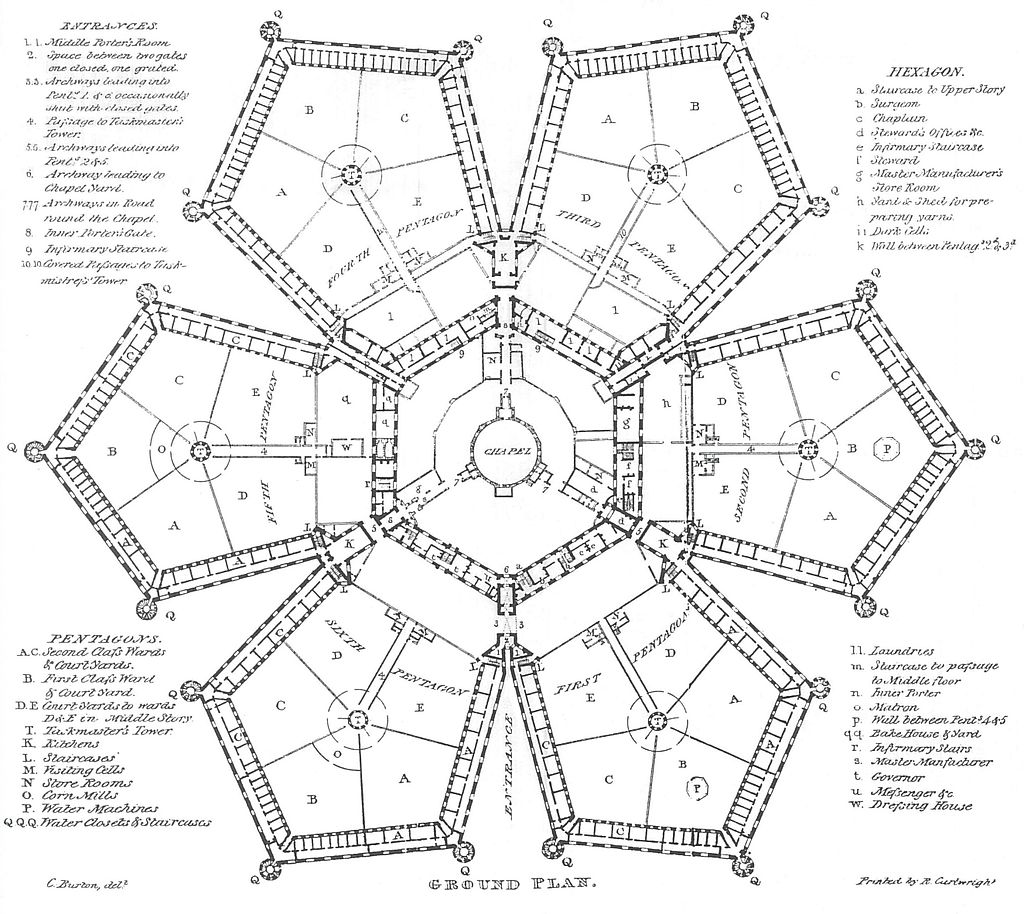
\includegraphics[width=0.8\textwidth]{MillbankPlan}}
    \caption{نقشه زندان میلیبنک مبتنی بر طراحی پنوپتیکون
      %\citep{kim2016integrated}
    }
    \label{fig:MillbankPlan}
  \end{figure}\\

\fi %Dataveillance
% * from old proposal and thesis fron khordad 1400 /media/d_drive/PJ/K/C/PJ-HDD-NiliLab/ssd2-laptop-backup-4mordad00/PJ/KN/Cog/proposal/tex/003
به نظر می‌رسد تصمیم‌گیرندگانی که در چنین سازمان‌هایی حضور دارند به حجم زیادی از اطلاعات
شخصی افراد دسترسی دارند. اگر این اطلاعات که در ابتدا با رضایت افراد و فقط جهت بهینه سازی ارائه خدمات مورد توافق جمع‌آوری شده‌است، با نهادهای ثانویه
به اشتراک گذاشته شود، می‌تواند برای نظارت و تغییر رفتار هدفمند استفاده شود. به این ترتیب
\textit{
  \gls{Social networking service}
}
به طور غیر مستقیم و بالقوه سبب ساز تغییرات اجتماعی خارج از کنترل و آگاهی کاربران شبکه های اجتماعی، که فراهم کنندگان و صاحبان اصلی
اطلاعات هستند، می‌شوند.
افراد تصمیم‌گیرنده در این سازمان‌ها به علت وظیفه‌ای که در قبال سازمان
متبوع خود دارند، ملزم به حداکثر کردن سود بنگاه‌های اقتصادی‌ای هستند
که مالکیت این سازمان‌ها و سرویس‌های ارائه شده را، در اختیار
دارند. تصمیم در به اشتراک گذاری اطلاعات از سوی این افراد، معمولا در وهله اول می‌تواند بر اساس چنین انگیزه‌ای مطابق با قواعد نظام‌های سرمایه‌داری و منطقی به نظر برسد.
اما از طرف دیگر، همین تصمیمات می‌تواند باعث متضرر شدن
کاربرانی باشد که مالک اصلی اطلاعات جمع‌آوری شده می‌باشند. در چنین شرایطی، وقتی که
\textit{
  \glspl{Oversight institution}
}
با تغییرات سریع  در ساختارهای
\textit{
  \glspl{Information society}
}
ناهماهنگ هستند
\!\citep{cavoukianDiscussionPaperPrivacy2009,machovaDiscourseSurveillancePrivacy2021}،
بررسی ساز و کار موثر بر تصمیمات این افراد، اهمیت پیدا می‌کند.


اهمیت  این موضوع زمانی بیشتر می‌شود که کاربران
\textit{
  \gls{Social networking service}
}
تحت تاثیر
\textit{
  \glspl{Motivitions of}
}
متضاد قرار می‌گیرند و رفتاری را نشان می‌دهند که با عنوان
\textit{
  \gls{Privacy paradox}
}
شناخته می‌شود
\!\citep{barthPrivacyParadoxInvestigating2017}.
این تناقض به عدم تناسب میان رفتار کاربران شبکه‌های اجتماعی با آگاهی بالای آنها از پیامدهای این رفتارها، اشاره دارد.
این تناقض زمانی مشاهده می‌شود که کاربران شبکه‌های اجتماعی با وجود اهمیتی که برای حفظ
\textit{
  \gls{Information privacy}
}
قائل هستند،  باز هم بی‌محابا نسبت به  منتشر کردن اطلاعات شخصی خود
در شبکه‌های اجتماعی اقدام می‌کنند.

این رفتار حتی پس از روبرو شدن با
پیامدهای سوءاستفاده از این اطلاعات نیز کاهش چشمگیری نداشته است
\!\citep{hermesWhoQuitsPrivacyInvasive2021,wirthLazinessExplanationPrivacy2022}.
به نظر می‌رسد که جلوگیری از پیامدهای  نامطلوب سوءاستفاده از اطلاعات خصوصی کاربران و نقض
\textit{
  \gls{Information privacy}
}
از طریق مداخلاتی که در سطح رفتار کاربران انجام شود، با توجه به گسترش و تنوع جمعیتی،
دشوار خواهد بود. با این وجود،
\textit{
  \gls{Information privacy}
}
که به توانایی افراد
برای کنترل اطلاعات مربوط به آنها اشاره دارد
\!\citep{smithInformationPrivacyMeasuring1996}
در سال‌های اخیر بیشتر مورد توجه کاربرانی قرار گرفته است
که داده‌های آنها توسط
\textit{
  \glspl{Social networking service}
}
جمع‌آوری، طبقه‌بندی و تحلیل می شود
\!{\citep{wallOrganizationalViolationsExternally2016}.
\textit{
  \gls{Information privacy}
}
با اشتراک‌گذاری اطلاعات شخصی توسط صاحب اطلاعات، در تضاد نیست.
\textit{
  \gls{Information privacy}
}
داشتن کنترل بر روی اطلاعات بعد از به  اشتراک‌گذاری، می‌باشد.\citep{acquistiEconomicsPrivacy2016}}.
به اشتراک گذاری اطلاعات شخصی از دید صاحبان اولیه اطلاعات،
به عنوان یک رفتار اجتماعی ناخوشایند و بالقوه ناهنجار، شناسایی شده است
\citep{norbergCopingInformationRequests2014}،
اما به نظر می‌رسد چنین دیدگاهی با تعریفی که برای
\textit{
  \gls{Information privacy}
}
ارائه شد، در تضاد قرار می‌گیرد. اگر کاربران بتوانند بعد از
\textit{
  \gls{Disclosure}
}
اطلاعات خود، بر روی نحوه استفاده از آن کنترل داشته باشند،
\textit{
  \gls{Personal Information Sharing Behavior}
}
به تنهایی
اثرات مخربی در پی نخواهد داشت.  به علاوه
جمع‌آوری و پردازش اطلاعات می‌تواند نتایج سازنده‌ای، در سطح اجتماعی و فردی داشته باشد
\citep{rockenbachProvidingPersonalInformation2020}.
امروزه افرادی که در
\textit{
  \glspl{Information society}
}
فاقد
\textit{
  \glspl{information record}
}
کافی در
\textit{
  \gls{Big data}
}
باشند، از جهات مختلف مورد
\textit{
  \gls{Discrimination}
}
قرار می‌گیرند
\!\citep{favarettoBigDataDiscrimination2019,lermanBigDataIts2013}.
با این دیدگاه، به اشتراک گذاری اطلاعات شخصی توسط صاحب اطلاعات، نه تنها
ناسازگارانه نیست، بلکه به یک رفتار
\textit{
  \gls{Prosocial}
}
تبدیل می‌شود.

اطلاعات کاربران پس از
\textit{
  \gls{Disclosure}
}
در اختیار تصمیم‌گیرندگانی قرار می‌گیرد که در
\textit{
  \glspl{Social networking service}
}
مسئول جمع‌آوری، ذخیره‌سازی و پردازش اطلاعات هستند. به نظر می‌آید که حفظ
\textit{
  \gls{Information privacy}
}
و جلوگیری از اثرات مخرب اجتماعی و فردی سوءاستفاده از
اطلاعات شخصی انباشته شده، از طریق شناسایی عوامل موثر
بر تصمیم‌گیری این افراد و به اجرا در آوردن
مداخلات موثر در این سطح،نتایج بهتری در پی داشته باشد.

کاربران
\textit{
  \glspl{Social networking service}
}
پس از ارائه اطلاعات شخصی خود، خدماتی را از آن دریافت می‌کنند. همان‌طور که اشاره شد، این
تبادل میان کاربر و
\textit{
  \glspl{Social networking service}
}
مورد توافق طرفین است. شرایط حاکم بر این تبادل در توافق‌نامه‌ای
که در زمان عضویت به افراد ارائه می‌شود، مشخص شده است. به عنوان مثال
فرد در قبال اطلاعات شخصی خود از امکانات
\textit{
  \glspl{Social networking service}
}
برای برقراری ارتباط با دوستان خود استفاده می کند. او همچنین
با شروط دیگری که  برای عضویت لازم بوده است، موافقت کرده است. او
قبول کرده است که
\textit{
  \gls{Social networking service}
}
اطلاعات شخصی‌اش را در جهت ارائه تبلیغات هدفمند به کاربران، ذخیره کند
و مورد بازبینی و پردازش قرار دهد. اثرات مخرب این تبادل از زمانی شروع می شود که دریافت کننده اطلاعات، از
آن برای اهدافی به غیر از توافق اولیه استفاده کند و یا امکان این کار را برای یک شخص ثالث فراهم کند
\!{\citep{padyabExploringImpactsSecondary2018}}.

\textit{
  \gls{Secondary use of information}
}،
استفاده از اطلاعات شخصی برای اهدافی فراتر
از توافق اولیه، بعد از
\textit{
  \gls{Disclosure}
}
اطلاعات شخصی توسط خود فرد، است. این عمل توسط موسسه جمع‌آوری کننده اطلاعات
و افراد تصمیم‌گیرنده در آن انجام می‌گیرد
\!{\citep{culnanHowDidThey1993}}.
پیامد‌های زیانبار تصمیمات بنگاه‌های اقتصادی و فن‌آوری بزرگی
مانند
\textit{
  \glspl{Meta}
}
برای استفاده ثانویه از اطلاعات شخصی جمع‌آوری شده، در پژوهش‌های مختلف بررسی شده اند
\!{\citep{padyabExploringImpactsSecondary2018}}.
این تصمیمات در سال‌های ۲۰۱۵ تا ۲۰۱۸، منجر به ناهنجاری‌های وسیع در سطح جوامع شدند.
پیامدهای این ناهنجاری‌ها در نهایت افراد عضو جوامع را به طور غیر مستقیم
تحت تاثیر قرار می‌دهند. این افراد، متشکل از همان کاربرانی هستند که به طور جمعی، تامین کننده
داده‌های جمع‌آوری شده توسط
\textit{
  \glspl{Meta}
}
بوده‌اند.
\!{\citep{redmanDataCredibilityProblem2013,dezwartSurveillanceBigData2014,spiekermannNetworksControlReport2016,schyffDuplicitousSocialMedia2020}}.
با وجود آسیب‌پذیری افراد از داده‌های شخصی جمع‌آوری شده توسط شرکت‌ها
و شرکای تجاری آنها، تحقیقات نشان می‌دهد
که کاربران این جنبه تبادل اطلاعات خود را نادیده می‌گیرند
\!{\citep{raynes-goldieAliasesCreepingWall2010,brandtzaegTooManyFacebook2010,youngPrivacyProtectionStrategies2013}}،
هرچند با توجه به تاثیرات سازنده‌ای که برای رفتار اشتراک گذاری اطلاعات در بخش‌های
قبلی نام برده شده است، به نظر می‌رسد که می‌توان، عدم تغییر رفتار کاربران در به اشتراک گذاری اطلاعات خود را
\textit{
  \gls{post–Cambridge Analytica scandal era}
}
\!{\citep{epsteinViewFramingDigital2021}}
، پدیده مطلوبی توصیف کرد. با این وجود وقوع چنین پدیده‌هایی به
\textit{
  \gls{Trust}
}
در افراد جامعه آسیب می‌زند و در نهایت سبب کاهش منافع جمعیِ جمع‌آوری و پردازش اطلاعات، می‌گردد.


\gls{Cambridge Analytica scandal}
در سال ۲۰۱۶ باعث پی‌گیری‌ حقوقی شرکت
\glspl{Meta}
و مدیرعامل آن
\textit{
  \gls{Mark Zuckerberg}
}
و محکومیت به پرداخت جریمه پنج میلیارد دلاری، شد
.\!{\citep{daviesFacebookPay5bn2019,smoutFacebookAgreesPay2019}}
واکنش مسؤولین فیسبوک نشان می‌دهد
که افراد تصمیم گیرنده در شرکت‌های جمع‌آوری کننده
اطلاعات نیز احتمالا از پیامدهایی که سیاست‌گذاری‌های آنها در استفاده ثانویه از اطلاعات شخصی کاربران
برای خود شرکت در پی دارد، ناآگاه هستند
\!{\citep{grewalSuspendingCambridgeAnalytica2018,kozlowskaFacebookDataPrivacy2018}}
\!. با توجه به اینکه این افراد مسؤول حداکثر
کردن سود شرکت‌های خود هستند،
به نظر می‌رسد که چنین تصمیماتی فرض
\glspl{Rational}
بودن عامل‌های تصمیم‌گیرنده در
\glspl{Rational choice theory}
را به چالش می‌کشد. با در نظر گرفتن این مساله‌، ما در این پژوهش از از یک چارچوب نظری که فرض
\textit{
  \gls{Rational}
}
بودن تصمیمات را به چالش می‌کشد برای
\textit{
  \glspl{Articulation}
}
مفاهیم و رویکردهایمان استفاده کردیم.

\section*{نظریه رفتار برنامه‌ریزی‌شده و اهمیت استفاده ثانویه از اطلاعات}
تحقیقات زیادی برای بررسی رفتار کسانی که
اطلاعات خود را در اینترنت به اشتراک می‌گذارند انجام شده است
\!\!{\citep{kamleitnerInformationSharingPrivacy2019,kamleitnerYourDataMy2019}}.
همچنین رفتار افرادی که در مالکیت اطلاعت با فرد دیگر، شریک هستند بررسی شده است
\!\!{\citep{tawnieInterdependentPrivacy2017}}.
نتایج نشان می‌دهد که با وجود اینکه در همه جهان
\!،
\textit{
  \gls{Privacy}
}
اطلاعات شخصی افراد مساله مهمی برای کاربران آنلاین
است، بیشتر کاربران به ندرت برای محافظت از این داده، به خود زحمت می‌دهند و حتی در
بیشتر مواقع به طور داوطلبانه آن‌را پخش می‌کنند. تلاش زیادی انجام شده است تا این
دوگانگی میان
\textit{
  \gls{Privacy Attitude}
}
و رفتار، که معمولا با عنوان
\textit{
  \gls{Privacy paradox}
}
شناخته می‌شود، توضیح داده شود
\!{\citep{gerberExplainingPrivacyParadox2018}}.
به طور مشابه پژوهشی که در زمینه رفتار
\textit{
  \gls{Trust}
}
با به کار بردن
\textit{
  \gls{Theory of planned behavior}
}
در
\textit{
  \gls{Trust game}
}
انجام شده است،  وجود چنین تناقضی را در افراد
\textit{
  \gls{Trustor}
}
نیز نشان می‌دهد
\!\citep{gazdagNotWantTrust2019}.
به طور کلی، تا کنون  تحقیقات زیادی در حوزه
\textit{
  \gls{Information privacy}
}،
از
\textit{
  \gls{Trust game}
}
برای بررسی رفتار افراد در این تعامل
\textit{
  \gls{Interpersonal}
}،
استفاده کرده اند. با وجود اینکه تا به امروز رفتار کاربرانی که اطلاعات
\!(یا اطلاعات مشترک)
خود را به اشتراک می‌گذارند، مورد کنکاش قرار گرفته است، حیطه
رفتاری افرادی که دریافت کننده این  اطلاعات هستند به ندرت
مورد توجه قرار گرفته است
\!\citep{demmersYourDataAre2021}.

% \subsection{کمبریج آنالیتیکا و استفاده ثانویه از اطلاعات}
\section{کمبریج آنالیتیکا و استفاده ثانویه از اطلاعات}
در سال ۲۰۱۳ استاد دانشگاه کمبریج یک برنامه به نام
«\lr{thisisyourdigitallife}»
ساخت. این برنامه در شبکه اجتماعی فیسبوک به کاربران
آزمون‌های شخصیت‌شناسی ارائه می‌کرد. وقتی کاربر فیسبوک برنامه را بر روی حساب کاربری خود فعال و نصب
می‌کرد، برنامه جمع‌آوری اطلاعات شخصی او را آغاز می‌کرد. این اطلاعات شامل اطلاعات حساب کاربری و فعالیت‌های کاربر در فیسبوک
بود. فعالیت‌هایی مانند اینکه کاربر کدام محتوای فیسبوک را لایک کرده است. در حدود سیصد هزار نفر این
برنامه را نصب کردند. اما اطلاعاتی که جمع‌آوری شد به این تعداد محدود نماند.
این برنامه اطلاعاتی درباره دوستان کاربر که تنظیمات حریم خصوصی خود را درست  تنظیم نکرده بودند، را
نیز جمع‌آوری کرد. در نتیجه برنامه توانست اطلاعات ۸۷ میلیون نفر را جمع‌آوری کند
\!\citep{kangFacebookSaysCambridge}.

سپس دکتر کوگان داده چمع‌آوری شده را به شرکت
\textit{
  \gls{ Strategic Communication Laboratories (SCL)}
}
که مالک شرکت کمبریج آنالیتیکا است، انتقال داد. این شرکت یک موسسه مشاوره
سیاسی بود که از داده برای شناسایی ویژگی‌های شخصیتی و رفتار رای دهندگان
استفاده می‌کرد
\!\citep{rosenbergHowTrumpConsultants2018}.
این شرکت از این داده برای کمک به به پویش محافظه‌کاران برای هدف
قرار دادن تبلیغات اینترنتی و پیام رسان‌ها استفاده کرد. این همان عملی
بود که دکتر کوان شرایط و مقررات فیبوک را نقض کرد که انتقال یا
فروش داده به هر شبکه تبلیغاتی ، دلال داده یا هر سرویس تبلیغاتی
و درآمد‌زایی، ممنوع می‌کرد
\!\citep{granvilleFacebookCambridgeAnalytica2018}.

وقتی در سال ۲۰۱۵ فیسبوک از این موضوع مطلع شد، برنامه دکتر کوگان
را حذف  کرد و از کوگان و کمبریج آنالیتیکا درخواست کرد که
مدرکی ارائه دهند، که داده را پاک کرده‌اند. کوگان و کمبریج آنالیتیکا
به فیسبوک تاییده‌ای ارائه دادند که داده را حذف کرده‌اند. هرچند  کپی داده
خارج از کنترل فیسبوک باقی ماند.  وقتی الکساندر نیکس، مدیر عامل
کمبریج آنالیتیکا، به قانون‌گذاران گفت که شرکتش داده‌های فیسبوک را در
اختیار ندارد، یکی از کارمندان گفت که او اخیرا صدها گیگابایت داده را
بر روی سرورهای کمبریج آنالیتیکا دیده‌است و اطلاعات رمز نگاری نشده بودند.

در سال ۲۰۱۵، فیسبوک هیچ بیانیه عمومی‌ای درباره این رخداد منتشر نکرد. همچنین
کاربرانی که اطلاعات‌شان با کمبریج آنالیتیکا به اشتراک گذاشته شده
بود. همچنین فیسبوک به کمیته تجارت فدرال، درباره این موضوع
چیزی نگفت. بر اساس آنچه که مارک زاکربرگ در کنفرانس دو روزه
استماع‌اش در نهم و دهم آوریل ۲۰۱۸ گفت، به محض اینکه گواهی کمبریج آنالیتیکا
مبنی بر حذف و تعهد عدم استفاده از داده را دریافت کردند، فیسبوک
موضوع را خاتمه یافته تلقی کرد
\!\citep{spanFacebookCEOMark}.

با منتشر شن این داستان در مارس ۲۰۱۸ در دو نشریه بین‌المللی، فیسبوک
مطلع شد که داده تا آن روز پاک نشده بوده است. نتایج به بار آمده
چنین حادثه‌ای بی سابقه بود. فیسبوک توسط چند نهاد قضایی در ایالت متحده،
جزیره انگلستان و اتحادیه اروپا مورد بازخواست قضایی قرار گرفت. یک پویش
فیسبوک را حذف کنید راه افتاد و افت شدید قیمت سهام باعث شد تقریبا پنجاه میلیارد دلار
سرمایه شرکت در عرض سه روز پس از فاش شدن اخبار، از بین رفت.




%   \glspl{phenomenon of dyadic completion}
%   نشان می دهد که گرایش های
%   \glspl{deontological}
%   و
%   \glspl{utilitarian}
%   نه تنها به طور همزمان فعال هستند
%   بلکه اغلب سازگار و تقویت کننده می‌باشند
%   \!{\citep{grayTwoMindsVs2012}}.
% \subsection{چارچوب‌های نظری}
% ^ %%%%%%%%%%%%%%%%%%%%%%%%%%%%%%%%%%%%%%%%%%%%%%%%%%%%%%%%%%%%%
% ^ %%%%%%%%%%%%%%%%%%%%%%%%%%%%%%%%%%%%%%%%%%%%%%%%%%%%%%%%%%%%%
% ^ %%%%%%%%%%%%%%%%%%%%%%%%%%%%%%%%%%%%%%%%%%%%%%%%%%%%%%%%%%%%%
\section{اهمیت}
%% توضیح بیشتر اضافه گردد بعدا
پژوهش انجام شده در سال ۲۰۲۰ نشان می دهد که در بازار داده های خصوصی آنلاین بازیگران زیادی به عنوان واسطه وجود دارند.
\!\citep{agogoInvisibleMarketOnline2021}
همچنین با گسترش هر روزه سیستم های اطلاعاتی که به
جمع‌آوری، ذخیره‌سازی، پردازش و به‌اشتراک‌گذاری داده‌های
خصوصی افراد می‌پردازند بررسی فرایندهای
تصمیم گیری و پارامتر‌های تاثیر گذار
بر این تصمیم‌گیری دارای اهمیت شده است
\!.
\!\citep{spiekermannValuesEthicsInformation2022}
از سوی دیگر نگرش افراد تصمیم گیرنده نسبت به ارزش اطلاعات خصوصی افراد می تواند نقش مهمی در رفتار آنها داشته باشد.
پژوهش‌هایی برای اندازه‌گیری ارزش داده‌های خصوصی انجام شده است
\!\citep{  fastValuePersonalData2021a,wesselsSellNotSell2019,tangHowChineseWeb2021}
\ifWillingnessToPay
  مقایسه میان رفتار افراد در پژوهش‌های اندازه‌گیری
  \textit{تمایل به پرداخت}
  \LTRfootnote{willingness to pay}
  نشان داده است که
  \textit{تمایل به پرداخت }
  با استفاده از روش‌های فرضی مانند
  \textit{ارزشيابی مشروط}
  \LTRfootnote{contingent valuation }
  میان ۱۷ تا ۶۳ درصد بالاتر
  از روشهای غیر فرضی مانند
  \textit{حراج تجربی}
  \LTRfootnote{experimental auction}
  است.
  حراج تجربی به عنوان یک روش
  \textit{سازگار با انگیزه}
  \LTRfootnote{incentive compatibility}
  شناسایی شده‌است
  \!\citep{martinez-carrascoComparingHypotheticalNonhypothetical2015}
  .
  یک فرایند،
  \textit{سازگار با انگیزه}
  است وقتی‌که همه شرکت‌کنندگان فقط  با درنظر گرفتن ترجیهات واقعی خود، بهترین خروجی را بدست می‌آورند
  \!\citep{nisanAlgorithmicGameTheory2007}
  \!.

  % ^ %%%%%%%%%%%%%%%%%%%%%%%%%%%%%%%%%%%%%%%%%%%%%%%%%%%%%%%%%%%%%
  % ^ %%%%%%%%%%%%%%%%%%%%%%%%%%%%%%%%%%%%%%%%%%%%%%%%%%%%%%%%%%%%%
  % ^ %%%%%%%%%%%%%%%%%%%%%%%%%%%%%%%%%%%%%%%%%%%%%%%%%%%%%%%%%%%%%
\fi
\section{نظریه‌ها}
\textit{
  \gls{Rational choice theory}
}
\!{\citep{beckerEconomicApproachHuman1978}}،
این فرض را بنا می‌نهد که انسان‌ها بر اساس
تابعی از مجموع منفعت، با کسر مجموع هزینه‌های یک تصمیم
یا مبادله و برای حداکثر کردن فایده  شخصی دست به عمل می‌زنند.

این موضوع پایه‌ای برای طرح نظریه
\textit{
  \gls{Theory of reasoned action}
}
توسط
\textit{
  \gls{Icek Ajzen}
}
و
\textit{
  \gls{Martin Fishbein}
}
در در دهه ۸۰ میلادی شد. این نظریات پیشنهاد می‌کنند که بین
\textit{
  \gls{Atteutude}
}
و رفتار رابطه وجود دارد
\!{\citep{ajzenPredictionGoaldirectedBehavior1986}}.
فهم رفتار اختیاری افراد به وسیله
بررسی انگیزه‌هایی که باعث اجرای یک عمل می شود، هدف اصلی این نظریه بود. این نظریه
بیان می کند که قصد اجرای یک عمل پیش‌بینی‌کننده اصلی انجام یا عدم ایجاد رفتار  است. به
علاوه پارامتر هنجاری
(هنجارهای اجتماعی که عمل را احاطه کرده‌اند)
در اجرا شدن یا نشدن عمل نقش بازی می کند
\!{\citep{HealthBehaviorTheory2015,doswellTestingTheoryReasoned2011,ajzenAttitudesAttitudeBehaviorRelation2000}}
.
اما تحقیقاتی که در قالب چارچوب‌های
\textit{
  \gls{Behavioral economics}
}
انجام شد، این فرض را مورد تردید قرار داده اند
\!\citep{henrichEconomicManCrosscultural2005}.
برای رفع کاستی‌های
\textit{
  \gls{Theory of reasoned action}
}
آیزن در سال ۱۹۹۱
\!\citep{ajzenTheoryPlannedBehavior1991}
\textit{
  \gls{Theory of planned behavior}
}
را مطرح کرد. به بیان این تئوری سه پارامتر اصلی
\textit{
  \gls{Attitude}
}
\!،
\textit{\gls{Subjective norm}}
و
\textit{\gls{Perceived Behavioral control}}
\!،
\textit{\glspl{Behavioral intention}}
افراد را شکل می‌بخشند. پایه تفکر
\textit{
  \gls{Theory of planned behavior}
}
این است که
\textit{
  \gls{Personal Information Sharing Behavior}
}
از تعامل
\textit{\glspl{Psychological construct}}
\textit{
  \gls{Attitude}
}
\!،
\textit{\gls{Subjective norm}}،
\textit{\gls{Perceived Behavioral control}}
و
\textit{\glspl{Behavioral intention}}
نسبت به
\textit{
  \gls{Personal Information Sharing}
}،
ایجاد می‌شود.

در پژوهش‌های پیشین برای بررسی
\textit{
  \gls{Personal Information Sharing Behavior}
}
از
\textit{
  \gls{Theory of reasoned action}
}
\!\citep{malhotraInternetUsersInformation2004}،
و
\textit{
  \gls{Theory of planned behavior}
}
برای ایجاد ساختاری که روابط بین پارامترها را مدل می‌کند، استفاده شده است
\!\citep{dinevExtendedPrivacyCalculus2006b}.

در این پژوهش ما بررسی رفتار به اشتراک گذاری اطلاعات خصوصی دیگران در
\textit{
  \gls{Conceptual framework}
}
\textit{
  \gls{Theory of planned behavior}
}
پرداختیم.

برای سنجش رویکرد‍ افراد به
\textit{
  \gls{Personal information of Others}
}
یک پرسشنامه بر اساس دسته‌بندی‌های هفت‌گانه‌ای که در پژوهش پیشین با توجه به رویکرد صاحبان
اولیه اطلاعات خصوصی نسبت به خطر فاش شدن اطلاعات شخصی شان در حوزه‌های مختلف، ساخته شد.
این پرسشنامه برای هر دسته از سوالات دارای ۲ سوال است. برای اینکه بتوان باور
آزمودنی‌ها، را هم بر اساس ارزش ذهنی خود
\!(نگرش به ارزش اطلاعات)
و هم بر اساس ارزش ذهنی دیگران
\!(هنجار ذهنی و باور هنجاری)
و همچنین برای اندازه‌گیری پایایی درونی،
سوالات به دو دسته تقسیم ‌می‌شود.
به هر آزمودنی، دسته اول اطلاعات خصوصی به همراه یک سوال برای سنجش باور هنجاری، و دسته دوم
اطلاعات به همراه سوال دیگر برای سنجش باور شخصی، ارائه شد. به طور تصادفی این دو دسته از
سوالات برای هر آزمودنی جابجا شدند تا در نهایت پاسخ‌های نیمی از آزمونی‌ها به دسته اول سوالات از دید خود و نیمی
دیگر از آزمودنی ها به دسته دوم سوالات از دید خود، جمع‌آوری شوند. به همین ترتیب پاسخ به سوالات دسته اول و دوم
با توجه به باور هنجاری از دو دسته مستقل به تصادف انتخاب شدند، جمع‌آوری شد. تصادفی سازی در زمان وردو آزمودنی‌ها
به آزمایش با انتصاب افراد با احتمال ۵۰ درصد به دو گروه، انجام شد.
% * %%%%%%%%%%%%%%%%%%%%%%%%%%%%%%%%%%%%%%%%%% from old proposal and thesis from khordad 1400

\section{متغیر‌ها و پرسشنامه‌ها}

\ifPlennedBahaviorTheory
  \textit{\gls{Theory of planned behavior}}
  \!(TPB)
  % \LTRfootnote{Theory of planned behavior (TPB) }
  %  acronyms اضافه شود
  ، تعامل سه باور فردی شامل
  \textit{\gls{Atteutude}} ،
  \textit{\gls{Subjective norm}} و
  \textit{\gls{Perceived Behavioral control}}
  % \LTRfootnote{Perceived Behavioral control}
  را عامل رفتار می داند
  \!(شکل: \ref{fig:Theory_of_planned_behavior_chart})
  \!\citep{ajzenTheoryPlannedBehavior2020}.
  در این نظریه
  \textit{\gls{Atteutude}}
  از دو نگرش احساسی و نگرش ابزاری تشکیل شده است.
  \textit{\gls{Subjective norm}}
  شامل  هنجارهای ذهنی و هنجار توصیفی است.
  \textit{\gls{Perceived Behavioral control}}،
  دو بخش کنترل رفتاری درک شده و خود کارآمدی درک شده را شامل می باشد
  در این نظریه عامل اصلی تعیین کننده
  رفتار، قصد رفتاری است و اجزای ساختاری این نظریه
  بر روی قصد تاثیر ویژه‌ای دارند
  \citep{mhmdpwrBrrsyTthyrTywry2022}
  \begin{figure}[ht]
    \centerline{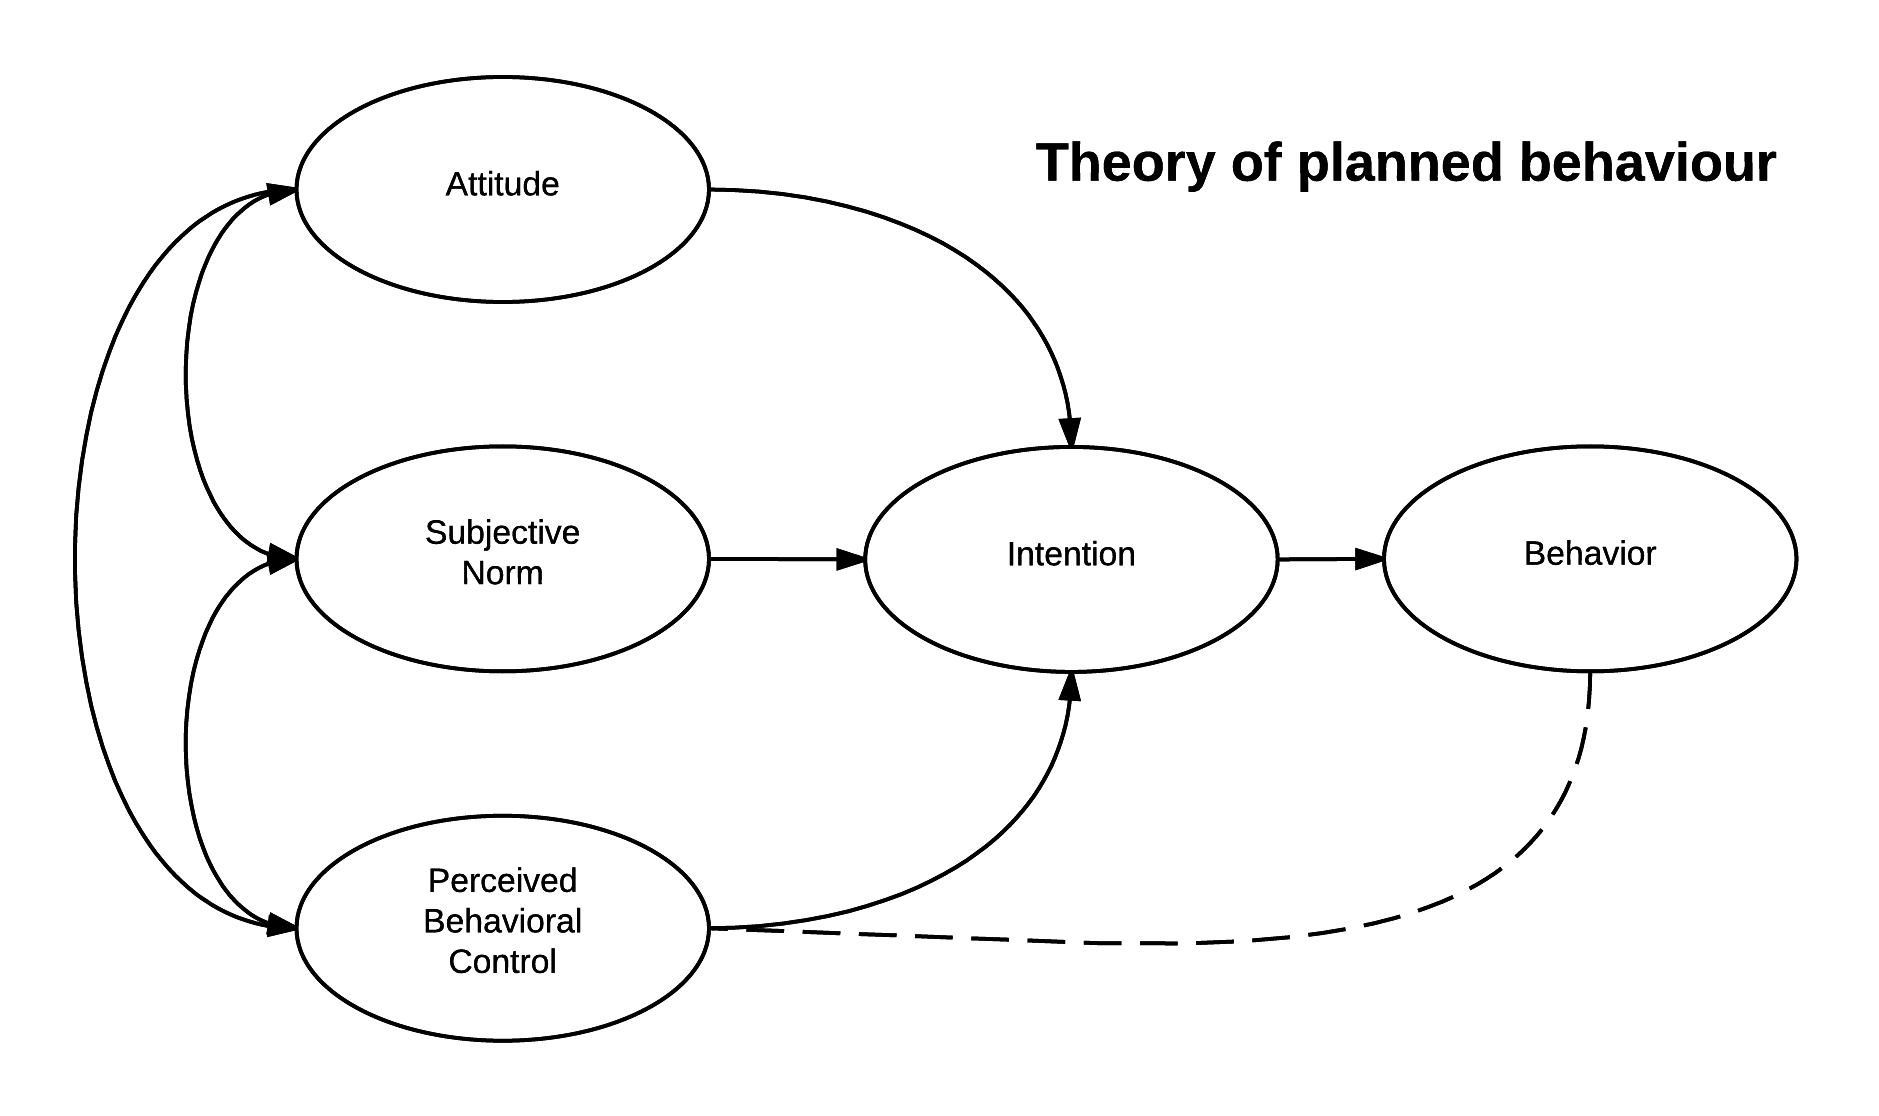
\includegraphics[width=0.8\textwidth]{Theory_of_planned_behavior_chart}}
    \caption{ساختار نظریه رفتار برنامه ریزی شده
      %\citep{kim2016integrated}
    }
    \label{fig:Theory_of_planned_behavior_chart}
  \end{figure}\\

  این نظریه در پژوهش‌های پیشین برای بررسی رفتار
  به اشتراک گذاری داده های خصوصی
  فرد در شبکه اجتماعی فیسبوک استفاده شده است
  \!\citep{vanderschyffInformationPrivacyBehavior2020}
  \!.
  مدلی که
  \!\gls{Theory of planned behavior}
  ارائه پیشنهاد می‌دهد، احتمال وقوع  رفتار‌های ارادی مخصوصا رفتار‌های ارادی مثبت به شدت تمایل فرد به
  انجام آن رفتار بستگی دارد.
  \!({\gls{Icek Ajzen}})
  عامل تعیین کننده برای انجام یک کار تمایلات او است.
\fi
%%%%%%%%%%%%%%%%%%%%

% \ifSurveyfillingBehavior
%   % بررسی اینکه آیا از نحوه پر کردن فرم ها می توان به کانفیدنس صداقت آزمودنی پی برد یا نه
%   در صورتیکه گزینه‌های پرسشنامه اجباری باشند کیفیت داده‌های جمع‌آوری شده کاهش می یابد.
%   \!\citep{sischkaImpactForcedAnswering2022}
% \fi

% ^ %%%%%%%%%%%%%%%%%%%%%%%%%%%%%%%%%%%%%%%%%%%%%%%%%%%%%%%%%%%%%
% ^ %%%%%%%%%%%%%%%%%%%%%%%%%%%%%%%%%%%%%%%%%%%%%%%%%%%%%%%%%%%%%
% ^ %%%%%%%%%%%%%%%%%%%%%%%%%%%%%%%%%%%%%%%%%%%%%%%%%%%%%%%%%%%%%

\section{فرضیه پژوهشی}

% ^ %%%%%%%%%%%%%%%%%%%%%%%%%%%%%%%%%%%%%%%%%%%%%%%%%%%%%%%%%%%%%
% ^ %%%%%%%%%%%%%%%%%%%%%%%%%%%%%%%%%%%%%%%%%%%%%%%%%%%%%%%%%%%%%
% ^ %%%%%%%%%%%%%%%%%%%%%%%%%%%%%%%%%%%%%%%%%%%%%%%%%%%%%%%%%%%%%

% کلیه فایل‌های لازم برای حروف‌چینی با کلاس فوق، داخل پوشه‌ای به نام
% \lr{tehran-thesis}
% قرار داده شده است. توجه داشته باشید که برای استفاده از این کلاس باید فونت‌های
% \lr{IRLotusICEE}
% و
% \lr{IRTitr}
% را داشته باشید (که همراه با این کلاس هست و نیاز به نصب نیست).
% قلم‌های
% \lr{IRLotusICEE}
% مستخرج از قلم‌های استاندارد
% \lr{IRLotus}
% شورای عالی اطلاع‌رسانی%
% \footnote{
% قلم‌های استاندارد
% \lr{IRFonts}
% از شورای عالی اطلاع‌رسانی، منطبق بر آخرین نسخه استاندارد یونیکد، استاندارد ملی ۶۲۱۹ و استاندارد
% \lr{Adobe Glyph Naming}
% هستند.
% }
% هستند که توسط دکتر بابایی‌زاده اصلاحاتی روی آنها صورت پذیرفته است: تبدیل صفر توپر به صفر توخالی (جهت تمایز بیشتر با نقطه) و اضافه شدن
% \textit{\textbf{حالت توپر و ایرانیک توأم}}،
% که این موارد در قلم‌های شورای عالی اطلاع‌رسانی وجود ندارد.

% \subsection{این همه فایل؟!}
% \label{muchFiles}
% از آنجایی که یک پایان‌نامه یا رساله، یک نوشته بلند محسوب می‌شود، لذا اگر همه تنظیمات و مطالب پایان‌نامه را داخل یک فایل قرار بدهیم، باعث شلوغی و سردرگمی می‌شود. به همین خاطر، قسمت‌های مختلف پایان‌نامه یا رساله  داخل فایل‌های جداگانه قرار گرفته است. مثلاً تنظیمات پایه‌ای کلاس داخل فایل
% \lr{tehran-thesis.cls}، 
% قسمت مشخصات فارسی پایان‌نامه داخل 
% \lr{faTitle.tex}،
% مطالب فصل اول داخل 
% \lr{chapter1.tex}
% و تنظیمات قابل تغییر توسط کاربر داخل 
% \lr{commands.tex}،
% قرار داده شده است.
% \textbf{
% 	فایل اصلی این مجموعه، فایل
% 	\lr{main.tex}
% 	می‌باشد.
% }
% % یعنی بعد از تغییر فایل‌های دیگر، برای دیدن نتیجه تغییرات، باید این فایل را اجرا کرد. بقیه فایل‌ها به این فایل، کمک می‌کنند تا بتوانیم خروجی کار را ببینیم.
% اگر به فایل 
% \lr{main.tex}
% دقت کنید، متوجه می‌شوید که قسمت‌های مختلف پایان‌نامه، توسط دستورهایی مانند 
% \lr{input}
% و
% \lr{include}
% به فایل اصلی، یعنی 
% \lr{main.tex}
% معرفی شده‌اند.
% با توجه به ساختار محتوایی دستورالعمل، در فایل
% \lr{main.tex}
% فرض شده که پایان‌نامه یا رساله شما، از ۵ فصل و تعدادی پیوست تشکیل شده است. با اینحال، شما می‌توانید به راحتی فصل‌ها و پیوست‌ها را با صلاحدید اساتید راهنما، کم و زیاد کنید. این کار، بسیار ساده است. فرض کنید بخواهید یک فصل دیگر هم به پایان‌نامه اضافه کنید. برای این کار، کافی است یک فایل با نام دلخواه مثلاً 
% \lr{chapter6}
% و با پسوند 
% \lr{.tex}
% بسازید و آن را داخل پوشه 
% \lr{tehran-thesis}
% قرار دهید و سپس این فایل را با دستور 
% \verb!\include{chapter6}!
% داخل فایل
% \lr{main.tex}
%  فراخوانی کنید.

% \subsection{از کجا شروع کنم؟}
% قبل از هر چیز، باید یک توزیع تِک مناسب مانند تک‌لایو
% \lr{(TeXLive)}
% را روی سیستم خود نصب کنید. تک‌لایو  را می‌توانید از 
%  \href{http://www.tug.org/texlive}{سایت رسمی آن}%
% \LTRfootnote{\lr{\url{http://www.tug.org/texlive}}}
%  دانلود کنید یا مستقیماً از مخازن توزیع لینوکس خود بگیرید (مثلاً در اوبونتو با دستور
% \LRE{\verb!sudo apt install texlive-full!}).
% برای نصب تک‌لایو و اجرای اسناد زی‌پرشین می‌توانید از
% \href{http://parsilatex.com/site/shop/}{دی‌وی‌دی مجموعه پارسی‌لاتک}%
% \LTRfootnote{\lr{\url{http://parsilatex.com/site/shop/}}}
% و فایل راهنمای موجود در آن هم کمک بگیرید.

% برای تایپ و پردازش اسناد لاتک باید از یک ویرایشگر مناسب استفاده کنید. ویرایشگرهای
% \lr{TeXWroks},
% \lr{TeXstudio},
% \lr{Texmaker}
% و
% \lr{BiDiTeXmaker}
% بدین منظور تولید شده‌اند. می‌توان ویرایش‌گر 
%  \href{https://bitbucket.org/srazi/biditexmaker3}{\lr{BiDiTeXmaker}}%
%  \LTRfootnote{\lr{\url{https://bitbucket.org/srazi/biditexmaker3}}}
% را که بویژه برای کار با زی‌پرشین و مطالب دوجهته بهبود یافته است، بهینه‌ترین ویرایشگر لاتک برای کار با اسناد فارسی عنوان کرد.

% حال اگر نوشتن \پ اولین تجربه شما از کار با لاتک است، توصیه می‌شود که یک‌بار به صورت اجمالی، کتاب «%
% \href{http://www.tug.ctan.org/tex-archive/info/lshort/persian/lshort.pdf}{مقدمه‌ای نه چندان کوتاه بر
% \lr{\LaTeXe}}%
% \LTRfootnote{\lr{\url{http://www.tug.ctan.org/tex-archive/info/lshort/persian/lshort.pdf}\hfill}}»
% ترجمه دکتر مهدی امیدعلی را مطالعه کنید. این کتاب، کتاب بسیار کاملی است که خیلی از نیازهای شما در ارتباط با حروف‌چینی را برطرف می‌کند.
% اگر تک لایو کامل را داشته باشید، این کتاب را هم دارید. کافیست در خط فرمان دستور زیر را بزنید:
% \begin{latin}
% 	\texttt{texdoc lshort-persian}
% \end{latin}
% اگر عجله دارید، برخی دستورات پایه‌ای مورد نیاز در پیوست \ref{app:latexIntro} بیان شده‌اند.

% بعد از موارد گفته شده، فایل 
% \lr{main.tex}
% و
% \lr{faTitle.tex}
% را باز کنید و مشخصات پایان‌نامه خود مثل نام، نام خانوادگی، عنوان پایان‌نامه و ... را جایگزین مشخصات موجود در فایل
% \lr{faTitle.tex}
%  کنید. نیازی نیست نگران چینش این مشخصات در فایل پی‌دی‌اف خروجی باشید، زیرا کلاس 
% \lr{tehran-thesis}
% همه این کارها را بطور خودکار برای شما انجام می‌دهد. در ضمن، موقع تغییر دادن دستورهای داخل فایل
% \lr{faTitle.tex}
%  کاملاً دقت کنید؛ این دستورها، خیلی حساس هستند و ممکن است با یک تغییر کوچک، موقع اجرا، خطا بگیرید. برای دیدن خروجی کار، فایل 
% \lr{faTitle.tex}
%  را 
% \lr{Save}
% (نه 
% \lr{Save As})
% کنید و بعد به فایل 
% \lr{main.tex}
% برگشته و آن را اجرا کنید%
% \footnote{
% 	البته فایلهای این مجموعه به گونه‌ای هستند که در
% 	\lr{TeXWorks} یا
% 	\lr{TeXstudio}
% 	بدون بازگشت به فایل اصلی، می‌توانید سند خود را اجرا کنید.
% }.
%  حال اگر می‌خواهید مشخصات انگلیسی \پ را هم عوض کنید، فایل 
% \lr{enTitle.tex}
% را باز کنید و مشخصات داخلش را تغییر دهید.
% %\RTLfootnote{
% %برای نوشتن پروژه کارشناسی، نیازی به وارد کردن مشخصات انگلیسی پروژه نیست. بنابراین، این مشخصات بطور خودکار، نادیده گرفته می‌شود.
% %}
% در اینجا هم برای دیدن خروجی باید این فایل را ذخیره کرده، بعد به فایل 
% \lr{main.tex}
% برگشته و آن را اجرا کرد.

% برای راحتی بیشتر، کلاس 
% \lr{tehran-thesis.cls}
% طوری طراحی شده است که کافی است فقط  یک‌بار مشخصات \پ را (در فایل‌های
% \lr{faTitle.tex}
% و
% \lr{enTitle.tex})
% وارد کنید و هر جای دیگر که این مشخصات لازم باشند، به طور خودکار درج می‌شوند. با این حال، اگر مایل بودید، می‌توانید تنظیمات موجود را تغییر دهید؛ گرچه، در صورتیکه کاربر مبتدی هستید و یا با ساختار فایل‌های  
% \lr{cls}
%  آشنایی ندارید، بهتر است به فایل 
% \lr{tehran-thesis.cls}
% دست نزنید.

% نکته دیگری که باید به آن توجه کنید این است که در قالب آماده شده، سه گزینه به نام‌های
% \lr{bsc}،
% \lr{msc}
% و
% \lr{phd}
% برای نوشتن پروژه، پایان‌نامه و رساله، در نظر گرفته شده است. بنابراین اگر قصد تایپ پروژهٔ کارشناسی، پایان‌نامهٔ کارشناسی ارشد یا رسالهٔ دکتری را دارید، به ترتیب باید از گزینه‌های
% \lr{bsc}،
% \lr{msc}
% و
% \lr{phd}
% در فایل 
% \lr{main.tex}
% استفاده کنید. با انتخاب هر کدام از این گزینه‌ها، تنظیمات مربوط به آنها به طور خودکار، اعمال می‌شود.


% \subsection[مطالب پایان‌نامه را چطور بنویسم؟]
% {مطالب \پ را چطور بنویسم؟}
% \subsubsection{نوشتن فصل‌ها}
% همان‌طور که در بخش \ref{muchFiles} گفته شد برای جلوگیری از شلوغی، قسمت‌های مختلف \پ از جمله فصل‌ها، در فایل‌های جداگانه‌ای قرار داده شده‌اند. 
% مثلاً اگر می‌خواهید مطالب فصل ۱ را تایپ کنید، باید فایل‌های 
% \lr{main.tex}
% و
% \lr{chapter1.tex}
% را باز کرده و مطالب خود را جایگزین محتویات داخل 
% \lr{chapter1.tex}
% نمایید. دقت شود که در ابتدای برخی فایلها دستوراتی نوشته شده است و از شما خواسته شده که آن دستورات را حذف نکنید.

%توجه کنید که همان‌طور که قبلاً هم گفته شد، تنها فایل قابل اجرا، 
%\lr{main.tex}
%است. لذا برای دیدن حاصل (خروجی) فایل خود، باید  
%\lr{chapter1.tex}
%را ذخیره کرده و سپس فایل 
%\lr{main.tex}
%را اجرا کنید.

% نکته بسیار مهمی که در اینجا باید گفته شود این است که سیستم \lr{\TeX}، محتویات یک فایل تِک را به ترتیب پردازش می‌کند.  بنابراین، اگر مثلاً  دو فصل اول خود را نوشته و خروجی آنها را دیده‌اید و مشغول تایپ مطالب فصل ۳ هستید، بهتر است
% که دو دستور 
% \verb!% !TeX root=main.tex
% دستور زیر باعث شماره‌بندی صفحات فصول از ۱ می‌شود و باید در اولین فصل شما باشد. آن را حذف نکنید!
\pagenumbering{arabic} % 1, 2, ...

\chapter{مقدمه}
% دستور زیر باعث عدم‌نمایش شماره صفحه در اولین صفحه‌ی این فصل می‌شود.
%\thispagestyle{empty}
\ifDataveillance
  \textit{کریستین فوکس}
  \LTRfootnote{Christian Fuchs}
  جامعه شناس اتریشی،
  \textit{
    \gls{Social networking service}
  }
  \!({\lr{SNS}})
  در دنیای مدرن را به یک
  \textit{
    \gls{Panopticon}
  }
  تشبیه می کند   که در آن شرکت‌های بزرگی مانند
  \textit{
    \gls{Alphabet}
  }
  \!(
  شرکت مادر سرویس
  \textit{
    \gls{Google}
  }
  \!)
  و
  \textit{
    \gls{Meta}
  }
  \!(
  \!شرکت مادر و مالک برنامه‌های نرم‌افزاری مانند
  \textit{
    \gls{Instagram}
  }،
  \textit{
    \gls{Facebook}
  }
  و
  \textit{
    \gls{Whatsapp}
  }
  \!)
  به
  \textit{
    \gls{Dataveillance}
  }
  اعضا می‌پردازند
  \!\citep{romelePanopticismNotEnough2017a}.
  عبارت
  \textit{
    \gls{Panopticon}
  }
  را اولین بار
  \textit{
    \gls{Jeremy Bentham}
  }
  \!
  \citep{benthamPanopticonInspectionHouseContaining1791}
  برای توصیف ساختار‌های اجتماعی که مانند سیستم متمرکز نظارت عمل می‌کنند، از معماری وارد
  \textit{
    \gls{Social philosophy}
  }
  کرد.
\fi %Dataveillance
% * from old proposal and thesis fron khordad 1400 /media/d_drive/PJ/K/C/PJ-HDD-NiliLab/ssd2-laptop-backup-4mordad00/PJ/KN/Cog/proposal/tex/003
به نظر می‌رسد تصمیم‌گیرندگانی که در چنین سازمان‌هایی حضور دارند به حجم زیادی از اطلاعات
شخصی افراد دسترسی دارند. چنین افرادی، به علت وظیفه‌ای که در قبال سازمان
متبوع خود دارند، ملزم با حداکثر کردن سود بنگاه‌های اقتصادی هستند
که مالکیت این سازمان‌ها و سرویس‌های ارائه شده را، در اختیار
دارند.از طرف دیگر، همین تصمیمات می‌تواند باعث متضرر شدن
کاربرانی باشد که مالک اصلی اطلاعات جمع‌آوری شده می‌باشند. در چنین شرایطی، وقتی که
\textit{
  \glspl{Oversight institution}
}
با تغییرات سریع  در ساختارهای
\textit{
  \glspl{Information society}
}
ناهماهنگ هستند
\!\citep{cavoukianDiscussionPaperPrivacy2009,machovaDiscourseSurveillancePrivacy2021}،
بررسی ساز و کار موثر بر تصمیمات این افراد، اهمیت پیدا می‌کند.
اهمیت  این موضوع زمانی بیشتر می‌شود که کاربران
\textit{
  \gls{Social networking service}
}
تحت تاثیر
\textit{
  \glspl{Motivitions of}
}
متضاد قرار می‌گیرند و رفتاری را نشان می‌دهند که با عنوان
\textit{
  \gls{Privacy paradox}
}
شناخته می‌شود
\!citep{barthPrivacyParadoxInvestigating2017}.

این رفتار زمانی مشاهده می‌شود که کاربران شبکه‌های اجتماعی با وجود اهمیتی که برای حفظ
\textit{
  \gls{Information privacy}
}
بیان می‌کنند باز هم بی‌محابا نسبت به  منتشر کردن اطلاعات شخصی خود
در شبکه‌های اجتماعی اقدام می‌کنند.

این رفتار حتی پس از آگاه شدن از
پیامدهای سوءاستفاده از این اطلاعات نیز کاهش چشمگیری نداشته است
\!\citep{hermesWhoQuitsPrivacyInvasive2021,wirthLazinessExplanationPrivacy2022}.
به نظر می‌رسد که جلوگیری از پیامدهای  نامطلوب سوءاستفاده از اطلاعات خصوصی کاربران و نقض
\textit{
  \gls{Information privacy}
}
از طریق مداخلاتی که در سطح کاربران انجام شود، با توجه به گسترش و تنوع جمعیتی،
دشوار خواهد بود. با این وجود،
\textit{
  \gls{Information privacy}
}
که به توانایی افراد
برای کنترل اطلاعات مربوط به آنها اشاره دارد
\!{\cite{smithInformationPrivacyMeasuring1996}}
در سال‌های اخیر بیشتر مورد توجه کاربرانی قرار گرفته است
که داده‌های آنها توسط
\textit{
  \glspl{Social networking service}
}
جمع‌آوری، طبقه‌بندی و تحلیل می شود
\!{\cite{wallOrganizationalViolationsExternally2016}}
\!.
\textit{
  \gls{Information privacy}
}
با اشتراک‌گذاری اطلاعات شخصی توسط صاحب اطلاعات، در تضاد نیست.
\textit{
  \gls{Information privacy}
}
داشتن کنترل بر روی اطلاعات بعد از به  اشتراک‌گذاری، می‌باشد.
\!{\cite{acquistiEconomicsPrivacy2016}}.
به اشتراک گذاری اطلاعات شخصی از دید صاحبان اولیه اطلاعات،
به عنوان یک رفتار اجتماعی ناخوشایند و بالقوه ناهنجار، شناسایی شده است،
\!{\cite{norbergCopingInformationRequests2014}}،
اما به نظر می‌رسد چنین دیدگاهی با تعریفی که برای
\textit{
  \gls{Information privacy}
}
ارائه شد، در تضاد قرار می‌گیرد. اگر کاربران بتوانند بعد از
\textit{
  \gls{Disclosure}
}
اطلاعات خود، بر روی نحوه استفاده از آن کنترل داشته باشند،
\textit{
  \gls{Personal Information Sharing Behavior}
}
به تنهایی
اثرات مخربی در پی نخواهد داشت.  به علاوه
جمع‌آوری و پردازش اطلاعات می‌تواند نتایج سازنده‌ای، در سطح
اجتماعی و فردی داشته باشد
\!\citep{rockenbachProvidingPersonalInformation2020}.
افرادی که در
\textit{
  \glspl{Information society}
}
فاقد
\textit{
  \glspl{information record}
}
کافی در
\textit{
  \gls{Big data}
}
باشند، از جهات مختلف مورد
\textit{
  \gls{Discrimination}
}
قرار می‌گیرند
\!\citep{favarettoBigDataDiscrimination2019,lermanBigDataIts2013}.
با این دیدگاه، به اشتراک گذاری اطلاعات شخصی توسط صاحب اطلاعات، نه تنها
ناسازگارانه نیست، بلکه به یک رفتار
\textit{
  \gls{Prosocial}
}
تبدیل می‌شود. اطلاعات کاربران پس از
\textit{
  \gls{Disclosure}
}
در اختیار تصمیم‌گیرندگانی قرار می‌گیرد که در
\textit{
  \glspl{Social networking service}
}
مسئول جمع‌آوری، ذخیره‌سازی و پردازش اطلاعات هستند. به نظر می‌آید که حفظ
\textit{
  \gls{Information privacy}
}
و جلوگیری از اثرات مخرب اجتماعی و فردی سوءاستفاده از
اطلاعات شخصی انباشته شده، از طریق شناسایی عوامل موثر
بر تصمیم‌گیری این افراد و به اجرا در آوردن
مداخلات موثر در این سطح،نتایج بهتری در پی داشته باشد.

کاربران
\textit{
  \glspl{Social networking service}
}
پس از ارائه اطلاعات شخصی خود، خدماتی را از آن دریافت می‌کنند. این
تبادل میان کاربر و
\textit{
  \glspl{Social networking service}
}
مورد توافق طرفین است. شرایط حاکم بر این تبادل در توافق‌نامه‌ای
که در زمان عضویت به افراد ارائه می‌شود، مشخص شده است. به عنوان مثال
فرد در قبال اطلاعات شخصی خود از امکانات
\textit{
  \glspl{Social networking service}
}
برای برقراری ارتباط با دوستان خود استفاده می کند. او همچنین
با شروط دیگری که  برای عضویت لازم بوده است، موافقت کرده است. او
قبول کرده است که
\textit{
  \gls{Social networking service}
}
اطلاعات شخصی‌اش را در جهت ارائه تبلیغات هدفمند به کاربران، ذخیره کند
و مورد بازبینی و پردازش قرار دهد. اثرات مخرب این تبادل از زمانی شروع می شود که دریافت کننده اطلاعات، از
آن برای اهدافی به غیر از توافق اولیه استفاده کند و یا امکان این کار را برای یک شخص ثالث فراهم کند
\!{\cite{padyabExploringImpactsSecondary2018}}.

\textit{
  \gls{Secondary use of information}
}،
استفاده از اطلاعات شخصی برای اهدافی فراتر
از توافق اولیه، بعد از
\textit{
  \gls{Disclosure}
}
اطلاعات شخصی فرد، است. این عمل توسط موسسه جمع‌آوری کننده اطلاعات
و افراد تصمیم‌گیرنده در آن انجام می‌گیرد
\!{\cite{culnanHowDidThey1993}}.
پیامد‌های زیانبار تصمیمات بنگاه‌های اقتصادی و فن‌آوری بزرگی
مانند
\textit{
  \glspl{Meta}
}
برای استفاده ثانویه از اطلاعات شخصی جمع‌آوری شده، در پژوهش‌های مختلف بررسی شده اند
\!{\cite{padyabExploringImpactsSecondary2018}}.
این تصمیمات در سال‌های ۲۰۱۵ تا ۲۰۱۸، منجر به ناهنجاری‌های وسیع در سطح جوامع شدند
\!{\cite{redmanDataCredibilityProblem2013,dezwartSurveillanceBigData2014,spiekermannNetworksControlReport2016,schyffDuplicitouslMedia2020}}.
پیامدهای این ناهنجاری‌ها در نهایت افراد عضو جوامع را به طور غیر مستقیم
تحت تاثیر قرار می‌دهند. این افراد، متشکل از همان کاربرانی هستند که به طور جمعی، تامین کننده
داده‌های جمع‌آوری شده توسط
\textit{
  \glspl{Meta}
}
بوده‌اند.
\!{\cite{redmanDataCredibilityProblem2013,dezwartSurveillanceBigData2014,spiekermannNetworksControlReport2016,schyffDuplicitouslMedia2020}}.
با وجود آسیب‌پذیری افراد از داده‌های شخصی جمع‌آوری شده توسط شرکت‌ها
و شرکای تجاری آنها، تحقیقات نشان می‌دهد
که کاربران این جنبه تبادل اطلاعات خود را نادیده می‌گیرند
\!{\cite{raynes-goldieAliasesCreepingWall2010,brandtzaegTooManyFacebook2010,youngPrivacyProtectionStrategies2013}}،
هرچند با توجه به تاثیرات سازنده‌ای که برای رفتار اشتراک گذاری اطلاعات در بخش‌های
قبلی نام برده شده است، به نظر می‌رسد که می‌توان، تغییرات نامحسوس رفتار کاربران در
\textit{
  \gls{post–Cambridge Analytica scandal era}
}
\!{\citep{epsteinViewFramingDigital2021}}
را، پدیده مطلوبی توصیف کرد. با این وجود وقوع چنین پدیده‌هایی به 
\textit{
  \gls{Trust}
}
 در افراد جامعه آسیب می‌زند و در نهایت سبب کاهش منافع جمعیِ جمع‌آوری و پردازش اطلاعات، می‌گردد.


\gls{Cambridge Analytica scandal}
در سال ۲۰۱۶ باعث پی‌گیری‌ حقوقی شرکت 
\glspl{Meta} 
و مدیرعامل آن 
\textit{
  \gls{Mark Zuckerberg}
}
و محکومیت به پرداخت جریمه پنج میلیارد دلاری، شد
.\!{\citep{daviesFacebookPay5bn2019m,FacebookAgreesPay2019}}
واکنش مسؤولین فیسبوک نشان می‌دهد
که افراد تصمیم گیرنده در شرکت‌های جمع‌آوری کننده
اطلاعات نیز احتمالا از پیامدهایی که سیاست‌گذاری‌های آنها در استفاده ثانویه از اطلاعات شخصی کاربران
برای خود شرکت در پی دارد، ناآگاه هستند
\!{\cite{SuspendingCambridgeAnalytica2018,FacebookDataPrivacy2018}}
\!. با توجه به اینکه این افراد مسؤول حداکثر
کردن سود شرکت‌های خود هستند،
به نظر می‌رسد که چنین تصمیماتی فرض
\glspl{Rational}
بودن عامل‌های تصمیم‌گیرنده را در
\glspl{Rational choice theory}
به چالش می‌کشد. با در نظر گرفتن این مساله‌، ما در این پژوهش از از یک چارچوب نظری که فرض
\textit{
  \gls{Rational}
}
بودن تصمیمات را به چالش می‌کشند برای
\textit{
  \glspl{Articulation}
}
مفاهیم و رویکردهایمان استفاده کردیم.


تحقیقات زیادی برای بررسی رفتار کسانی که
اطلاعات خود را در اینترنت به اشتراک می‌گذارند انجام شده است
\!\!{\cite{kamleitnerInformationSharingPrivacy2019,kamleitnerYourDataMy2019}}.
همچنین رفتار افرادی که در مالکیت اطلاعت با فرد دیگر، شریک هستند بررسی شده است
\!\!{\cite{tawnieInterdependentPrivacy2017}}.
نتایج نشان می‌دهد که با وجود اینکه در همه جهان
\!،
\textit{
  \gls{Privacy}
}
اطلاعات شخصی افراد مساله مهمی برای کاربران آنلاین
است، بیشتر کاربران به ندرت برای محافظت از این داده، به خود زحمت می‌دهند و حتی در
بیشتر مواقع به طور داوطلبانه آن‌را پخش می‌کنند. تلاش زیادی انجام شده است تا این
دوگانگی میان
\textit{
  \gls{Privacy Attitude}
}
و رفتار، که معمولا با عنوان
\textit{
  \gls{Privacy paradox}
}
شناخته می‌شود، توضیح داده شود
\!\!{\cite{gerberExplainingPrivacyParadox2018}}.
به طور مشابه پژوهشی که در زمینه رفتار
\textit{
  \gls{Trust}
}
با به کار بردن
\textit{
  \gls{Theory of planned behavior}
}
در
\textit{
  \gls{Trust game}
}
انجام شده است،  وجود چنین تناقضی را در افراد
\textit{
  \gls{Trustor}
}
نیز نشان می‌دهد
\!\cite{gazdagNotWantTrust2019}.
به طور کلی، تا کنون  تحقیقات زیادی در حوزه
\textit{
  \gls{Information privacy}
}،
از
\textit{
  \gls{Trust game}
}
برای بررسی رفتار افراد در این تعامل
\textit{
  \gls{Interpersonal}
}،
استفاده کرده اند. با وجود اینکه تا به امروز رفتار کاربرانی که اطلاعات
\!(یا اطلاعات مشترک)
خود را به اشتراک می‌گذارند، مورد کنکاش قرار گرفته است، حیطه
رفتاری افرادی که دریافت کننده این  اطلاعات هستند به ندرت
مورد توجه قرار گرفته است
\!\cite{demmersYourDataAre2021}.

\subsection{کمبریج آنالیتیکا و استفاده ثانویه از اطلاعات}
در سال ۲۰۱۳ استاد دانشگاه کمبریج یک برنامه به نام 
«\lr{thisisyourdigitallife}»
ساخت. این برنامه در شبکه اجتماعی فیسبوک به کاربران 
آزمون‌های شخصیت‌شناسی ارائه می‌کرد. وقتی کاربر فیسبوک برنامه را بر روی حساب کاربری خود فعال و نصب
می‌کرد، برنامه جمع‌آوری اطلاعات شخصی او را آغاز می‌کرد. این اطلاعات شامل اطلاعات حساب کاربری و فعالیت‌های کاربر در فیسبوک
بود. فعالیت‌هایی مانند اینکه کاربر کدام محتوای فیسبوک را لایک کرده است. در حدود سیصد هزار نفر این 
برنامه را نصب کردند. اما اطلاعاتی که جمع‌آوری شد به این تعداد محدود نماند.  
این برنامه اطلاعاتی درباره دوستان کاربر که تنظیمات حریم خصوصی خود را درست  تنظیم نکرده بودند، را 
نیز جمع‌آوری کرد. در نتیجه برنامه توانست اطلاعات ۸۷ میلیون نفر را جمع‌آوری کند
\!\cite{kangFacebookSaysCambridge}.

سپس دکتر کوگان داده چمع‌آوری شده را به شرکت 
\textit{
  \gls{ Strategic Communication Laboratories (SCL)}
}
که مالک شرکت کمبریج آنالیتیکا است، انتقال داد. این شرکت یک موسسه مشاوره
سیاسی بود که از داده برای شناسایی ویژگی‌های شخصیتی و رفتار رای دهندگان
استفاده می‌کرد
\!\cite{rosenbergHowTrumpConsultants2018}. 
این شرکت از این داده برای کمک به به پویش محافظه‌کاران برای هدف
قرار دادن تبلیغات اینترنتی و پیام رسان‌ها استفاده کرد. این همان عملی 
بود که دکتر کوان شرایط و مقررات فیبوک را نقض کرد که انتقال یا 
فروش داده به هر شبکه تبلیغاتی ، دلال داده یا هر سرویس تبلیغاتی 
و درآمد‌زایی، ممنوع می‌کرد
\!\cite{granvilleFacebookCambridgeAnalytica2018}. 

وقتی در سال ۲۰۱۵ فیسبوک از این موضوع مطلع شد، برنامه دکتر کوگان 
را حذف  کرد و از کوگان و کمبریج آنالیتیکا درخواست کرد که
مدرکی ارائه دهند، که داده را پاک کرده‌اند. کوگان و کمبریج آنالیتیکا
به فیسبوک تاییده‌ای ارائه دادند که داده را حذف کرده‌اند. هرچند  کپی داده
خارج از کنترل فیسبوک باقی ماند.  وقتی الکساندر نیکس، مدیر عامل
کمبریج آنالیتیکا، به قانون‌گذاران گفت که شرکتش داده‌های فیسبوک را در
اختیار ندارد، یکی از کارمندان گفت که او اخیرا صدها گیگابایت داده را
بر روی سرورهای کمبریج آنالیتیکا دیده‌است و اطلاعات رمز نگاری نشده بودند.

در سال ۲۰۱۵، فیسبوک هیچ بیانیه عمومی‌ای درباره این رخداد منتشر نکرد. همچنین
کاربرانی که اطلاعات‌شان با کمبریج آنالیتیکا به اشتراک گذاشته شده 
بود. همچنین فیسبوک به کمیته تجارت فدرال، درباره این موضوع
چیزی نگفت. بر اساس آنچه که مارک زاکربرگ در کنفرانس دو روزه
 استماع‌اش در نهم و دهم آوریل ۲۰۱۸ گفت، به محض اینکه گواهی کمبریج آنالیتیکا
 مبنی بر حذف و تعهد عدم استفاده از داده را دریافت کردند، فیسبوک
 موضوع را خاتمه یافته تلقی کرد
 \!\cite{spanFacebookCEOMark}. 

 با منتشر شن این داستان در مارس ۲۰۱۸ در دو نشریه بین‌المللی، فیسبوک
 مطلع شد که داده تا آن روز پاک نشده بوده است. نتایج به بار آمده
 چنین حادثه‌ای بی سابقه بود. فیسبوک توسط چند نهاد قضایی در ایالت متحده، 
 جزیره انگلستان و اتحادیه اروپا مورد بازخواست قضایی قرار گرفت. یک پویش
 فیسبوک را حذف کنید راه افتاد و افت شدید قیمت سهام باعث شد تقریبا پنجاه میلیارد دلار
 سرمایه شرکت در عرض سه روز پس از فاش شدن اخبار، از بین رفت.




%   \glspl{phenomenon of dyadic completion}
%   نشان می دهد که گرایش های
%   \glspl{deontological}
%   و
%   \glspl{utilitarian}
%   نه تنها به طور همزمان فعال هستند
%   بلکه اغلب سازگار و تقویت کننده می‌باشند
%   \!{\cite{grayTwoMindsVs2012}}.
\subsection{چارچوب‌های نظری}
\textit{
  \gls{Rational choice theory}
}
\!{\cite{beckerEconomicApproachHuman1978}}،
این فرض را بنا می‌نهد که انسان‌ها بر اساس
تابعی از مجموع منفعت، با کسر مجموع هزینه‌های یک تصمیم
یا مبادله و برای حداکثر کردن فایده  شخصی دست به عمل می‌زنند.

این موضوع پایه‌ای برای طرح نظریه
\textit{
  \gls{Theory of reasoned action}
}
توسط
\textit{
  \gls{Icek Ajzen}
}
و
\textit{
  \gls{Martin Fishbein}
}
در در دهه ۸۰ میلادی شد. این نظریات پیشنهاد می‌کنند که بین
\textit{
  \gls{Atteutude}
}
و رفتار رابطه وجود دارد
\!{\cite{ajzenPredictionGoaldirectedBehavior1986}}.
فهم رفتار اختیاری افراد به وسیله
بررسی انگیزه‌هایی که باعث اجرای یک عمل می شود، هدف اصلی این نظریه بود. این نظریه
بیان می کند که قصد اجرای یک عمل پیش‌بینی‌کننده اصلی انجام یا عدم ایجاد رفتار  است. به
علاوه پارامتر هنجاری
(هنجارهای اجتماعی که عمل را احاطه کرده‌اند)
در اجرا شدن یا نشدن عمل نقش بازی می کند
\!{\citep{HealthBehaviorTheory2015,doswellTestingTheoryReasoned2011,ajzenAttitudesAttitudeBehaviorRelation2000}}
.
اما تحقیقاتی که در قالب چارچوب‌های
\textit{
  \gls{Behavioral economics}
}
انجام شد، این فرض را مورد تردید قرار داده اند
\!\cite{henrichEconomicManCrosscultural2005}.
برای رفع کاستی‌های
\textit{
  \gls{Theory of reasoned action}
}
آیزن در سال ۱۹۹۱ 
\!\citep{ajzenTheoryPlannedBehavior1991}
\textit{
  \gls{Theory of planned behavior}
}
را مطرح کرد. به بیان این تئوری سه پارامتر اصلی
\textit{
  \gls{Attitude}
}
\!،
\textit{\gls{Subjective norm}}
و
\textit{\gls{Perceived Behavioral control}}
\!،
\textit{\glspl{Behavioral intention}}
افراد را شکل می‌بخشند. پایه تفکر
\textit{
  \gls{Theory of planned behavior}
}
این است که
\textit{
  \gls{Personal Information Sharing Behavior}
}
از تعامل
\textit{\glspl{Psychological construct}}
\textit{
  \gls{Attitude}
}
\!،
\textit{\gls{Subjective norm}}،
\textit{\gls{Perceived Behavioral control}}
و
\textit{\glspl{Behavioral intention}}
نسبت به 
\textit{
  \gls{Personal Information Sharing}
}،
ایجاد می‌شود. 

در پژوهش‌های پیشین برای بررسی
\textit{
  \gls{Personal Information Sharing Behavior}
}
از
\textit{
  \gls{Theory of reasoned action}
}
\!\citep{malhotraInternetUsersInformation2004}،
و
\textit{
  \gls{Theory of planned behavior}
}
برای ایجاد ساختاری که روابط بین پارامترها را مدل می‌کند، استفاده شده است
\!\citep{dinevExtendedPrivacyCalculus2006b}.

در این پژوهش ما بررسی رفتار به اشتراک گذاری اطلاعات خصوصی دیگران در
\textit{
  \gls{Conceptual framework}
}
\textit{
  \gls{Theory of planned behavior}
}
پرداختیم.

برای سنجش رویکرد‍ افراد به
\textit{
  \gls{Personal information of Others}
}
یک پرسشنامه بر اساس دسته‌بندی‌های هفت‌گانه‌ای که در پژوهش پیشین با توجه به رویکرد صاحبان
اولیه اطلاعات خصوصی نسبت به خطر فاش شدن اطلاعات شخصی شان در حوزه‌های مختلف، ساخته شد.
این پرسشنامه برای هر دسته از سوالات دارای ۲ سوال است. برای اینکه بتوان باور 
آزمودنی‌ها، را هم بر اساس ارزش ذهنی خود
\!(نگرش به ارزش اطلاعات)
و هم بر اساس ارزش ذهنی دیگران
\!(هنجار ذهنی و باور هنجاری)
و همچنین برای اندازه‌گیری پایایی درونی،
سوالات به دو دسته تقسیم ‌می‌شود.
به هر آزمودنی، دسته اول اطلاعات خصوصی به همراه یک سوال برای سنجش باور هنجاری، و دسته دوم
اطلاعات به همراه سوال دیگر برای سنجش باور شخصی، ارائه شد. به طور تصادفی این دو دسته از 
سوالات برای هر آزمودنی جابجا شدند تا در نهایت پاسخ‌های نیمی از آزمونی‌ها به دسته اول سوالات از دید خود و نیمی 
دیگر از آزمودنی ها به دسته دوم سوالات از دید خود، جمع‌آوری شوند. به همین ترتیب پاسخ به سوالات دسته اول و دوم 
با توجه به باور هنجاری از دو دسته مستقل به تصادف انتخاب شدند، جمع‌آوری شد. تصادفی سازی در زمان وردو آزمودنی‌ها
به آزمایش با انتصاب افراد با احتمال ۵۰ درصد به دو گروه، انجام شد.
% * %%%%%%%%%%%%%%%%%%%%%%%%%%%%%%%%%%%%%%%%%% from old proposal and thesis from khordad 1400

\section{متغیر‌ها و پرسشنامه‌ها}

\ifPlennedBahaviorTheory
  \textit{\gls{Theory of planned behavior}}
  \!(TPB)
  % \LTRfootnote{Theory of planned behavior (TPB) }
  %  acronyms اضافه شود
  ، تعامل سه باور فردی شامل
  \textit{\gls{Atteutude}} ،
  \textit{\gls{Subjective norm}} و
  \textit{\gls{Perceived Behavioral control}}
  % \LTRfootnote{Perceived Behavioral control}
  را عامل رفتار می داند
  \!(شکل: \ref{fig:Theory_of_planned_behavior_chart})
  \!\cite{ajzenTheoryPlannedBehavior2020}.
  در این نظریه 
  \textit{\gls{Atteutude}}
 از دو نگرش احساسی و نگرش ابزاری تشکیل شده است.
  \textit{\gls{Subjective norm}}
  شامل  هنجارهای ذهنی و هنجار توصیفی است.
  \textit{\gls{Perceived Behavioral control}}،
  دو بخش کنترل رفتاری درک شده و خود کارآمدی درک شده را شامل می باشد
  در این نظریه عامل اصلی تعیین کننده
  رفتار، قصد رفتاری است و اجزای ساختاری این نظریه
  بر روی قصد تاثیر ویژه‌ای دارند
  \cite{mhmdpwrBrrsyTthyrTywry2022}
  \begin{figure}[ht]
    \centerline{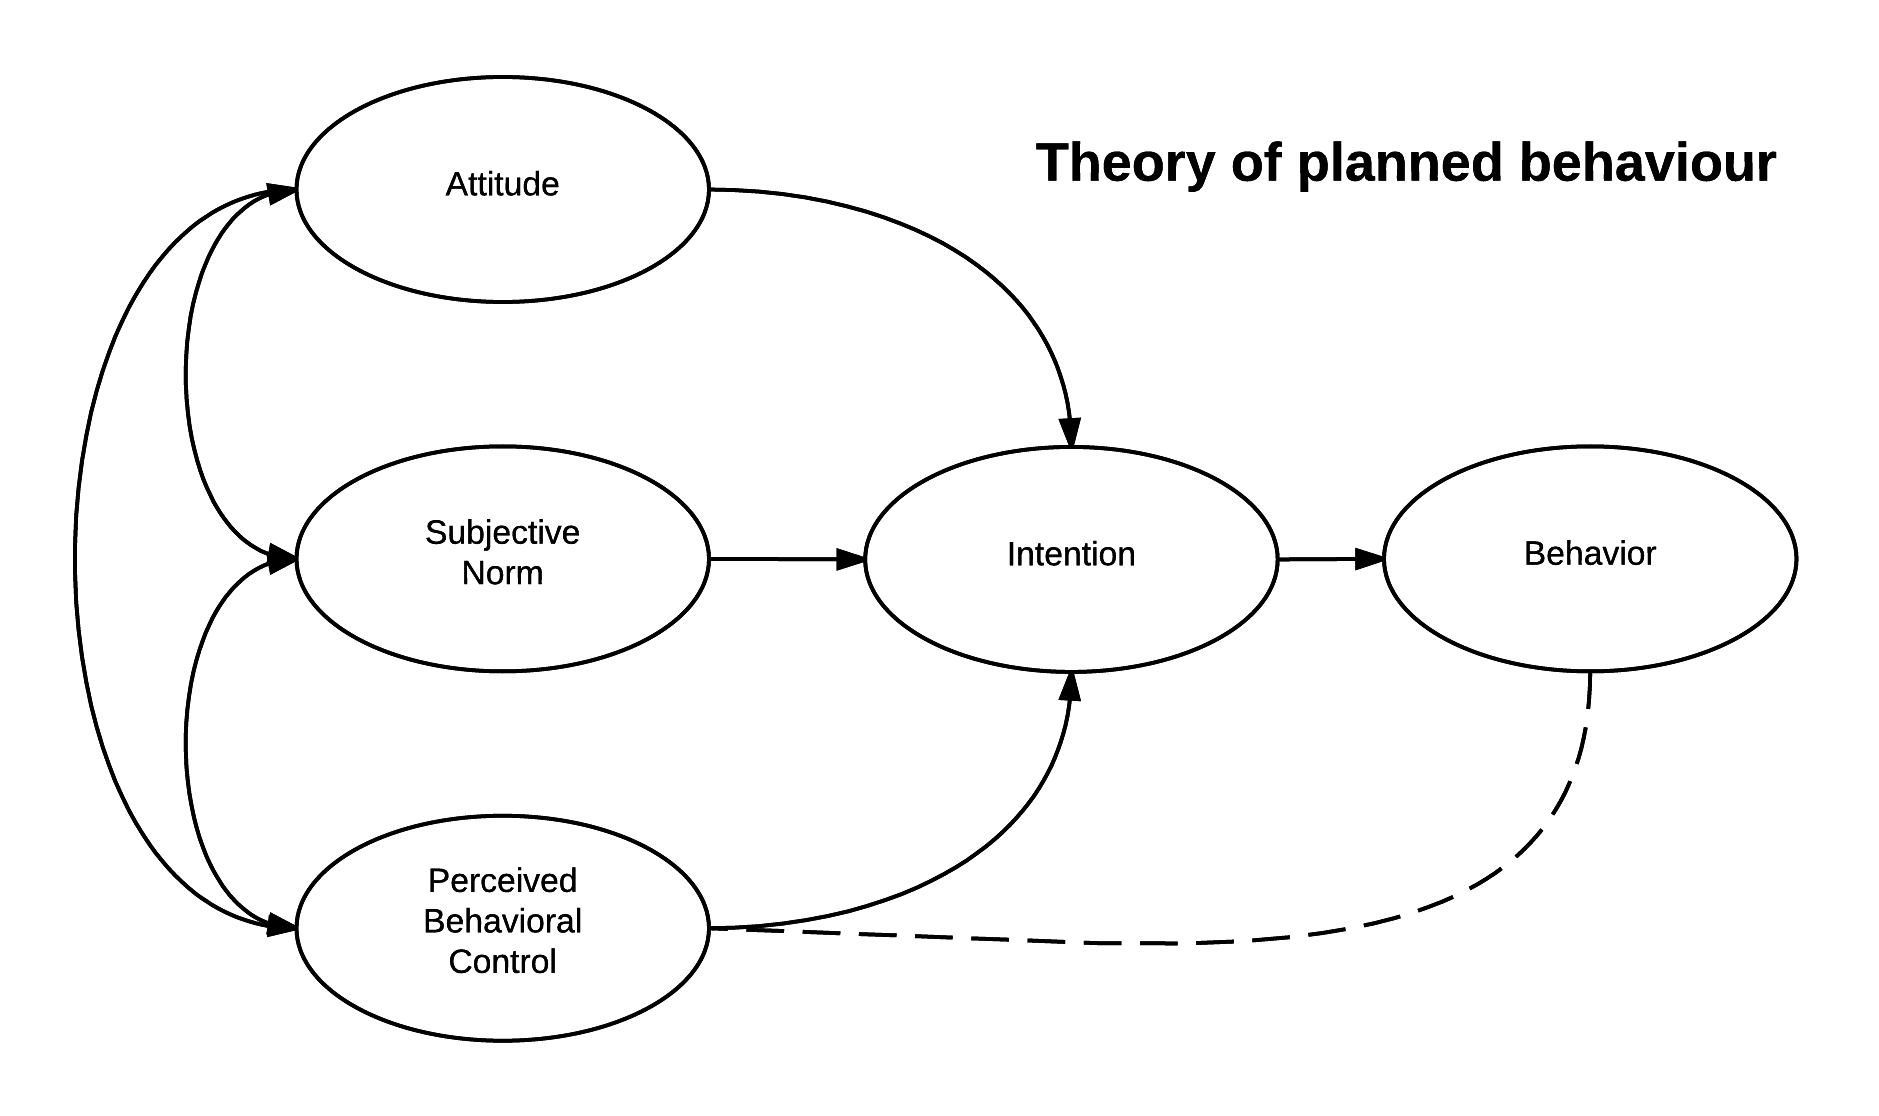
\includegraphics[width=0.8\textwidth]{Theory_of_planned_behavior_chart}}
    \caption{ساختار نظریه رفتار برنامه ریزی شده
      %\cite{kim2016integrated}
    }
    \label{fig:Theory_of_planned_behavior_chart}
  \end{figure}\\

  این نظریه در پژوهش‌های پیشین برای بررسی رفتار
  به اشتراک گذاری داده های خصوصی
  فرد در شبکه اجتماعی فیسبوک استفاده شده است
  \!\cite{vanderschyffInformationPrivacyBehavior2020}
  \!.
  مدلی که
  \!\gls{Theory of planned behavior}
  ارائه پیشنهاد می‌دهد، احتمال وقوع  رفتار‌های ارادی مخصوصا رفتار‌های ارادی مثبت به شدت تمایل فرد به
  انجام آن رفتار بستگی دارد.
  \!({\gls{Icek Ajzen}})
  عامل تعیین کننده برای انجام یک کار تمایلات او است.
\fi
%%%%%%%%%%%%%%%%%%%%

\ifSurveyfillingBehavior
  % بررسی اینکه آیا از نحوه پر کردن فرم ها می توان به کانفیدنس صداقت آزمودنی پی برد یا نه
  در صورتیکه گزینه‌های پرسشنامه اجباری باشند کیفیت داده‌های جمع‌آوری شده کاهش می یابد.
  \!\cite{sischkaImpactForcedAnswering2022}
\fi
% ^ %%%%%%%%%%%%%%%%%%%%%%%%%%%%%%%%%%%%%%%%%%%%%%%%%%%%%%%%%%%%%
% ^ %%%%%%%%%%%%%%%%%%%%%%%%%%%%%%%%%%%%%%%%%%%%%%%%%%%%%%%%%%%%%
% ^ %%%%%%%%%%%%%%%%%%%%%%%%%%%%%%%%%%%%%%%%%%%%%%%%%%%%%%%%%%%%%
\section{اهمیت}
%% توضیح بیشتر اضافه گردد بعدا
پژوهش انجام شده در سال ۲۰۲۰ نشان می دهد که در بازار داده های خصوصی آنلاین بازیگران زیادی به عنوان واسطه وجود دارند.
\!\cite{agogoInvisibleMarketOnline2021}
همچنین با گسترش هر روزه سیستم های اطلاعاتی که به
جمع‌آوری، ذخیره‌سازی، پردازش و به‌اشتراک‌گذاری داده‌های
خصوصی افراد می‌پردازند بررسی فرایندهای
تصمیم گیری و پارامتر‌های تاثیر گذار
بر این تصمیم‌گیری دارای اهمیت شده است
\!.
\!\cite{spiekermannValuesEthicsInformation2022}
از سوی دیگر نگرش افراد تصمیم گیرنده نسبت به ارزش اطلاعات خصوصی افراد می تواند نقش مهمی در رفتار آنها داشته باشد.
پژوهش‌هایی برای اندازه‌گیری ارزش داده‌های خصوصی انجام شده است
\!\cite{  fastValuePersonalData2021a,wesselsSellNotSell2019,tangHowChineseWeb2021}
\ifWillingnessToPay
  مقایسه میان رفتار افراد در پژوهش‌های اندازه‌گیری
  \textit{تمایل به پرداخت}
  \LTRfootnote{willingness to pay}
  نشان داده است که
  \textit{تمایل به پرداخت }
  با استفاده از روش‌های فرضی مانند
  \textit{ارزشيابی مشروط}
  \LTRfootnote{contingent valuation }
  میان ۱۷ تا ۶۳ درصد بالاتر
  از روشهای غیر فرضی مانند
  \textit{حراج تجربی}
  \LTRfootnote{experimental auction}
  است.
  حراج تجربی به عنوان یک روش
  \textit{سازگار با انگیزه}
  \LTRfootnote{incentive compatibility}
  شناسایی شده‌است
  \!\citep{martinez-carrascoComparingHypotheticalNonhypothetical2015}
  .
  یک فرایند،
  \textit{سازگار با انگیزه}
  است وقتی‌که همه شرکت‌کنندگان فقط  با درنظر گرفتن ترجیهات واقعی خود، بهترین خروجی را بدست می‌آورند
  \!\citep{nisanAlgorithmicGameTheory2007}
  \!.


\fi
% ^ %%%%%%%%%%%%%%%%%%%%%%%%%%%%%%%%%%%%%%%%%%%%%%%%%%%%%%%%%%%%%
% ^ %%%%%%%%%%%%%%%%%%%%%%%%%%%%%%%%%%%%%%%%%%%%%%%%%%%%%%%%%%%%%
% ^ %%%%%%%%%%%%%%%%%%%%%%%%%%%%%%%%%%%%%%%%%%%%%%%%%%%%%%%%%%%%%

\section{فرضیه پژوهشی}

% ^ %%%%%%%%%%%%%%%%%%%%%%%%%%%%%%%%%%%%%%%%%%%%%%%%%%%%%%%%%%%%%
% ^ %%%%%%%%%%%%%%%%%%%%%%%%%%%%%%%%%%%%%%%%%%%%%%%%%%%%%%%%%%%%%
% ^ %%%%%%%%%%%%%%%%%%%%%%%%%%%%%%%%%%%%%%%%%%%%%%%%%%%%%%%%%%%%%

% کلیه فایل‌های لازم برای حروف‌چینی با کلاس فوق، داخل پوشه‌ای به نام
% \lr{tehran-thesis}
% قرار داده شده است. توجه داشته باشید که برای استفاده از این کلاس باید فونت‌های
% \lr{IRLotusICEE}
% و
% \lr{IRTitr}
% را داشته باشید (که همراه با این کلاس هست و نیاز به نصب نیست).
% قلم‌های
% \lr{IRLotusICEE}
% مستخرج از قلم‌های استاندارد
% \lr{IRLotus}
% شورای عالی اطلاع‌رسانی%
% \footnote{
% قلم‌های استاندارد
% \lr{IRFonts}
% از شورای عالی اطلاع‌رسانی، منطبق بر آخرین نسخه استاندارد یونیکد، استاندارد ملی ۶۲۱۹ و استاندارد
% \lr{Adobe Glyph Naming}
% هستند.
% }
% هستند که توسط دکتر بابایی‌زاده اصلاحاتی روی آنها صورت پذیرفته است: تبدیل صفر توپر به صفر توخالی (جهت تمایز بیشتر با نقطه) و اضافه شدن
% \textit{\textbf{حالت توپر و ایرانیک توأم}}،
% که این موارد در قلم‌های شورای عالی اطلاع‌رسانی وجود ندارد.

% \subsection{این همه فایل؟!}
% \label{muchFiles}
% از آنجایی که یک پایان‌نامه یا رساله، یک نوشته بلند محسوب می‌شود، لذا اگر همه تنظیمات و مطالب پایان‌نامه را داخل یک فایل قرار بدهیم، باعث شلوغی و سردرگمی می‌شود. به همین خاطر، قسمت‌های مختلف پایان‌نامه یا رساله  داخل فایل‌های جداگانه قرار گرفته است. مثلاً تنظیمات پایه‌ای کلاس داخل فایل
% \lr{tehran-thesis.cls}، 
% قسمت مشخصات فارسی پایان‌نامه داخل 
% \lr{faTitle.tex}،
% مطالب فصل اول داخل 
% \lr{chapter1.tex}
% و تنظیمات قابل تغییر توسط کاربر داخل 
% \lr{commands.tex}،
% قرار داده شده است.
% \textbf{
% 	فایل اصلی این مجموعه، فایل
% 	\lr{main.tex}
% 	می‌باشد.
% }
% % یعنی بعد از تغییر فایل‌های دیگر، برای دیدن نتیجه تغییرات، باید این فایل را اجرا کرد. بقیه فایل‌ها به این فایل، کمک می‌کنند تا بتوانیم خروجی کار را ببینیم.
% اگر به فایل 
% \lr{main.tex}
% دقت کنید، متوجه می‌شوید که قسمت‌های مختلف پایان‌نامه، توسط دستورهایی مانند 
% \lr{input}
% و
% \lr{include}
% به فایل اصلی، یعنی 
% \lr{main.tex}
% معرفی شده‌اند.
% با توجه به ساختار محتوایی دستورالعمل، در فایل
% \lr{main.tex}
% فرض شده که پایان‌نامه یا رساله شما، از ۵ فصل و تعدادی پیوست تشکیل شده است. با اینحال، شما می‌توانید به راحتی فصل‌ها و پیوست‌ها را با صلاحدید اساتید راهنما، کم و زیاد کنید. این کار، بسیار ساده است. فرض کنید بخواهید یک فصل دیگر هم به پایان‌نامه اضافه کنید. برای این کار، کافی است یک فایل با نام دلخواه مثلاً 
% \lr{chapter6}
% و با پسوند 
% \lr{.tex}
% بسازید و آن را داخل پوشه 
% \lr{tehran-thesis}
% قرار دهید و سپس این فایل را با دستور 
% \verb!\include{chapter6}!
% داخل فایل
% \lr{main.tex}
%  فراخوانی کنید.

% \subsection{از کجا شروع کنم؟}
% قبل از هر چیز، باید یک توزیع تِک مناسب مانند تک‌لایو
% \lr{(TeXLive)}
% را روی سیستم خود نصب کنید. تک‌لایو  را می‌توانید از 
%  \href{http://www.tug.org/texlive}{سایت رسمی آن}%
% \LTRfootnote{\lr{\url{http://www.tug.org/texlive}}}
%  دانلود کنید یا مستقیماً از مخازن توزیع لینوکس خود بگیرید (مثلاً در اوبونتو با دستور
% \LRE{\verb!sudo apt install texlive-full!}).
% برای نصب تک‌لایو و اجرای اسناد زی‌پرشین می‌توانید از
% \href{http://parsilatex.com/site/shop/}{دی‌وی‌دی مجموعه پارسی‌لاتک}%
% \LTRfootnote{\lr{\url{http://parsilatex.com/site/shop/}}}
% و فایل راهنمای موجود در آن هم کمک بگیرید.

% برای تایپ و پردازش اسناد لاتک باید از یک ویرایشگر مناسب استفاده کنید. ویرایشگرهای
% \lr{TeXWroks},
% \lr{TeXstudio},
% \lr{Texmaker}
% و
% \lr{BiDiTeXmaker}
% بدین منظور تولید شده‌اند. می‌توان ویرایش‌گر 
%  \href{https://bitbucket.org/srazi/biditexmaker3}{\lr{BiDiTeXmaker}}%
%  \LTRfootnote{\lr{\url{https://bitbucket.org/srazi/biditexmaker3}}}
% را که بویژه برای کار با زی‌پرشین و مطالب دوجهته بهبود یافته است، بهینه‌ترین ویرایشگر لاتک برای کار با اسناد فارسی عنوان کرد.

% حال اگر نوشتن \پ اولین تجربه شما از کار با لاتک است، توصیه می‌شود که یک‌بار به صورت اجمالی، کتاب «%
% \href{http://www.tug.ctan.org/tex-archive/info/lshort/persian/lshort.pdf}{مقدمه‌ای نه چندان کوتاه بر
% \lr{\LaTeXe}}%
% \LTRfootnote{\lr{\url{http://www.tug.ctan.org/tex-archive/info/lshort/persian/lshort.pdf}\hfill}}»
% ترجمه دکتر مهدی امیدعلی را مطالعه کنید. این کتاب، کتاب بسیار کاملی است که خیلی از نیازهای شما در ارتباط با حروف‌چینی را برطرف می‌کند.
% اگر تک لایو کامل را داشته باشید، این کتاب را هم دارید. کافیست در خط فرمان دستور زیر را بزنید:
% \begin{latin}
% 	\texttt{texdoc lshort-persian}
% \end{latin}
% اگر عجله دارید، برخی دستورات پایه‌ای مورد نیاز در پیوست \ref{app:latexIntro} بیان شده‌اند.

% بعد از موارد گفته شده، فایل 
% \lr{main.tex}
% و
% \lr{faTitle.tex}
% را باز کنید و مشخصات پایان‌نامه خود مثل نام، نام خانوادگی، عنوان پایان‌نامه و ... را جایگزین مشخصات موجود در فایل
% \lr{faTitle.tex}
%  کنید. نیازی نیست نگران چینش این مشخصات در فایل پی‌دی‌اف خروجی باشید، زیرا کلاس 
% \lr{tehran-thesis}
% همه این کارها را بطور خودکار برای شما انجام می‌دهد. در ضمن، موقع تغییر دادن دستورهای داخل فایل
% \lr{faTitle.tex}
%  کاملاً دقت کنید؛ این دستورها، خیلی حساس هستند و ممکن است با یک تغییر کوچک، موقع اجرا، خطا بگیرید. برای دیدن خروجی کار، فایل 
% \lr{faTitle.tex}
%  را 
% \lr{Save}
% (نه 
% \lr{Save As})
% کنید و بعد به فایل 
% \lr{main.tex}
% برگشته و آن را اجرا کنید%
% \footnote{
% 	البته فایلهای این مجموعه به گونه‌ای هستند که در
% 	\lr{TeXWorks} یا
% 	\lr{TeXstudio}
% 	بدون بازگشت به فایل اصلی، می‌توانید سند خود را اجرا کنید.
% }.
%  حال اگر می‌خواهید مشخصات انگلیسی \پ را هم عوض کنید، فایل 
% \lr{enTitle.tex}
% را باز کنید و مشخصات داخلش را تغییر دهید.
% %\RTLfootnote{
% %برای نوشتن پروژه کارشناسی، نیازی به وارد کردن مشخصات انگلیسی پروژه نیست. بنابراین، این مشخصات بطور خودکار، نادیده گرفته می‌شود.
% %}
% در اینجا هم برای دیدن خروجی باید این فایل را ذخیره کرده، بعد به فایل 
% \lr{main.tex}
% برگشته و آن را اجرا کرد.

% برای راحتی بیشتر، کلاس 
% \lr{tehran-thesis.cls}
% طوری طراحی شده است که کافی است فقط  یک‌بار مشخصات \پ را (در فایل‌های
% \lr{faTitle.tex}
% و
% \lr{enTitle.tex})
% وارد کنید و هر جای دیگر که این مشخصات لازم باشند، به طور خودکار درج می‌شوند. با این حال، اگر مایل بودید، می‌توانید تنظیمات موجود را تغییر دهید؛ گرچه، در صورتیکه کاربر مبتدی هستید و یا با ساختار فایل‌های  
% \lr{cls}
%  آشنایی ندارید، بهتر است به فایل 
% \lr{tehran-thesis.cls}
% دست نزنید.

% نکته دیگری که باید به آن توجه کنید این است که در قالب آماده شده، سه گزینه به نام‌های
% \lr{bsc}،
% \lr{msc}
% و
% \lr{phd}
% برای نوشتن پروژه، پایان‌نامه و رساله، در نظر گرفته شده است. بنابراین اگر قصد تایپ پروژهٔ کارشناسی، پایان‌نامهٔ کارشناسی ارشد یا رسالهٔ دکتری را دارید، به ترتیب باید از گزینه‌های
% \lr{bsc}،
% \lr{msc}
% و
% \lr{phd}
% در فایل 
% \lr{main.tex}
% استفاده کنید. با انتخاب هر کدام از این گزینه‌ها، تنظیمات مربوط به آنها به طور خودکار، اعمال می‌شود.


% \subsection[مطالب پایان‌نامه را چطور بنویسم؟]
% {مطالب \پ را چطور بنویسم؟}
% \subsubsection{نوشتن فصل‌ها}
% همان‌طور که در بخش \ref{muchFiles} گفته شد برای جلوگیری از شلوغی، قسمت‌های مختلف \پ از جمله فصل‌ها، در فایل‌های جداگانه‌ای قرار داده شده‌اند. 
% مثلاً اگر می‌خواهید مطالب فصل ۱ را تایپ کنید، باید فایل‌های 
% \lr{main.tex}
% و
% \lr{chapter1.tex}
% را باز کرده و مطالب خود را جایگزین محتویات داخل 
% \lr{chapter1.tex}
% نمایید. دقت شود که در ابتدای برخی فایلها دستوراتی نوشته شده است و از شما خواسته شده که آن دستورات را حذف نکنید.

%توجه کنید که همان‌طور که قبلاً هم گفته شد، تنها فایل قابل اجرا، 
%\lr{main.tex}
%است. لذا برای دیدن حاصل (خروجی) فایل خود، باید  
%\lr{chapter1.tex}
%را ذخیره کرده و سپس فایل 
%\lr{main.tex}
%را اجرا کنید.

% نکته بسیار مهمی که در اینجا باید گفته شود این است که سیستم \lr{\TeX}، محتویات یک فایل تِک را به ترتیب پردازش می‌کند.  بنابراین، اگر مثلاً  دو فصل اول خود را نوشته و خروجی آنها را دیده‌اید و مشغول تایپ مطالب فصل ۳ هستید، بهتر است
% که دو دستور 
% \verb!% !TeX root=main.tex
% دستور زیر باعث شماره‌بندی صفحات فصول از ۱ می‌شود و باید در اولین فصل شما باشد. آن را حذف نکنید!
\pagenumbering{arabic} % 1, 2, ...

\chapter{مقدمه}
% دستور زیر باعث عدم‌نمایش شماره صفحه در اولین صفحه‌ی این فصل می‌شود.
%\thispagestyle{empty}
\ifDataveillance
  \textit{کریستین فوکس}
  \LTRfootnote{Christian Fuchs}
  جامعه شناس اتریشی،
  \textit{
    \gls{Social networking service}
  }
  \!({\lr{SNS}})
  در دنیای مدرن را به یک
  \textit{
    \gls{Panopticon}
  }
  تشبیه می کند   که در آن شرکت‌های بزرگی مانند
  \textit{
    \gls{Alphabet}
  }
  \!(
  شرکت مادر سرویس
  \textit{
    \gls{Google}
  }
  \!)
  و
  \textit{
    \gls{Meta}
  }
  \!(
  \!شرکت مادر و مالک برنامه‌های نرم‌افزاری مانند
  \textit{
    \gls{Instagram}
  }،
  \textit{
    \gls{Facebook}
  }
  و
  \textit{
    \gls{Whatsapp}
  }
  \!)
  به
  \textit{
    \gls{Dataveillance}
  }
  اعضا می‌پردازند
  \!\citep{romelePanopticismNotEnough2017a}.
  عبارت
  \textit{
    \gls{Panopticon}
  }
  را اولین بار
  \textit{
    \gls{Jeremy Bentham}
  }
  \!
  \citep{benthamPanopticonInspectionHouseContaining1791}
  برای توصیف ساختار‌های اجتماعی که مانند سیستم متمرکز نظارت عمل می‌کنند، از معماری وارد
  \textit{
    \gls{Social philosophy}
  }
  کرد.
\fi %Dataveillance
% * from old proposal and thesis fron khordad 1400 /media/d_drive/PJ/K/C/PJ-HDD-NiliLab/ssd2-laptop-backup-4mordad00/PJ/KN/Cog/proposal/tex/003
به نظر می‌رسد تصمیم‌گیرندگانی که در چنین سازمان‌هایی حضور دارند به حجم زیادی از اطلاعات
شخصی افراد دسترسی دارند. چنین افرادی، به علت وظیفه‌ای که در قبال سازمان
متبوع خود دارند، ملزم با حداکثر کردن سود بنگاه‌های اقتصادی هستند
که مالکیت این سازمان‌ها و سرویس‌های ارائه شده را، در اختیار
دارند.از طرف دیگر، همین تصمیمات می‌تواند باعث متضرر شدن
کاربرانی باشد که مالک اصلی اطلاعات جمع‌آوری شده می‌باشند. در چنین شرایطی، وقتی که
\textit{
  \glspl{Oversight institution}
}
با تغییرات سریع  در ساختارهای
\textit{
  \glspl{Information society}
}
ناهماهنگ هستند
\!\citep{cavoukianDiscussionPaperPrivacy2009,machovaDiscourseSurveillancePrivacy2021}،
بررسی ساز و کار موثر بر تصمیمات این افراد، اهمیت پیدا می‌کند.
اهمیت  این موضوع زمانی بیشتر می‌شود که کاربران
\textit{
  \gls{Social networking service}
}
تحت تاثیر
\textit{
  \glspl{Motivitions of}
}
متضاد قرار می‌گیرند و رفتاری را نشان می‌دهند که با عنوان
\textit{
  \gls{Privacy paradox}
}
شناخته می‌شود
\!citep{barthPrivacyParadoxInvestigating2017}.

این رفتار زمانی مشاهده می‌شود که کاربران شبکه‌های اجتماعی با وجود اهمیتی که برای حفظ
\textit{
  \gls{Information privacy}
}
بیان می‌کنند باز هم بی‌محابا نسبت به  منتشر کردن اطلاعات شخصی خود
در شبکه‌های اجتماعی اقدام می‌کنند.

این رفتار حتی پس از آگاه شدن از
پیامدهای سوءاستفاده از این اطلاعات نیز کاهش چشمگیری نداشته است
\!\citep{hermesWhoQuitsPrivacyInvasive2021,wirthLazinessExplanationPrivacy2022}.
به نظر می‌رسد که جلوگیری از پیامدهای  نامطلوب سوءاستفاده از اطلاعات خصوصی کاربران و نقض
\textit{
  \gls{Information privacy}
}
از طریق مداخلاتی که در سطح کاربران انجام شود، با توجه به گسترش و تنوع جمعیتی،
دشوار خواهد بود. با این وجود،
\textit{
  \gls{Information privacy}
}
که به توانایی افراد
برای کنترل اطلاعات مربوط به آنها اشاره دارد
\!{\cite{smithInformationPrivacyMeasuring1996}}
در سال‌های اخیر بیشتر مورد توجه کاربرانی قرار گرفته است
که داده‌های آنها توسط
\textit{
  \glspl{Social networking service}
}
جمع‌آوری، طبقه‌بندی و تحلیل می شود
\!{\cite{wallOrganizationalViolationsExternally2016}}
\!.
\textit{
  \gls{Information privacy}
}
با اشتراک‌گذاری اطلاعات شخصی توسط صاحب اطلاعات، در تضاد نیست.
\textit{
  \gls{Information privacy}
}
داشتن کنترل بر روی اطلاعات بعد از به  اشتراک‌گذاری، می‌باشد.
\!{\cite{acquistiEconomicsPrivacy2016}}.
به اشتراک گذاری اطلاعات شخصی از دید صاحبان اولیه اطلاعات،
به عنوان یک رفتار اجتماعی ناخوشایند و بالقوه ناهنجار، شناسایی شده است،
\!{\cite{norbergCopingInformationRequests2014}}،
اما به نظر می‌رسد چنین دیدگاهی با تعریفی که برای
\textit{
  \gls{Information privacy}
}
ارائه شد، در تضاد قرار می‌گیرد. اگر کاربران بتوانند بعد از
\textit{
  \gls{Disclosure}
}
اطلاعات خود، بر روی نحوه استفاده از آن کنترل داشته باشند،
\textit{
  \gls{Personal Information Sharing Behavior}
}
به تنهایی
اثرات مخربی در پی نخواهد داشت.  به علاوه
جمع‌آوری و پردازش اطلاعات می‌تواند نتایج سازنده‌ای، در سطح
اجتماعی و فردی داشته باشد
\!\citep{rockenbachProvidingPersonalInformation2020}.
افرادی که در
\textit{
  \glspl{Information society}
}
فاقد
\textit{
  \glspl{information record}
}
کافی در
\textit{
  \gls{Big data}
}
باشند، از جهات مختلف مورد
\textit{
  \gls{Discrimination}
}
قرار می‌گیرند
\!\citep{favarettoBigDataDiscrimination2019,lermanBigDataIts2013}.
با این دیدگاه، به اشتراک گذاری اطلاعات شخصی توسط صاحب اطلاعات، نه تنها
ناسازگارانه نیست، بلکه به یک رفتار
\textit{
  \gls{Prosocial}
}
تبدیل می‌شود. اطلاعات کاربران پس از
\textit{
  \gls{Disclosure}
}
در اختیار تصمیم‌گیرندگانی قرار می‌گیرد که در
\textit{
  \glspl{Social networking service}
}
مسئول جمع‌آوری، ذخیره‌سازی و پردازش اطلاعات هستند. به نظر می‌آید که حفظ
\textit{
  \gls{Information privacy}
}
و جلوگیری از اثرات مخرب اجتماعی و فردی سوءاستفاده از
اطلاعات شخصی انباشته شده، از طریق شناسایی عوامل موثر
بر تصمیم‌گیری این افراد و به اجرا در آوردن
مداخلات موثر در این سطح،نتایج بهتری در پی داشته باشد.

کاربران
\textit{
  \glspl{Social networking service}
}
پس از ارائه اطلاعات شخصی خود، خدماتی را از آن دریافت می‌کنند. این
تبادل میان کاربر و
\textit{
  \glspl{Social networking service}
}
مورد توافق طرفین است. شرایط حاکم بر این تبادل در توافق‌نامه‌ای
که در زمان عضویت به افراد ارائه می‌شود، مشخص شده است. به عنوان مثال
فرد در قبال اطلاعات شخصی خود از امکانات
\textit{
  \glspl{Social networking service}
}
برای برقراری ارتباط با دوستان خود استفاده می کند. او همچنین
با شروط دیگری که  برای عضویت لازم بوده است، موافقت کرده است. او
قبول کرده است که
\textit{
  \gls{Social networking service}
}
اطلاعات شخصی‌اش را در جهت ارائه تبلیغات هدفمند به کاربران، ذخیره کند
و مورد بازبینی و پردازش قرار دهد. اثرات مخرب این تبادل از زمانی شروع می شود که دریافت کننده اطلاعات، از
آن برای اهدافی به غیر از توافق اولیه استفاده کند و یا امکان این کار را برای یک شخص ثالث فراهم کند
\!{\cite{padyabExploringImpactsSecondary2018}}.

\textit{
  \gls{Secondary use of information}
}،
استفاده از اطلاعات شخصی برای اهدافی فراتر
از توافق اولیه، بعد از
\textit{
  \gls{Disclosure}
}
اطلاعات شخصی فرد، است. این عمل توسط موسسه جمع‌آوری کننده اطلاعات
و افراد تصمیم‌گیرنده در آن انجام می‌گیرد
\!{\cite{culnanHowDidThey1993}}.
پیامد‌های زیانبار تصمیمات بنگاه‌های اقتصادی و فن‌آوری بزرگی
مانند
\textit{
  \glspl{Meta}
}
برای استفاده ثانویه از اطلاعات شخصی جمع‌آوری شده، در پژوهش‌های مختلف بررسی شده اند
\!{\cite{padyabExploringImpactsSecondary2018}}.
این تصمیمات در سال‌های ۲۰۱۵ تا ۲۰۱۸، منجر به ناهنجاری‌های وسیع در سطح جوامع شدند
\!{\cite{redmanDataCredibilityProblem2013,dezwartSurveillanceBigData2014,spiekermannNetworksControlReport2016,schyffDuplicitouslMedia2020}}.
پیامدهای این ناهنجاری‌ها در نهایت افراد عضو جوامع را به طور غیر مستقیم
تحت تاثیر قرار می‌دهند. این افراد، متشکل از همان کاربرانی هستند که به طور جمعی، تامین کننده
داده‌های جمع‌آوری شده توسط
\textit{
  \glspl{Meta}
}
بوده‌اند.
\!{\cite{redmanDataCredibilityProblem2013,dezwartSurveillanceBigData2014,spiekermannNetworksControlReport2016,schyffDuplicitouslMedia2020}}.
با وجود آسیب‌پذیری افراد از داده‌های شخصی جمع‌آوری شده توسط شرکت‌ها
و شرکای تجاری آنها، تحقیقات نشان می‌دهد
که کاربران این جنبه تبادل اطلاعات خود را نادیده می‌گیرند
\!{\cite{raynes-goldieAliasesCreepingWall2010,brandtzaegTooManyFacebook2010,youngPrivacyProtectionStrategies2013}}،
هرچند با توجه به تاثیرات سازنده‌ای که برای رفتار اشتراک گذاری اطلاعات در بخش‌های
قبلی نام برده شده است، به نظر می‌رسد که می‌توان، تغییرات نامحسوس رفتار کاربران در
\textit{
  \gls{post–Cambridge Analytica scandal era}
}
\!{\citep{epsteinViewFramingDigital2021}}
را، پدیده مطلوبی توصیف کرد. با این وجود وقوع چنین پدیده‌هایی به 
\textit{
  \gls{Trust}
}
 در افراد جامعه آسیب می‌زند و در نهایت سبب کاهش منافع جمعیِ جمع‌آوری و پردازش اطلاعات، می‌گردد.


\gls{Cambridge Analytica scandal}
در سال ۲۰۱۶ باعث پی‌گیری‌ حقوقی شرکت 
\glspl{Meta} 
و مدیرعامل آن 
\textit{
  \gls{Mark Zuckerberg}
}
و محکومیت به پرداخت جریمه پنج میلیارد دلاری، شد
.\!{\citep{daviesFacebookPay5bn2019m,FacebookAgreesPay2019}}
واکنش مسؤولین فیسبوک نشان می‌دهد
که افراد تصمیم گیرنده در شرکت‌های جمع‌آوری کننده
اطلاعات نیز احتمالا از پیامدهایی که سیاست‌گذاری‌های آنها در استفاده ثانویه از اطلاعات شخصی کاربران
برای خود شرکت در پی دارد، ناآگاه هستند
\!{\cite{SuspendingCambridgeAnalytica2018,FacebookDataPrivacy2018}}
\!. با توجه به اینکه این افراد مسؤول حداکثر
کردن سود شرکت‌های خود هستند،
به نظر می‌رسد که چنین تصمیماتی فرض
\glspl{Rational}
بودن عامل‌های تصمیم‌گیرنده را در
\glspl{Rational choice theory}
به چالش می‌کشد. با در نظر گرفتن این مساله‌، ما در این پژوهش از از یک چارچوب نظری که فرض
\textit{
  \gls{Rational}
}
بودن تصمیمات را به چالش می‌کشند برای
\textit{
  \glspl{Articulation}
}
مفاهیم و رویکردهایمان استفاده کردیم.


تحقیقات زیادی برای بررسی رفتار کسانی که
اطلاعات خود را در اینترنت به اشتراک می‌گذارند انجام شده است
\!\!{\cite{kamleitnerInformationSharingPrivacy2019,kamleitnerYourDataMy2019}}.
همچنین رفتار افرادی که در مالکیت اطلاعت با فرد دیگر، شریک هستند بررسی شده است
\!\!{\cite{tawnieInterdependentPrivacy2017}}.
نتایج نشان می‌دهد که با وجود اینکه در همه جهان
\!،
\textit{
  \gls{Privacy}
}
اطلاعات شخصی افراد مساله مهمی برای کاربران آنلاین
است، بیشتر کاربران به ندرت برای محافظت از این داده، به خود زحمت می‌دهند و حتی در
بیشتر مواقع به طور داوطلبانه آن‌را پخش می‌کنند. تلاش زیادی انجام شده است تا این
دوگانگی میان
\textit{
  \gls{Privacy Attitude}
}
و رفتار، که معمولا با عنوان
\textit{
  \gls{Privacy paradox}
}
شناخته می‌شود، توضیح داده شود
\!\!{\cite{gerberExplainingPrivacyParadox2018}}.
به طور مشابه پژوهشی که در زمینه رفتار
\textit{
  \gls{Trust}
}
با به کار بردن
\textit{
  \gls{Theory of planned behavior}
}
در
\textit{
  \gls{Trust game}
}
انجام شده است،  وجود چنین تناقضی را در افراد
\textit{
  \gls{Trustor}
}
نیز نشان می‌دهد
\!\cite{gazdagNotWantTrust2019}.
به طور کلی، تا کنون  تحقیقات زیادی در حوزه
\textit{
  \gls{Information privacy}
}،
از
\textit{
  \gls{Trust game}
}
برای بررسی رفتار افراد در این تعامل
\textit{
  \gls{Interpersonal}
}،
استفاده کرده اند. با وجود اینکه تا به امروز رفتار کاربرانی که اطلاعات
\!(یا اطلاعات مشترک)
خود را به اشتراک می‌گذارند، مورد کنکاش قرار گرفته است، حیطه
رفتاری افرادی که دریافت کننده این  اطلاعات هستند به ندرت
مورد توجه قرار گرفته است
\!\cite{demmersYourDataAre2021}.

\subsection{کمبریج آنالیتیکا و استفاده ثانویه از اطلاعات}
در سال ۲۰۱۳ استاد دانشگاه کمبریج یک برنامه به نام 
«\lr{thisisyourdigitallife}»
ساخت. این برنامه در شبکه اجتماعی فیسبوک به کاربران 
آزمون‌های شخصیت‌شناسی ارائه می‌کرد. وقتی کاربر فیسبوک برنامه را بر روی حساب کاربری خود فعال و نصب
می‌کرد، برنامه جمع‌آوری اطلاعات شخصی او را آغاز می‌کرد. این اطلاعات شامل اطلاعات حساب کاربری و فعالیت‌های کاربر در فیسبوک
بود. فعالیت‌هایی مانند اینکه کاربر کدام محتوای فیسبوک را لایک کرده است. در حدود سیصد هزار نفر این 
برنامه را نصب کردند. اما اطلاعاتی که جمع‌آوری شد به این تعداد محدود نماند.  
این برنامه اطلاعاتی درباره دوستان کاربر که تنظیمات حریم خصوصی خود را درست  تنظیم نکرده بودند، را 
نیز جمع‌آوری کرد. در نتیجه برنامه توانست اطلاعات ۸۷ میلیون نفر را جمع‌آوری کند
\!\cite{kangFacebookSaysCambridge}.

سپس دکتر کوگان داده چمع‌آوری شده را به شرکت 
\textit{
  \gls{ Strategic Communication Laboratories (SCL)}
}
که مالک شرکت کمبریج آنالیتیکا است، انتقال داد. این شرکت یک موسسه مشاوره
سیاسی بود که از داده برای شناسایی ویژگی‌های شخصیتی و رفتار رای دهندگان
استفاده می‌کرد
\!\cite{rosenbergHowTrumpConsultants2018}. 
این شرکت از این داده برای کمک به به پویش محافظه‌کاران برای هدف
قرار دادن تبلیغات اینترنتی و پیام رسان‌ها استفاده کرد. این همان عملی 
بود که دکتر کوان شرایط و مقررات فیبوک را نقض کرد که انتقال یا 
فروش داده به هر شبکه تبلیغاتی ، دلال داده یا هر سرویس تبلیغاتی 
و درآمد‌زایی، ممنوع می‌کرد
\!\cite{granvilleFacebookCambridgeAnalytica2018}. 

وقتی در سال ۲۰۱۵ فیسبوک از این موضوع مطلع شد، برنامه دکتر کوگان 
را حذف  کرد و از کوگان و کمبریج آنالیتیکا درخواست کرد که
مدرکی ارائه دهند، که داده را پاک کرده‌اند. کوگان و کمبریج آنالیتیکا
به فیسبوک تاییده‌ای ارائه دادند که داده را حذف کرده‌اند. هرچند  کپی داده
خارج از کنترل فیسبوک باقی ماند.  وقتی الکساندر نیکس، مدیر عامل
کمبریج آنالیتیکا، به قانون‌گذاران گفت که شرکتش داده‌های فیسبوک را در
اختیار ندارد، یکی از کارمندان گفت که او اخیرا صدها گیگابایت داده را
بر روی سرورهای کمبریج آنالیتیکا دیده‌است و اطلاعات رمز نگاری نشده بودند.

در سال ۲۰۱۵، فیسبوک هیچ بیانیه عمومی‌ای درباره این رخداد منتشر نکرد. همچنین
کاربرانی که اطلاعات‌شان با کمبریج آنالیتیکا به اشتراک گذاشته شده 
بود. همچنین فیسبوک به کمیته تجارت فدرال، درباره این موضوع
چیزی نگفت. بر اساس آنچه که مارک زاکربرگ در کنفرانس دو روزه
 استماع‌اش در نهم و دهم آوریل ۲۰۱۸ گفت، به محض اینکه گواهی کمبریج آنالیتیکا
 مبنی بر حذف و تعهد عدم استفاده از داده را دریافت کردند، فیسبوک
 موضوع را خاتمه یافته تلقی کرد
 \!\cite{spanFacebookCEOMark}. 

 با منتشر شن این داستان در مارس ۲۰۱۸ در دو نشریه بین‌المللی، فیسبوک
 مطلع شد که داده تا آن روز پاک نشده بوده است. نتایج به بار آمده
 چنین حادثه‌ای بی سابقه بود. فیسبوک توسط چند نهاد قضایی در ایالت متحده، 
 جزیره انگلستان و اتحادیه اروپا مورد بازخواست قضایی قرار گرفت. یک پویش
 فیسبوک را حذف کنید راه افتاد و افت شدید قیمت سهام باعث شد تقریبا پنجاه میلیارد دلار
 سرمایه شرکت در عرض سه روز پس از فاش شدن اخبار، از بین رفت.




%   \glspl{phenomenon of dyadic completion}
%   نشان می دهد که گرایش های
%   \glspl{deontological}
%   و
%   \glspl{utilitarian}
%   نه تنها به طور همزمان فعال هستند
%   بلکه اغلب سازگار و تقویت کننده می‌باشند
%   \!{\cite{grayTwoMindsVs2012}}.
\subsection{چارچوب‌های نظری}
\textit{
  \gls{Rational choice theory}
}
\!{\cite{beckerEconomicApproachHuman1978}}،
این فرض را بنا می‌نهد که انسان‌ها بر اساس
تابعی از مجموع منفعت، با کسر مجموع هزینه‌های یک تصمیم
یا مبادله و برای حداکثر کردن فایده  شخصی دست به عمل می‌زنند.

این موضوع پایه‌ای برای طرح نظریه
\textit{
  \gls{Theory of reasoned action}
}
توسط
\textit{
  \gls{Icek Ajzen}
}
و
\textit{
  \gls{Martin Fishbein}
}
در در دهه ۸۰ میلادی شد. این نظریات پیشنهاد می‌کنند که بین
\textit{
  \gls{Atteutude}
}
و رفتار رابطه وجود دارد
\!{\cite{ajzenPredictionGoaldirectedBehavior1986}}.
فهم رفتار اختیاری افراد به وسیله
بررسی انگیزه‌هایی که باعث اجرای یک عمل می شود، هدف اصلی این نظریه بود. این نظریه
بیان می کند که قصد اجرای یک عمل پیش‌بینی‌کننده اصلی انجام یا عدم ایجاد رفتار  است. به
علاوه پارامتر هنجاری
(هنجارهای اجتماعی که عمل را احاطه کرده‌اند)
در اجرا شدن یا نشدن عمل نقش بازی می کند
\!{\citep{HealthBehaviorTheory2015,doswellTestingTheoryReasoned2011,ajzenAttitudesAttitudeBehaviorRelation2000}}
.
اما تحقیقاتی که در قالب چارچوب‌های
\textit{
  \gls{Behavioral economics}
}
انجام شد، این فرض را مورد تردید قرار داده اند
\!\cite{henrichEconomicManCrosscultural2005}.
برای رفع کاستی‌های
\textit{
  \gls{Theory of reasoned action}
}
آیزن در سال ۱۹۹۱ 
\!\citep{ajzenTheoryPlannedBehavior1991}
\textit{
  \gls{Theory of planned behavior}
}
را مطرح کرد. به بیان این تئوری سه پارامتر اصلی
\textit{
  \gls{Attitude}
}
\!،
\textit{\gls{Subjective norm}}
و
\textit{\gls{Perceived Behavioral control}}
\!،
\textit{\glspl{Behavioral intention}}
افراد را شکل می‌بخشند. پایه تفکر
\textit{
  \gls{Theory of planned behavior}
}
این است که
\textit{
  \gls{Personal Information Sharing Behavior}
}
از تعامل
\textit{\glspl{Psychological construct}}
\textit{
  \gls{Attitude}
}
\!،
\textit{\gls{Subjective norm}}،
\textit{\gls{Perceived Behavioral control}}
و
\textit{\glspl{Behavioral intention}}
نسبت به 
\textit{
  \gls{Personal Information Sharing}
}،
ایجاد می‌شود. 

در پژوهش‌های پیشین برای بررسی
\textit{
  \gls{Personal Information Sharing Behavior}
}
از
\textit{
  \gls{Theory of reasoned action}
}
\!\citep{malhotraInternetUsersInformation2004}،
و
\textit{
  \gls{Theory of planned behavior}
}
برای ایجاد ساختاری که روابط بین پارامترها را مدل می‌کند، استفاده شده است
\!\citep{dinevExtendedPrivacyCalculus2006b}.

در این پژوهش ما بررسی رفتار به اشتراک گذاری اطلاعات خصوصی دیگران در
\textit{
  \gls{Conceptual framework}
}
\textit{
  \gls{Theory of planned behavior}
}
پرداختیم.

برای سنجش رویکرد‍ افراد به
\textit{
  \gls{Personal information of Others}
}
یک پرسشنامه بر اساس دسته‌بندی‌های هفت‌گانه‌ای که در پژوهش پیشین با توجه به رویکرد صاحبان
اولیه اطلاعات خصوصی نسبت به خطر فاش شدن اطلاعات شخصی شان در حوزه‌های مختلف، ساخته شد.
این پرسشنامه برای هر دسته از سوالات دارای ۲ سوال است. برای اینکه بتوان باور 
آزمودنی‌ها، را هم بر اساس ارزش ذهنی خود
\!(نگرش به ارزش اطلاعات)
و هم بر اساس ارزش ذهنی دیگران
\!(هنجار ذهنی و باور هنجاری)
و همچنین برای اندازه‌گیری پایایی درونی،
سوالات به دو دسته تقسیم ‌می‌شود.
به هر آزمودنی، دسته اول اطلاعات خصوصی به همراه یک سوال برای سنجش باور هنجاری، و دسته دوم
اطلاعات به همراه سوال دیگر برای سنجش باور شخصی، ارائه شد. به طور تصادفی این دو دسته از 
سوالات برای هر آزمودنی جابجا شدند تا در نهایت پاسخ‌های نیمی از آزمونی‌ها به دسته اول سوالات از دید خود و نیمی 
دیگر از آزمودنی ها به دسته دوم سوالات از دید خود، جمع‌آوری شوند. به همین ترتیب پاسخ به سوالات دسته اول و دوم 
با توجه به باور هنجاری از دو دسته مستقل به تصادف انتخاب شدند، جمع‌آوری شد. تصادفی سازی در زمان وردو آزمودنی‌ها
به آزمایش با انتصاب افراد با احتمال ۵۰ درصد به دو گروه، انجام شد.
% * %%%%%%%%%%%%%%%%%%%%%%%%%%%%%%%%%%%%%%%%%% from old proposal and thesis from khordad 1400

\section{متغیر‌ها و پرسشنامه‌ها}

\ifPlennedBahaviorTheory
  \textit{\gls{Theory of planned behavior}}
  \!(TPB)
  % \LTRfootnote{Theory of planned behavior (TPB) }
  %  acronyms اضافه شود
  ، تعامل سه باور فردی شامل
  \textit{\gls{Atteutude}} ،
  \textit{\gls{Subjective norm}} و
  \textit{\gls{Perceived Behavioral control}}
  % \LTRfootnote{Perceived Behavioral control}
  را عامل رفتار می داند
  \!(شکل: \ref{fig:Theory_of_planned_behavior_chart})
  \!\cite{ajzenTheoryPlannedBehavior2020}.
  در این نظریه 
  \textit{\gls{Atteutude}}
 از دو نگرش احساسی و نگرش ابزاری تشکیل شده است.
  \textit{\gls{Subjective norm}}
  شامل  هنجارهای ذهنی و هنجار توصیفی است.
  \textit{\gls{Perceived Behavioral control}}،
  دو بخش کنترل رفتاری درک شده و خود کارآمدی درک شده را شامل می باشد
  در این نظریه عامل اصلی تعیین کننده
  رفتار، قصد رفتاری است و اجزای ساختاری این نظریه
  بر روی قصد تاثیر ویژه‌ای دارند
  \cite{mhmdpwrBrrsyTthyrTywry2022}
  \begin{figure}[ht]
    \centerline{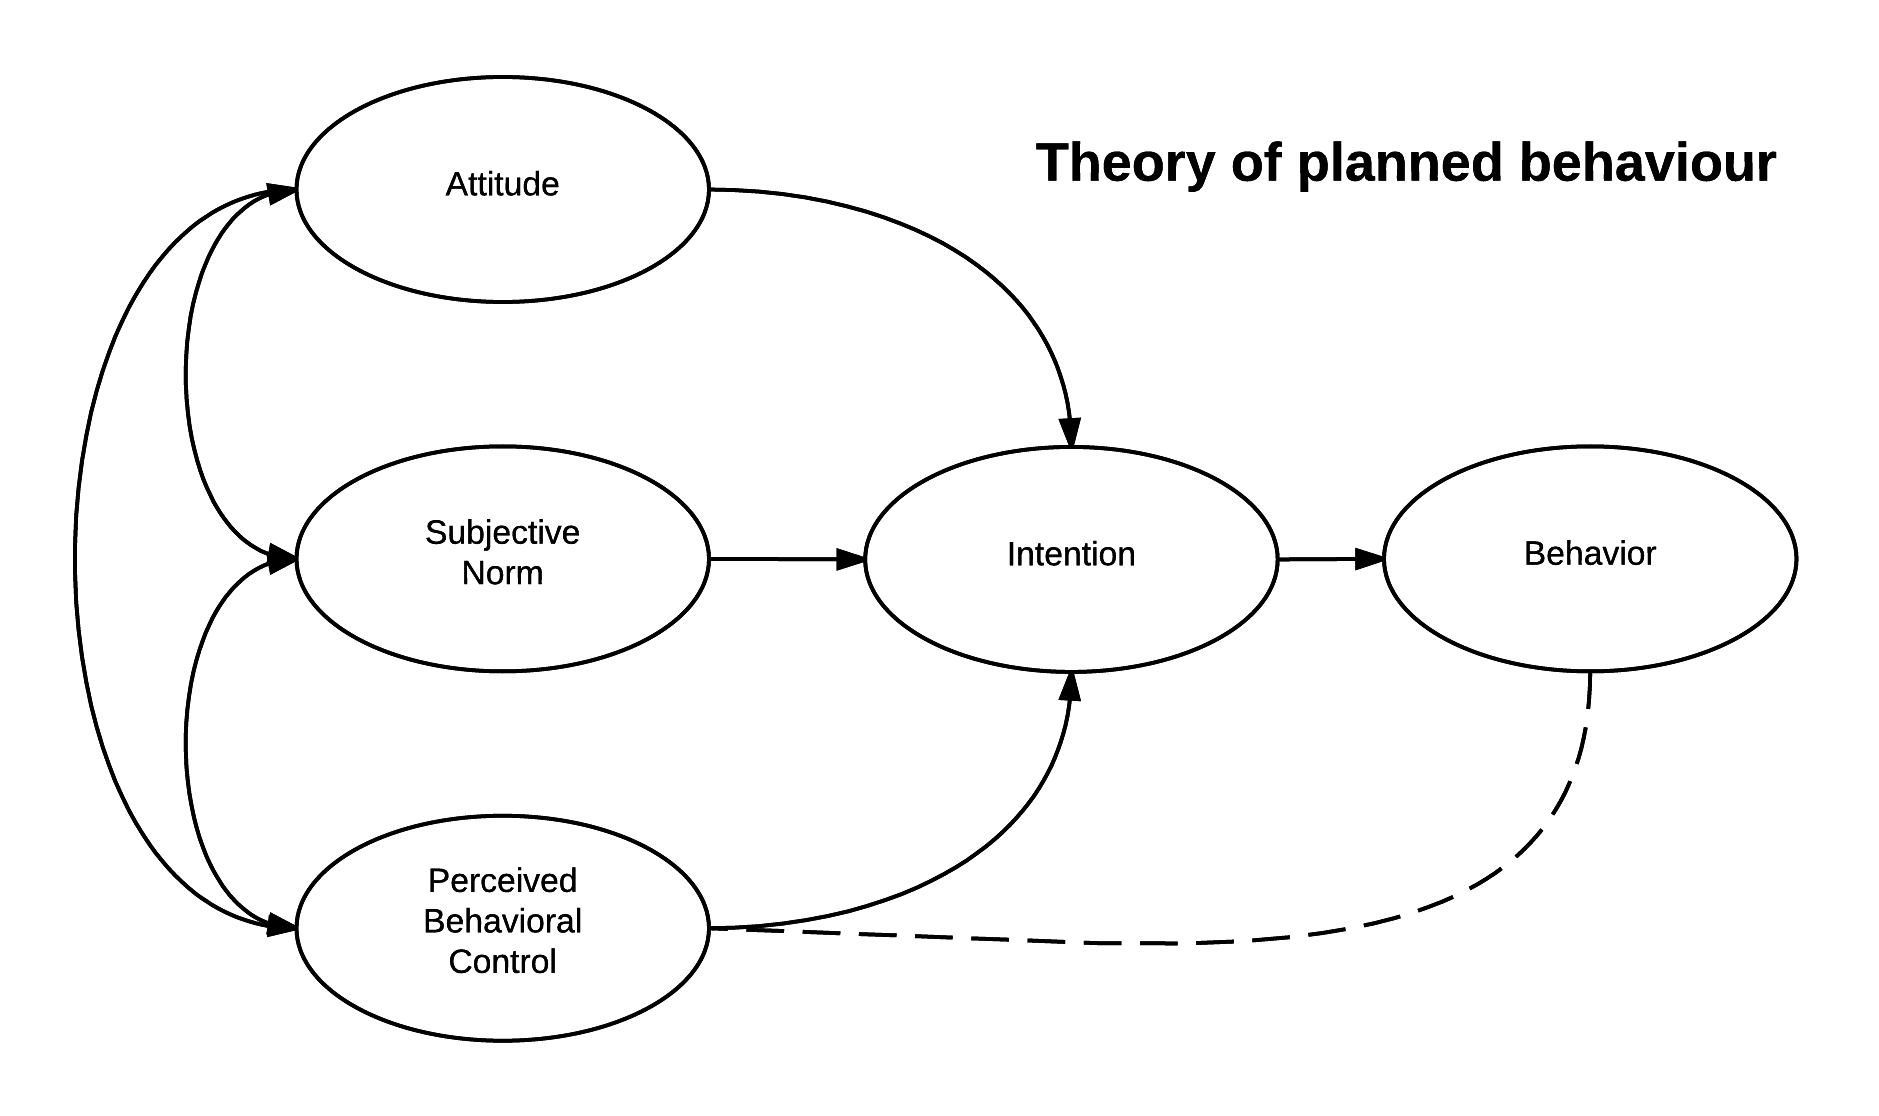
\includegraphics[width=0.8\textwidth]{Theory_of_planned_behavior_chart}}
    \caption{ساختار نظریه رفتار برنامه ریزی شده
      %\cite{kim2016integrated}
    }
    \label{fig:Theory_of_planned_behavior_chart}
  \end{figure}\\

  این نظریه در پژوهش‌های پیشین برای بررسی رفتار
  به اشتراک گذاری داده های خصوصی
  فرد در شبکه اجتماعی فیسبوک استفاده شده است
  \!\cite{vanderschyffInformationPrivacyBehavior2020}
  \!.
  مدلی که
  \!\gls{Theory of planned behavior}
  ارائه پیشنهاد می‌دهد، احتمال وقوع  رفتار‌های ارادی مخصوصا رفتار‌های ارادی مثبت به شدت تمایل فرد به
  انجام آن رفتار بستگی دارد.
  \!({\gls{Icek Ajzen}})
  عامل تعیین کننده برای انجام یک کار تمایلات او است.
\fi
%%%%%%%%%%%%%%%%%%%%

\ifSurveyfillingBehavior
  % بررسی اینکه آیا از نحوه پر کردن فرم ها می توان به کانفیدنس صداقت آزمودنی پی برد یا نه
  در صورتیکه گزینه‌های پرسشنامه اجباری باشند کیفیت داده‌های جمع‌آوری شده کاهش می یابد.
  \!\cite{sischkaImpactForcedAnswering2022}
\fi
% ^ %%%%%%%%%%%%%%%%%%%%%%%%%%%%%%%%%%%%%%%%%%%%%%%%%%%%%%%%%%%%%
% ^ %%%%%%%%%%%%%%%%%%%%%%%%%%%%%%%%%%%%%%%%%%%%%%%%%%%%%%%%%%%%%
% ^ %%%%%%%%%%%%%%%%%%%%%%%%%%%%%%%%%%%%%%%%%%%%%%%%%%%%%%%%%%%%%
\section{اهمیت}
%% توضیح بیشتر اضافه گردد بعدا
پژوهش انجام شده در سال ۲۰۲۰ نشان می دهد که در بازار داده های خصوصی آنلاین بازیگران زیادی به عنوان واسطه وجود دارند.
\!\cite{agogoInvisibleMarketOnline2021}
همچنین با گسترش هر روزه سیستم های اطلاعاتی که به
جمع‌آوری، ذخیره‌سازی، پردازش و به‌اشتراک‌گذاری داده‌های
خصوصی افراد می‌پردازند بررسی فرایندهای
تصمیم گیری و پارامتر‌های تاثیر گذار
بر این تصمیم‌گیری دارای اهمیت شده است
\!.
\!\cite{spiekermannValuesEthicsInformation2022}
از سوی دیگر نگرش افراد تصمیم گیرنده نسبت به ارزش اطلاعات خصوصی افراد می تواند نقش مهمی در رفتار آنها داشته باشد.
پژوهش‌هایی برای اندازه‌گیری ارزش داده‌های خصوصی انجام شده است
\!\cite{  fastValuePersonalData2021a,wesselsSellNotSell2019,tangHowChineseWeb2021}
\ifWillingnessToPay
  مقایسه میان رفتار افراد در پژوهش‌های اندازه‌گیری
  \textit{تمایل به پرداخت}
  \LTRfootnote{willingness to pay}
  نشان داده است که
  \textit{تمایل به پرداخت }
  با استفاده از روش‌های فرضی مانند
  \textit{ارزشيابی مشروط}
  \LTRfootnote{contingent valuation }
  میان ۱۷ تا ۶۳ درصد بالاتر
  از روشهای غیر فرضی مانند
  \textit{حراج تجربی}
  \LTRfootnote{experimental auction}
  است.
  حراج تجربی به عنوان یک روش
  \textit{سازگار با انگیزه}
  \LTRfootnote{incentive compatibility}
  شناسایی شده‌است
  \!\citep{martinez-carrascoComparingHypotheticalNonhypothetical2015}
  .
  یک فرایند،
  \textit{سازگار با انگیزه}
  است وقتی‌که همه شرکت‌کنندگان فقط  با درنظر گرفتن ترجیهات واقعی خود، بهترین خروجی را بدست می‌آورند
  \!\citep{nisanAlgorithmicGameTheory2007}
  \!.


\fi
% ^ %%%%%%%%%%%%%%%%%%%%%%%%%%%%%%%%%%%%%%%%%%%%%%%%%%%%%%%%%%%%%
% ^ %%%%%%%%%%%%%%%%%%%%%%%%%%%%%%%%%%%%%%%%%%%%%%%%%%%%%%%%%%%%%
% ^ %%%%%%%%%%%%%%%%%%%%%%%%%%%%%%%%%%%%%%%%%%%%%%%%%%%%%%%%%%%%%

\section{فرضیه پژوهشی}

% ^ %%%%%%%%%%%%%%%%%%%%%%%%%%%%%%%%%%%%%%%%%%%%%%%%%%%%%%%%%%%%%
% ^ %%%%%%%%%%%%%%%%%%%%%%%%%%%%%%%%%%%%%%%%%%%%%%%%%%%%%%%%%%%%%
% ^ %%%%%%%%%%%%%%%%%%%%%%%%%%%%%%%%%%%%%%%%%%%%%%%%%%%%%%%%%%%%%

% کلیه فایل‌های لازم برای حروف‌چینی با کلاس فوق، داخل پوشه‌ای به نام
% \lr{tehran-thesis}
% قرار داده شده است. توجه داشته باشید که برای استفاده از این کلاس باید فونت‌های
% \lr{IRLotusICEE}
% و
% \lr{IRTitr}
% را داشته باشید (که همراه با این کلاس هست و نیاز به نصب نیست).
% قلم‌های
% \lr{IRLotusICEE}
% مستخرج از قلم‌های استاندارد
% \lr{IRLotus}
% شورای عالی اطلاع‌رسانی%
% \footnote{
% قلم‌های استاندارد
% \lr{IRFonts}
% از شورای عالی اطلاع‌رسانی، منطبق بر آخرین نسخه استاندارد یونیکد، استاندارد ملی ۶۲۱۹ و استاندارد
% \lr{Adobe Glyph Naming}
% هستند.
% }
% هستند که توسط دکتر بابایی‌زاده اصلاحاتی روی آنها صورت پذیرفته است: تبدیل صفر توپر به صفر توخالی (جهت تمایز بیشتر با نقطه) و اضافه شدن
% \textit{\textbf{حالت توپر و ایرانیک توأم}}،
% که این موارد در قلم‌های شورای عالی اطلاع‌رسانی وجود ندارد.

% \subsection{این همه فایل؟!}
% \label{muchFiles}
% از آنجایی که یک پایان‌نامه یا رساله، یک نوشته بلند محسوب می‌شود، لذا اگر همه تنظیمات و مطالب پایان‌نامه را داخل یک فایل قرار بدهیم، باعث شلوغی و سردرگمی می‌شود. به همین خاطر، قسمت‌های مختلف پایان‌نامه یا رساله  داخل فایل‌های جداگانه قرار گرفته است. مثلاً تنظیمات پایه‌ای کلاس داخل فایل
% \lr{tehran-thesis.cls}، 
% قسمت مشخصات فارسی پایان‌نامه داخل 
% \lr{faTitle.tex}،
% مطالب فصل اول داخل 
% \lr{chapter1.tex}
% و تنظیمات قابل تغییر توسط کاربر داخل 
% \lr{commands.tex}،
% قرار داده شده است.
% \textbf{
% 	فایل اصلی این مجموعه، فایل
% 	\lr{main.tex}
% 	می‌باشد.
% }
% % یعنی بعد از تغییر فایل‌های دیگر، برای دیدن نتیجه تغییرات، باید این فایل را اجرا کرد. بقیه فایل‌ها به این فایل، کمک می‌کنند تا بتوانیم خروجی کار را ببینیم.
% اگر به فایل 
% \lr{main.tex}
% دقت کنید، متوجه می‌شوید که قسمت‌های مختلف پایان‌نامه، توسط دستورهایی مانند 
% \lr{input}
% و
% \lr{include}
% به فایل اصلی، یعنی 
% \lr{main.tex}
% معرفی شده‌اند.
% با توجه به ساختار محتوایی دستورالعمل، در فایل
% \lr{main.tex}
% فرض شده که پایان‌نامه یا رساله شما، از ۵ فصل و تعدادی پیوست تشکیل شده است. با اینحال، شما می‌توانید به راحتی فصل‌ها و پیوست‌ها را با صلاحدید اساتید راهنما، کم و زیاد کنید. این کار، بسیار ساده است. فرض کنید بخواهید یک فصل دیگر هم به پایان‌نامه اضافه کنید. برای این کار، کافی است یک فایل با نام دلخواه مثلاً 
% \lr{chapter6}
% و با پسوند 
% \lr{.tex}
% بسازید و آن را داخل پوشه 
% \lr{tehran-thesis}
% قرار دهید و سپس این فایل را با دستور 
% \verb!\include{chapter6}!
% داخل فایل
% \lr{main.tex}
%  فراخوانی کنید.

% \subsection{از کجا شروع کنم؟}
% قبل از هر چیز، باید یک توزیع تِک مناسب مانند تک‌لایو
% \lr{(TeXLive)}
% را روی سیستم خود نصب کنید. تک‌لایو  را می‌توانید از 
%  \href{http://www.tug.org/texlive}{سایت رسمی آن}%
% \LTRfootnote{\lr{\url{http://www.tug.org/texlive}}}
%  دانلود کنید یا مستقیماً از مخازن توزیع لینوکس خود بگیرید (مثلاً در اوبونتو با دستور
% \LRE{\verb!sudo apt install texlive-full!}).
% برای نصب تک‌لایو و اجرای اسناد زی‌پرشین می‌توانید از
% \href{http://parsilatex.com/site/shop/}{دی‌وی‌دی مجموعه پارسی‌لاتک}%
% \LTRfootnote{\lr{\url{http://parsilatex.com/site/shop/}}}
% و فایل راهنمای موجود در آن هم کمک بگیرید.

% برای تایپ و پردازش اسناد لاتک باید از یک ویرایشگر مناسب استفاده کنید. ویرایشگرهای
% \lr{TeXWroks},
% \lr{TeXstudio},
% \lr{Texmaker}
% و
% \lr{BiDiTeXmaker}
% بدین منظور تولید شده‌اند. می‌توان ویرایش‌گر 
%  \href{https://bitbucket.org/srazi/biditexmaker3}{\lr{BiDiTeXmaker}}%
%  \LTRfootnote{\lr{\url{https://bitbucket.org/srazi/biditexmaker3}}}
% را که بویژه برای کار با زی‌پرشین و مطالب دوجهته بهبود یافته است، بهینه‌ترین ویرایشگر لاتک برای کار با اسناد فارسی عنوان کرد.

% حال اگر نوشتن \پ اولین تجربه شما از کار با لاتک است، توصیه می‌شود که یک‌بار به صورت اجمالی، کتاب «%
% \href{http://www.tug.ctan.org/tex-archive/info/lshort/persian/lshort.pdf}{مقدمه‌ای نه چندان کوتاه بر
% \lr{\LaTeXe}}%
% \LTRfootnote{\lr{\url{http://www.tug.ctan.org/tex-archive/info/lshort/persian/lshort.pdf}\hfill}}»
% ترجمه دکتر مهدی امیدعلی را مطالعه کنید. این کتاب، کتاب بسیار کاملی است که خیلی از نیازهای شما در ارتباط با حروف‌چینی را برطرف می‌کند.
% اگر تک لایو کامل را داشته باشید، این کتاب را هم دارید. کافیست در خط فرمان دستور زیر را بزنید:
% \begin{latin}
% 	\texttt{texdoc lshort-persian}
% \end{latin}
% اگر عجله دارید، برخی دستورات پایه‌ای مورد نیاز در پیوست \ref{app:latexIntro} بیان شده‌اند.

% بعد از موارد گفته شده، فایل 
% \lr{main.tex}
% و
% \lr{faTitle.tex}
% را باز کنید و مشخصات پایان‌نامه خود مثل نام، نام خانوادگی، عنوان پایان‌نامه و ... را جایگزین مشخصات موجود در فایل
% \lr{faTitle.tex}
%  کنید. نیازی نیست نگران چینش این مشخصات در فایل پی‌دی‌اف خروجی باشید، زیرا کلاس 
% \lr{tehran-thesis}
% همه این کارها را بطور خودکار برای شما انجام می‌دهد. در ضمن، موقع تغییر دادن دستورهای داخل فایل
% \lr{faTitle.tex}
%  کاملاً دقت کنید؛ این دستورها، خیلی حساس هستند و ممکن است با یک تغییر کوچک، موقع اجرا، خطا بگیرید. برای دیدن خروجی کار، فایل 
% \lr{faTitle.tex}
%  را 
% \lr{Save}
% (نه 
% \lr{Save As})
% کنید و بعد به فایل 
% \lr{main.tex}
% برگشته و آن را اجرا کنید%
% \footnote{
% 	البته فایلهای این مجموعه به گونه‌ای هستند که در
% 	\lr{TeXWorks} یا
% 	\lr{TeXstudio}
% 	بدون بازگشت به فایل اصلی، می‌توانید سند خود را اجرا کنید.
% }.
%  حال اگر می‌خواهید مشخصات انگلیسی \پ را هم عوض کنید، فایل 
% \lr{enTitle.tex}
% را باز کنید و مشخصات داخلش را تغییر دهید.
% %\RTLfootnote{
% %برای نوشتن پروژه کارشناسی، نیازی به وارد کردن مشخصات انگلیسی پروژه نیست. بنابراین، این مشخصات بطور خودکار، نادیده گرفته می‌شود.
% %}
% در اینجا هم برای دیدن خروجی باید این فایل را ذخیره کرده، بعد به فایل 
% \lr{main.tex}
% برگشته و آن را اجرا کرد.

% برای راحتی بیشتر، کلاس 
% \lr{tehran-thesis.cls}
% طوری طراحی شده است که کافی است فقط  یک‌بار مشخصات \پ را (در فایل‌های
% \lr{faTitle.tex}
% و
% \lr{enTitle.tex})
% وارد کنید و هر جای دیگر که این مشخصات لازم باشند، به طور خودکار درج می‌شوند. با این حال، اگر مایل بودید، می‌توانید تنظیمات موجود را تغییر دهید؛ گرچه، در صورتیکه کاربر مبتدی هستید و یا با ساختار فایل‌های  
% \lr{cls}
%  آشنایی ندارید، بهتر است به فایل 
% \lr{tehran-thesis.cls}
% دست نزنید.

% نکته دیگری که باید به آن توجه کنید این است که در قالب آماده شده، سه گزینه به نام‌های
% \lr{bsc}،
% \lr{msc}
% و
% \lr{phd}
% برای نوشتن پروژه، پایان‌نامه و رساله، در نظر گرفته شده است. بنابراین اگر قصد تایپ پروژهٔ کارشناسی، پایان‌نامهٔ کارشناسی ارشد یا رسالهٔ دکتری را دارید، به ترتیب باید از گزینه‌های
% \lr{bsc}،
% \lr{msc}
% و
% \lr{phd}
% در فایل 
% \lr{main.tex}
% استفاده کنید. با انتخاب هر کدام از این گزینه‌ها، تنظیمات مربوط به آنها به طور خودکار، اعمال می‌شود.


% \subsection[مطالب پایان‌نامه را چطور بنویسم؟]
% {مطالب \پ را چطور بنویسم؟}
% \subsubsection{نوشتن فصل‌ها}
% همان‌طور که در بخش \ref{muchFiles} گفته شد برای جلوگیری از شلوغی، قسمت‌های مختلف \پ از جمله فصل‌ها، در فایل‌های جداگانه‌ای قرار داده شده‌اند. 
% مثلاً اگر می‌خواهید مطالب فصل ۱ را تایپ کنید، باید فایل‌های 
% \lr{main.tex}
% و
% \lr{chapter1.tex}
% را باز کرده و مطالب خود را جایگزین محتویات داخل 
% \lr{chapter1.tex}
% نمایید. دقت شود که در ابتدای برخی فایلها دستوراتی نوشته شده است و از شما خواسته شده که آن دستورات را حذف نکنید.

%توجه کنید که همان‌طور که قبلاً هم گفته شد، تنها فایل قابل اجرا، 
%\lr{main.tex}
%است. لذا برای دیدن حاصل (خروجی) فایل خود، باید  
%\lr{chapter1.tex}
%را ذخیره کرده و سپس فایل 
%\lr{main.tex}
%را اجرا کنید.

% نکته بسیار مهمی که در اینجا باید گفته شود این است که سیستم \lr{\TeX}، محتویات یک فایل تِک را به ترتیب پردازش می‌کند.  بنابراین، اگر مثلاً  دو فصل اول خود را نوشته و خروجی آنها را دیده‌اید و مشغول تایپ مطالب فصل ۳ هستید، بهتر است
% که دو دستور 
% \verb!% !TeX root=main.tex
% دستور زیر باعث شماره‌بندی صفحات فصول از ۱ می‌شود و باید در اولین فصل شما باشد. آن را حذف نکنید!
\pagenumbering{arabic} % 1, 2, ...

\chapter{مقدمه}
% دستور زیر باعث عدم‌نمایش شماره صفحه در اولین صفحه‌ی این فصل می‌شود.
%\thispagestyle{empty}
\ifDataveillance
  \textit{کریستین فوکس}
  \LTRfootnote{Christian Fuchs}
  جامعه شناس اتریشی،
  \textit{
    \gls{Social networking service}
  }
  \!({\lr{SNS}})
  در دنیای مدرن را به یک
  \textit{
    \gls{Panopticon}
  }
  تشبیه می کند   که در آن شرکت‌های بزرگی مانند
  \textit{
    \gls{Alphabet}
  }
  \!(
  شرکت مادر سرویس
  \textit{
    \gls{Google}
  }
  \!)
  و
  \textit{
    \gls{Meta}
  }
  \!(
  \!شرکت مادر و مالک برنامه‌های نرم‌افزاری مانند
  \textit{
    \gls{Instagram}
  }،
  \textit{
    \gls{Facebook}
  }
  و
  \textit{
    \gls{Whatsapp}
  }
  \!)
  به
  \textit{
    \gls{Dataveillance}
  }
  اعضا می‌پردازند
  \!\citep{romelePanopticismNotEnough2017a}.
  عبارت
  \textit{
    \gls{Panopticon}
  }
  را اولین بار
  \textit{
    \gls{Jeremy Bentham}
  }
  \!
  \citep{benthamPanopticonInspectionHouseContaining1791}
  برای توصیف ساختار‌های اجتماعی که مانند سیستم متمرکز نظارت عمل می‌کنند، از معماری وارد
  \textit{
    \gls{Social philosophy}
  }
  کرد.
\fi %Dataveillance
% * from old proposal and thesis fron khordad 1400 /media/d_drive/PJ/K/C/PJ-HDD-NiliLab/ssd2-laptop-backup-4mordad00/PJ/KN/Cog/proposal/tex/003
به نظر می‌رسد تصمیم‌گیرندگانی که در چنین سازمان‌هایی حضور دارند به حجم زیادی از اطلاعات
شخصی افراد دسترسی دارند. چنین افرادی، به علت وظیفه‌ای که در قبال سازمان
متبوع خود دارند، ملزم با حداکثر کردن سود بنگاه‌های اقتصادی هستند
که مالکیت این سازمان‌ها و سرویس‌های ارائه شده را، در اختیار
دارند.از طرف دیگر، همین تصمیمات می‌تواند باعث متضرر شدن
کاربرانی باشد که مالک اصلی اطلاعات جمع‌آوری شده می‌باشند. در چنین شرایطی، وقتی که
\textit{
  \glspl{Oversight institution}
}
با تغییرات سریع  در ساختارهای
\textit{
  \glspl{Information society}
}
ناهماهنگ هستند
\!\citep{cavoukianDiscussionPaperPrivacy2009,machovaDiscourseSurveillancePrivacy2021}،
بررسی ساز و کار موثر بر تصمیمات این افراد، اهمیت پیدا می‌کند.
اهمیت  این موضوع زمانی بیشتر می‌شود که کاربران
\textit{
  \gls{Social networking service}
}
تحت تاثیر
\textit{
  \glspl{Motivitions of}
}
متضاد قرار می‌گیرند و رفتاری را نشان می‌دهند که با عنوان
\textit{
  \gls{Privacy paradox}
}
شناخته می‌شود
\!citep{barthPrivacyParadoxInvestigating2017}.

این رفتار زمانی مشاهده می‌شود که کاربران شبکه‌های اجتماعی با وجود اهمیتی که برای حفظ
\textit{
  \gls{Information privacy}
}
بیان می‌کنند باز هم بی‌محابا نسبت به  منتشر کردن اطلاعات شخصی خود
در شبکه‌های اجتماعی اقدام می‌کنند.

این رفتار حتی پس از آگاه شدن از
پیامدهای سوءاستفاده از این اطلاعات نیز کاهش چشمگیری نداشته است
\!\citep{hermesWhoQuitsPrivacyInvasive2021,wirthLazinessExplanationPrivacy2022}.
به نظر می‌رسد که جلوگیری از پیامدهای  نامطلوب سوءاستفاده از اطلاعات خصوصی کاربران و نقض
\textit{
  \gls{Information privacy}
}
از طریق مداخلاتی که در سطح کاربران انجام شود، با توجه به گسترش و تنوع جمعیتی،
دشوار خواهد بود. با این وجود،
\textit{
  \gls{Information privacy}
}
که به توانایی افراد
برای کنترل اطلاعات مربوط به آنها اشاره دارد
\!{\cite{smithInformationPrivacyMeasuring1996}}
در سال‌های اخیر بیشتر مورد توجه کاربرانی قرار گرفته است
که داده‌های آنها توسط
\textit{
  \glspl{Social networking service}
}
جمع‌آوری، طبقه‌بندی و تحلیل می شود
\!{\cite{wallOrganizationalViolationsExternally2016}}
\!.
\textit{
  \gls{Information privacy}
}
با اشتراک‌گذاری اطلاعات شخصی توسط صاحب اطلاعات، در تضاد نیست.
\textit{
  \gls{Information privacy}
}
داشتن کنترل بر روی اطلاعات بعد از به  اشتراک‌گذاری، می‌باشد.
\!{\cite{acquistiEconomicsPrivacy2016}}.
به اشتراک گذاری اطلاعات شخصی از دید صاحبان اولیه اطلاعات،
به عنوان یک رفتار اجتماعی ناخوشایند و بالقوه ناهنجار، شناسایی شده است،
\!{\cite{norbergCopingInformationRequests2014}}،
اما به نظر می‌رسد چنین دیدگاهی با تعریفی که برای
\textit{
  \gls{Information privacy}
}
ارائه شد، در تضاد قرار می‌گیرد. اگر کاربران بتوانند بعد از
\textit{
  \gls{Disclosure}
}
اطلاعات خود، بر روی نحوه استفاده از آن کنترل داشته باشند،
\textit{
  \gls{Personal Information Sharing Behavior}
}
به تنهایی
اثرات مخربی در پی نخواهد داشت.  به علاوه
جمع‌آوری و پردازش اطلاعات می‌تواند نتایج سازنده‌ای، در سطح
اجتماعی و فردی داشته باشد
\!\citep{rockenbachProvidingPersonalInformation2020}.
افرادی که در
\textit{
  \glspl{Information society}
}
فاقد
\textit{
  \glspl{information record}
}
کافی در
\textit{
  \gls{Big data}
}
باشند، از جهات مختلف مورد
\textit{
  \gls{Discrimination}
}
قرار می‌گیرند
\!\citep{favarettoBigDataDiscrimination2019,lermanBigDataIts2013}.
با این دیدگاه، به اشتراک گذاری اطلاعات شخصی توسط صاحب اطلاعات، نه تنها
ناسازگارانه نیست، بلکه به یک رفتار
\textit{
  \gls{Prosocial}
}
تبدیل می‌شود. اطلاعات کاربران پس از
\textit{
  \gls{Disclosure}
}
در اختیار تصمیم‌گیرندگانی قرار می‌گیرد که در
\textit{
  \glspl{Social networking service}
}
مسئول جمع‌آوری، ذخیره‌سازی و پردازش اطلاعات هستند. به نظر می‌آید که حفظ
\textit{
  \gls{Information privacy}
}
و جلوگیری از اثرات مخرب اجتماعی و فردی سوءاستفاده از
اطلاعات شخصی انباشته شده، از طریق شناسایی عوامل موثر
بر تصمیم‌گیری این افراد و به اجرا در آوردن
مداخلات موثر در این سطح،نتایج بهتری در پی داشته باشد.

کاربران
\textit{
  \glspl{Social networking service}
}
پس از ارائه اطلاعات شخصی خود، خدماتی را از آن دریافت می‌کنند. این
تبادل میان کاربر و
\textit{
  \glspl{Social networking service}
}
مورد توافق طرفین است. شرایط حاکم بر این تبادل در توافق‌نامه‌ای
که در زمان عضویت به افراد ارائه می‌شود، مشخص شده است. به عنوان مثال
فرد در قبال اطلاعات شخصی خود از امکانات
\textit{
  \glspl{Social networking service}
}
برای برقراری ارتباط با دوستان خود استفاده می کند. او همچنین
با شروط دیگری که  برای عضویت لازم بوده است، موافقت کرده است. او
قبول کرده است که
\textit{
  \gls{Social networking service}
}
اطلاعات شخصی‌اش را در جهت ارائه تبلیغات هدفمند به کاربران، ذخیره کند
و مورد بازبینی و پردازش قرار دهد. اثرات مخرب این تبادل از زمانی شروع می شود که دریافت کننده اطلاعات، از
آن برای اهدافی به غیر از توافق اولیه استفاده کند و یا امکان این کار را برای یک شخص ثالث فراهم کند
\!{\cite{padyabExploringImpactsSecondary2018}}.

\textit{
  \gls{Secondary use of information}
}،
استفاده از اطلاعات شخصی برای اهدافی فراتر
از توافق اولیه، بعد از
\textit{
  \gls{Disclosure}
}
اطلاعات شخصی فرد، است. این عمل توسط موسسه جمع‌آوری کننده اطلاعات
و افراد تصمیم‌گیرنده در آن انجام می‌گیرد
\!{\cite{culnanHowDidThey1993}}.
پیامد‌های زیانبار تصمیمات بنگاه‌های اقتصادی و فن‌آوری بزرگی
مانند
\textit{
  \glspl{Meta}
}
برای استفاده ثانویه از اطلاعات شخصی جمع‌آوری شده، در پژوهش‌های مختلف بررسی شده اند
\!{\cite{padyabExploringImpactsSecondary2018}}.
این تصمیمات در سال‌های ۲۰۱۵ تا ۲۰۱۸، منجر به ناهنجاری‌های وسیع در سطح جوامع شدند
\!{\cite{redmanDataCredibilityProblem2013,dezwartSurveillanceBigData2014,spiekermannNetworksControlReport2016,schyffDuplicitouslMedia2020}}.
پیامدهای این ناهنجاری‌ها در نهایت افراد عضو جوامع را به طور غیر مستقیم
تحت تاثیر قرار می‌دهند. این افراد، متشکل از همان کاربرانی هستند که به طور جمعی، تامین کننده
داده‌های جمع‌آوری شده توسط
\textit{
  \glspl{Meta}
}
بوده‌اند.
\!{\cite{redmanDataCredibilityProblem2013,dezwartSurveillanceBigData2014,spiekermannNetworksControlReport2016,schyffDuplicitouslMedia2020}}.
با وجود آسیب‌پذیری افراد از داده‌های شخصی جمع‌آوری شده توسط شرکت‌ها
و شرکای تجاری آنها، تحقیقات نشان می‌دهد
که کاربران این جنبه تبادل اطلاعات خود را نادیده می‌گیرند
\!{\cite{raynes-goldieAliasesCreepingWall2010,brandtzaegTooManyFacebook2010,youngPrivacyProtectionStrategies2013}}،
هرچند با توجه به تاثیرات سازنده‌ای که برای رفتار اشتراک گذاری اطلاعات در بخش‌های
قبلی نام برده شده است، به نظر می‌رسد که می‌توان، تغییرات نامحسوس رفتار کاربران در
\textit{
  \gls{post–Cambridge Analytica scandal era}
}
\!{\citep{epsteinViewFramingDigital2021}}
را، پدیده مطلوبی توصیف کرد. با این وجود وقوع چنین پدیده‌هایی به 
\textit{
  \gls{Trust}
}
 در افراد جامعه آسیب می‌زند و در نهایت سبب کاهش منافع جمعیِ جمع‌آوری و پردازش اطلاعات، می‌گردد.


\gls{Cambridge Analytica scandal}
در سال ۲۰۱۶ باعث پی‌گیری‌ حقوقی شرکت 
\glspl{Meta} 
و مدیرعامل آن 
\textit{
  \gls{Mark Zuckerberg}
}
و محکومیت به پرداخت جریمه پنج میلیارد دلاری، شد
.\!{\citep{daviesFacebookPay5bn2019m,FacebookAgreesPay2019}}
واکنش مسؤولین فیسبوک نشان می‌دهد
که افراد تصمیم گیرنده در شرکت‌های جمع‌آوری کننده
اطلاعات نیز احتمالا از پیامدهایی که سیاست‌گذاری‌های آنها در استفاده ثانویه از اطلاعات شخصی کاربران
برای خود شرکت در پی دارد، ناآگاه هستند
\!{\cite{SuspendingCambridgeAnalytica2018,FacebookDataPrivacy2018}}
\!. با توجه به اینکه این افراد مسؤول حداکثر
کردن سود شرکت‌های خود هستند،
به نظر می‌رسد که چنین تصمیماتی فرض
\glspl{Rational}
بودن عامل‌های تصمیم‌گیرنده را در
\glspl{Rational choice theory}
به چالش می‌کشد. با در نظر گرفتن این مساله‌، ما در این پژوهش از از یک چارچوب نظری که فرض
\textit{
  \gls{Rational}
}
بودن تصمیمات را به چالش می‌کشند برای
\textit{
  \glspl{Articulation}
}
مفاهیم و رویکردهایمان استفاده کردیم.


تحقیقات زیادی برای بررسی رفتار کسانی که
اطلاعات خود را در اینترنت به اشتراک می‌گذارند انجام شده است
\!\!{\cite{kamleitnerInformationSharingPrivacy2019,kamleitnerYourDataMy2019}}.
همچنین رفتار افرادی که در مالکیت اطلاعت با فرد دیگر، شریک هستند بررسی شده است
\!\!{\cite{tawnieInterdependentPrivacy2017}}.
نتایج نشان می‌دهد که با وجود اینکه در همه جهان
\!،
\textit{
  \gls{Privacy}
}
اطلاعات شخصی افراد مساله مهمی برای کاربران آنلاین
است، بیشتر کاربران به ندرت برای محافظت از این داده، به خود زحمت می‌دهند و حتی در
بیشتر مواقع به طور داوطلبانه آن‌را پخش می‌کنند. تلاش زیادی انجام شده است تا این
دوگانگی میان
\textit{
  \gls{Privacy Attitude}
}
و رفتار، که معمولا با عنوان
\textit{
  \gls{Privacy paradox}
}
شناخته می‌شود، توضیح داده شود
\!\!{\cite{gerberExplainingPrivacyParadox2018}}.
به طور مشابه پژوهشی که در زمینه رفتار
\textit{
  \gls{Trust}
}
با به کار بردن
\textit{
  \gls{Theory of planned behavior}
}
در
\textit{
  \gls{Trust game}
}
انجام شده است،  وجود چنین تناقضی را در افراد
\textit{
  \gls{Trustor}
}
نیز نشان می‌دهد
\!\cite{gazdagNotWantTrust2019}.
به طور کلی، تا کنون  تحقیقات زیادی در حوزه
\textit{
  \gls{Information privacy}
}،
از
\textit{
  \gls{Trust game}
}
برای بررسی رفتار افراد در این تعامل
\textit{
  \gls{Interpersonal}
}،
استفاده کرده اند. با وجود اینکه تا به امروز رفتار کاربرانی که اطلاعات
\!(یا اطلاعات مشترک)
خود را به اشتراک می‌گذارند، مورد کنکاش قرار گرفته است، حیطه
رفتاری افرادی که دریافت کننده این  اطلاعات هستند به ندرت
مورد توجه قرار گرفته است
\!\cite{demmersYourDataAre2021}.

\subsection{کمبریج آنالیتیکا و استفاده ثانویه از اطلاعات}
در سال ۲۰۱۳ استاد دانشگاه کمبریج یک برنامه به نام 
«\lr{thisisyourdigitallife}»
ساخت. این برنامه در شبکه اجتماعی فیسبوک به کاربران 
آزمون‌های شخصیت‌شناسی ارائه می‌کرد. وقتی کاربر فیسبوک برنامه را بر روی حساب کاربری خود فعال و نصب
می‌کرد، برنامه جمع‌آوری اطلاعات شخصی او را آغاز می‌کرد. این اطلاعات شامل اطلاعات حساب کاربری و فعالیت‌های کاربر در فیسبوک
بود. فعالیت‌هایی مانند اینکه کاربر کدام محتوای فیسبوک را لایک کرده است. در حدود سیصد هزار نفر این 
برنامه را نصب کردند. اما اطلاعاتی که جمع‌آوری شد به این تعداد محدود نماند.  
این برنامه اطلاعاتی درباره دوستان کاربر که تنظیمات حریم خصوصی خود را درست  تنظیم نکرده بودند، را 
نیز جمع‌آوری کرد. در نتیجه برنامه توانست اطلاعات ۸۷ میلیون نفر را جمع‌آوری کند
\!\cite{kangFacebookSaysCambridge}.

سپس دکتر کوگان داده چمع‌آوری شده را به شرکت 
\textit{
  \gls{ Strategic Communication Laboratories (SCL)}
}
که مالک شرکت کمبریج آنالیتیکا است، انتقال داد. این شرکت یک موسسه مشاوره
سیاسی بود که از داده برای شناسایی ویژگی‌های شخصیتی و رفتار رای دهندگان
استفاده می‌کرد
\!\cite{rosenbergHowTrumpConsultants2018}. 
این شرکت از این داده برای کمک به به پویش محافظه‌کاران برای هدف
قرار دادن تبلیغات اینترنتی و پیام رسان‌ها استفاده کرد. این همان عملی 
بود که دکتر کوان شرایط و مقررات فیبوک را نقض کرد که انتقال یا 
فروش داده به هر شبکه تبلیغاتی ، دلال داده یا هر سرویس تبلیغاتی 
و درآمد‌زایی، ممنوع می‌کرد
\!\cite{granvilleFacebookCambridgeAnalytica2018}. 

وقتی در سال ۲۰۱۵ فیسبوک از این موضوع مطلع شد، برنامه دکتر کوگان 
را حذف  کرد و از کوگان و کمبریج آنالیتیکا درخواست کرد که
مدرکی ارائه دهند، که داده را پاک کرده‌اند. کوگان و کمبریج آنالیتیکا
به فیسبوک تاییده‌ای ارائه دادند که داده را حذف کرده‌اند. هرچند  کپی داده
خارج از کنترل فیسبوک باقی ماند.  وقتی الکساندر نیکس، مدیر عامل
کمبریج آنالیتیکا، به قانون‌گذاران گفت که شرکتش داده‌های فیسبوک را در
اختیار ندارد، یکی از کارمندان گفت که او اخیرا صدها گیگابایت داده را
بر روی سرورهای کمبریج آنالیتیکا دیده‌است و اطلاعات رمز نگاری نشده بودند.

در سال ۲۰۱۵، فیسبوک هیچ بیانیه عمومی‌ای درباره این رخداد منتشر نکرد. همچنین
کاربرانی که اطلاعات‌شان با کمبریج آنالیتیکا به اشتراک گذاشته شده 
بود. همچنین فیسبوک به کمیته تجارت فدرال، درباره این موضوع
چیزی نگفت. بر اساس آنچه که مارک زاکربرگ در کنفرانس دو روزه
 استماع‌اش در نهم و دهم آوریل ۲۰۱۸ گفت، به محض اینکه گواهی کمبریج آنالیتیکا
 مبنی بر حذف و تعهد عدم استفاده از داده را دریافت کردند، فیسبوک
 موضوع را خاتمه یافته تلقی کرد
 \!\cite{spanFacebookCEOMark}. 

 با منتشر شن این داستان در مارس ۲۰۱۸ در دو نشریه بین‌المللی، فیسبوک
 مطلع شد که داده تا آن روز پاک نشده بوده است. نتایج به بار آمده
 چنین حادثه‌ای بی سابقه بود. فیسبوک توسط چند نهاد قضایی در ایالت متحده، 
 جزیره انگلستان و اتحادیه اروپا مورد بازخواست قضایی قرار گرفت. یک پویش
 فیسبوک را حذف کنید راه افتاد و افت شدید قیمت سهام باعث شد تقریبا پنجاه میلیارد دلار
 سرمایه شرکت در عرض سه روز پس از فاش شدن اخبار، از بین رفت.




%   \glspl{phenomenon of dyadic completion}
%   نشان می دهد که گرایش های
%   \glspl{deontological}
%   و
%   \glspl{utilitarian}
%   نه تنها به طور همزمان فعال هستند
%   بلکه اغلب سازگار و تقویت کننده می‌باشند
%   \!{\cite{grayTwoMindsVs2012}}.
\subsection{چارچوب‌های نظری}
\textit{
  \gls{Rational choice theory}
}
\!{\cite{beckerEconomicApproachHuman1978}}،
این فرض را بنا می‌نهد که انسان‌ها بر اساس
تابعی از مجموع منفعت، با کسر مجموع هزینه‌های یک تصمیم
یا مبادله و برای حداکثر کردن فایده  شخصی دست به عمل می‌زنند.

این موضوع پایه‌ای برای طرح نظریه
\textit{
  \gls{Theory of reasoned action}
}
توسط
\textit{
  \gls{Icek Ajzen}
}
و
\textit{
  \gls{Martin Fishbein}
}
در در دهه ۸۰ میلادی شد. این نظریات پیشنهاد می‌کنند که بین
\textit{
  \gls{Atteutude}
}
و رفتار رابطه وجود دارد
\!{\cite{ajzenPredictionGoaldirectedBehavior1986}}.
فهم رفتار اختیاری افراد به وسیله
بررسی انگیزه‌هایی که باعث اجرای یک عمل می شود، هدف اصلی این نظریه بود. این نظریه
بیان می کند که قصد اجرای یک عمل پیش‌بینی‌کننده اصلی انجام یا عدم ایجاد رفتار  است. به
علاوه پارامتر هنجاری
(هنجارهای اجتماعی که عمل را احاطه کرده‌اند)
در اجرا شدن یا نشدن عمل نقش بازی می کند
\!{\citep{HealthBehaviorTheory2015,doswellTestingTheoryReasoned2011,ajzenAttitudesAttitudeBehaviorRelation2000}}
.
اما تحقیقاتی که در قالب چارچوب‌های
\textit{
  \gls{Behavioral economics}
}
انجام شد، این فرض را مورد تردید قرار داده اند
\!\cite{henrichEconomicManCrosscultural2005}.
برای رفع کاستی‌های
\textit{
  \gls{Theory of reasoned action}
}
آیزن در سال ۱۹۹۱ 
\!\citep{ajzenTheoryPlannedBehavior1991}
\textit{
  \gls{Theory of planned behavior}
}
را مطرح کرد. به بیان این تئوری سه پارامتر اصلی
\textit{
  \gls{Attitude}
}
\!،
\textit{\gls{Subjective norm}}
و
\textit{\gls{Perceived Behavioral control}}
\!،
\textit{\glspl{Behavioral intention}}
افراد را شکل می‌بخشند. پایه تفکر
\textit{
  \gls{Theory of planned behavior}
}
این است که
\textit{
  \gls{Personal Information Sharing Behavior}
}
از تعامل
\textit{\glspl{Psychological construct}}
\textit{
  \gls{Attitude}
}
\!،
\textit{\gls{Subjective norm}}،
\textit{\gls{Perceived Behavioral control}}
و
\textit{\glspl{Behavioral intention}}
نسبت به 
\textit{
  \gls{Personal Information Sharing}
}،
ایجاد می‌شود. 

در پژوهش‌های پیشین برای بررسی
\textit{
  \gls{Personal Information Sharing Behavior}
}
از
\textit{
  \gls{Theory of reasoned action}
}
\!\citep{malhotraInternetUsersInformation2004}،
و
\textit{
  \gls{Theory of planned behavior}
}
برای ایجاد ساختاری که روابط بین پارامترها را مدل می‌کند، استفاده شده است
\!\citep{dinevExtendedPrivacyCalculus2006b}.

در این پژوهش ما بررسی رفتار به اشتراک گذاری اطلاعات خصوصی دیگران در
\textit{
  \gls{Conceptual framework}
}
\textit{
  \gls{Theory of planned behavior}
}
پرداختیم.

برای سنجش رویکرد‍ افراد به
\textit{
  \gls{Personal information of Others}
}
یک پرسشنامه بر اساس دسته‌بندی‌های هفت‌گانه‌ای که در پژوهش پیشین با توجه به رویکرد صاحبان
اولیه اطلاعات خصوصی نسبت به خطر فاش شدن اطلاعات شخصی شان در حوزه‌های مختلف، ساخته شد.
این پرسشنامه برای هر دسته از سوالات دارای ۲ سوال است. برای اینکه بتوان باور 
آزمودنی‌ها، را هم بر اساس ارزش ذهنی خود
\!(نگرش به ارزش اطلاعات)
و هم بر اساس ارزش ذهنی دیگران
\!(هنجار ذهنی و باور هنجاری)
و همچنین برای اندازه‌گیری پایایی درونی،
سوالات به دو دسته تقسیم ‌می‌شود.
به هر آزمودنی، دسته اول اطلاعات خصوصی به همراه یک سوال برای سنجش باور هنجاری، و دسته دوم
اطلاعات به همراه سوال دیگر برای سنجش باور شخصی، ارائه شد. به طور تصادفی این دو دسته از 
سوالات برای هر آزمودنی جابجا شدند تا در نهایت پاسخ‌های نیمی از آزمونی‌ها به دسته اول سوالات از دید خود و نیمی 
دیگر از آزمودنی ها به دسته دوم سوالات از دید خود، جمع‌آوری شوند. به همین ترتیب پاسخ به سوالات دسته اول و دوم 
با توجه به باور هنجاری از دو دسته مستقل به تصادف انتخاب شدند، جمع‌آوری شد. تصادفی سازی در زمان وردو آزمودنی‌ها
به آزمایش با انتصاب افراد با احتمال ۵۰ درصد به دو گروه، انجام شد.
% * %%%%%%%%%%%%%%%%%%%%%%%%%%%%%%%%%%%%%%%%%% from old proposal and thesis from khordad 1400

\section{متغیر‌ها و پرسشنامه‌ها}

\ifPlennedBahaviorTheory
  \textit{\gls{Theory of planned behavior}}
  \!(TPB)
  % \LTRfootnote{Theory of planned behavior (TPB) }
  %  acronyms اضافه شود
  ، تعامل سه باور فردی شامل
  \textit{\gls{Atteutude}} ،
  \textit{\gls{Subjective norm}} و
  \textit{\gls{Perceived Behavioral control}}
  % \LTRfootnote{Perceived Behavioral control}
  را عامل رفتار می داند
  \!(شکل: \ref{fig:Theory_of_planned_behavior_chart})
  \!\cite{ajzenTheoryPlannedBehavior2020}.
  در این نظریه 
  \textit{\gls{Atteutude}}
 از دو نگرش احساسی و نگرش ابزاری تشکیل شده است.
  \textit{\gls{Subjective norm}}
  شامل  هنجارهای ذهنی و هنجار توصیفی است.
  \textit{\gls{Perceived Behavioral control}}،
  دو بخش کنترل رفتاری درک شده و خود کارآمدی درک شده را شامل می باشد
  در این نظریه عامل اصلی تعیین کننده
  رفتار، قصد رفتاری است و اجزای ساختاری این نظریه
  بر روی قصد تاثیر ویژه‌ای دارند
  \cite{mhmdpwrBrrsyTthyrTywry2022}
  \begin{figure}[ht]
    \centerline{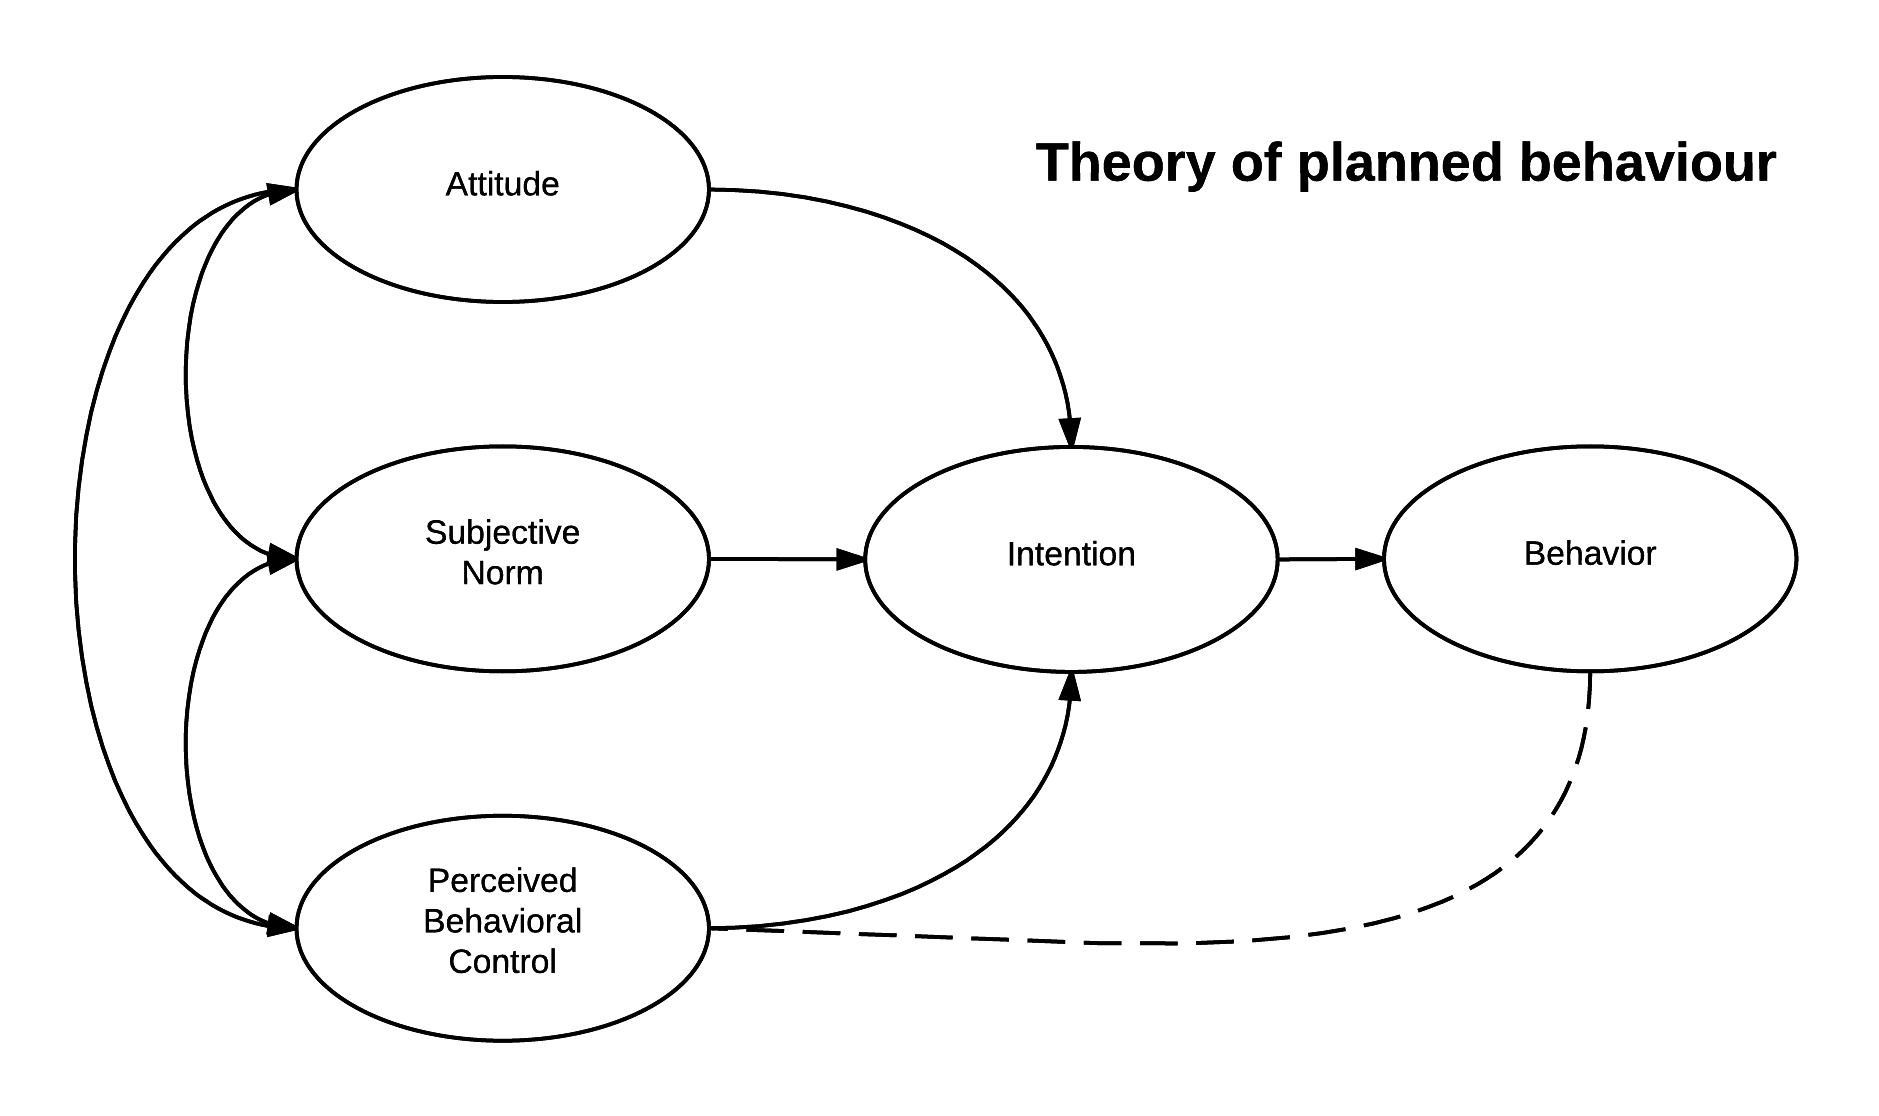
\includegraphics[width=0.8\textwidth]{Theory_of_planned_behavior_chart}}
    \caption{ساختار نظریه رفتار برنامه ریزی شده
      %\cite{kim2016integrated}
    }
    \label{fig:Theory_of_planned_behavior_chart}
  \end{figure}\\

  این نظریه در پژوهش‌های پیشین برای بررسی رفتار
  به اشتراک گذاری داده های خصوصی
  فرد در شبکه اجتماعی فیسبوک استفاده شده است
  \!\cite{vanderschyffInformationPrivacyBehavior2020}
  \!.
  مدلی که
  \!\gls{Theory of planned behavior}
  ارائه پیشنهاد می‌دهد، احتمال وقوع  رفتار‌های ارادی مخصوصا رفتار‌های ارادی مثبت به شدت تمایل فرد به
  انجام آن رفتار بستگی دارد.
  \!({\gls{Icek Ajzen}})
  عامل تعیین کننده برای انجام یک کار تمایلات او است.
\fi
%%%%%%%%%%%%%%%%%%%%

\ifSurveyfillingBehavior
  % بررسی اینکه آیا از نحوه پر کردن فرم ها می توان به کانفیدنس صداقت آزمودنی پی برد یا نه
  در صورتیکه گزینه‌های پرسشنامه اجباری باشند کیفیت داده‌های جمع‌آوری شده کاهش می یابد.
  \!\cite{sischkaImpactForcedAnswering2022}
\fi
% ^ %%%%%%%%%%%%%%%%%%%%%%%%%%%%%%%%%%%%%%%%%%%%%%%%%%%%%%%%%%%%%
% ^ %%%%%%%%%%%%%%%%%%%%%%%%%%%%%%%%%%%%%%%%%%%%%%%%%%%%%%%%%%%%%
% ^ %%%%%%%%%%%%%%%%%%%%%%%%%%%%%%%%%%%%%%%%%%%%%%%%%%%%%%%%%%%%%
\section{اهمیت}
%% توضیح بیشتر اضافه گردد بعدا
پژوهش انجام شده در سال ۲۰۲۰ نشان می دهد که در بازار داده های خصوصی آنلاین بازیگران زیادی به عنوان واسطه وجود دارند.
\!\cite{agogoInvisibleMarketOnline2021}
همچنین با گسترش هر روزه سیستم های اطلاعاتی که به
جمع‌آوری، ذخیره‌سازی، پردازش و به‌اشتراک‌گذاری داده‌های
خصوصی افراد می‌پردازند بررسی فرایندهای
تصمیم گیری و پارامتر‌های تاثیر گذار
بر این تصمیم‌گیری دارای اهمیت شده است
\!.
\!\cite{spiekermannValuesEthicsInformation2022}
از سوی دیگر نگرش افراد تصمیم گیرنده نسبت به ارزش اطلاعات خصوصی افراد می تواند نقش مهمی در رفتار آنها داشته باشد.
پژوهش‌هایی برای اندازه‌گیری ارزش داده‌های خصوصی انجام شده است
\!\cite{  fastValuePersonalData2021a,wesselsSellNotSell2019,tangHowChineseWeb2021}
\ifWillingnessToPay
  مقایسه میان رفتار افراد در پژوهش‌های اندازه‌گیری
  \textit{تمایل به پرداخت}
  \LTRfootnote{willingness to pay}
  نشان داده است که
  \textit{تمایل به پرداخت }
  با استفاده از روش‌های فرضی مانند
  \textit{ارزشيابی مشروط}
  \LTRfootnote{contingent valuation }
  میان ۱۷ تا ۶۳ درصد بالاتر
  از روشهای غیر فرضی مانند
  \textit{حراج تجربی}
  \LTRfootnote{experimental auction}
  است.
  حراج تجربی به عنوان یک روش
  \textit{سازگار با انگیزه}
  \LTRfootnote{incentive compatibility}
  شناسایی شده‌است
  \!\citep{martinez-carrascoComparingHypotheticalNonhypothetical2015}
  .
  یک فرایند،
  \textit{سازگار با انگیزه}
  است وقتی‌که همه شرکت‌کنندگان فقط  با درنظر گرفتن ترجیهات واقعی خود، بهترین خروجی را بدست می‌آورند
  \!\citep{nisanAlgorithmicGameTheory2007}
  \!.


\fi
% ^ %%%%%%%%%%%%%%%%%%%%%%%%%%%%%%%%%%%%%%%%%%%%%%%%%%%%%%%%%%%%%
% ^ %%%%%%%%%%%%%%%%%%%%%%%%%%%%%%%%%%%%%%%%%%%%%%%%%%%%%%%%%%%%%
% ^ %%%%%%%%%%%%%%%%%%%%%%%%%%%%%%%%%%%%%%%%%%%%%%%%%%%%%%%%%%%%%

\section{فرضیه پژوهشی}

% ^ %%%%%%%%%%%%%%%%%%%%%%%%%%%%%%%%%%%%%%%%%%%%%%%%%%%%%%%%%%%%%
% ^ %%%%%%%%%%%%%%%%%%%%%%%%%%%%%%%%%%%%%%%%%%%%%%%%%%%%%%%%%%%%%
% ^ %%%%%%%%%%%%%%%%%%%%%%%%%%%%%%%%%%%%%%%%%%%%%%%%%%%%%%%%%%%%%

% کلیه فایل‌های لازم برای حروف‌چینی با کلاس فوق، داخل پوشه‌ای به نام
% \lr{tehran-thesis}
% قرار داده شده است. توجه داشته باشید که برای استفاده از این کلاس باید فونت‌های
% \lr{IRLotusICEE}
% و
% \lr{IRTitr}
% را داشته باشید (که همراه با این کلاس هست و نیاز به نصب نیست).
% قلم‌های
% \lr{IRLotusICEE}
% مستخرج از قلم‌های استاندارد
% \lr{IRLotus}
% شورای عالی اطلاع‌رسانی%
% \footnote{
% قلم‌های استاندارد
% \lr{IRFonts}
% از شورای عالی اطلاع‌رسانی، منطبق بر آخرین نسخه استاندارد یونیکد، استاندارد ملی ۶۲۱۹ و استاندارد
% \lr{Adobe Glyph Naming}
% هستند.
% }
% هستند که توسط دکتر بابایی‌زاده اصلاحاتی روی آنها صورت پذیرفته است: تبدیل صفر توپر به صفر توخالی (جهت تمایز بیشتر با نقطه) و اضافه شدن
% \textit{\textbf{حالت توپر و ایرانیک توأم}}،
% که این موارد در قلم‌های شورای عالی اطلاع‌رسانی وجود ندارد.

% \subsection{این همه فایل؟!}
% \label{muchFiles}
% از آنجایی که یک پایان‌نامه یا رساله، یک نوشته بلند محسوب می‌شود، لذا اگر همه تنظیمات و مطالب پایان‌نامه را داخل یک فایل قرار بدهیم، باعث شلوغی و سردرگمی می‌شود. به همین خاطر، قسمت‌های مختلف پایان‌نامه یا رساله  داخل فایل‌های جداگانه قرار گرفته است. مثلاً تنظیمات پایه‌ای کلاس داخل فایل
% \lr{tehran-thesis.cls}، 
% قسمت مشخصات فارسی پایان‌نامه داخل 
% \lr{faTitle.tex}،
% مطالب فصل اول داخل 
% \lr{chapter1.tex}
% و تنظیمات قابل تغییر توسط کاربر داخل 
% \lr{commands.tex}،
% قرار داده شده است.
% \textbf{
% 	فایل اصلی این مجموعه، فایل
% 	\lr{main.tex}
% 	می‌باشد.
% }
% % یعنی بعد از تغییر فایل‌های دیگر، برای دیدن نتیجه تغییرات، باید این فایل را اجرا کرد. بقیه فایل‌ها به این فایل، کمک می‌کنند تا بتوانیم خروجی کار را ببینیم.
% اگر به فایل 
% \lr{main.tex}
% دقت کنید، متوجه می‌شوید که قسمت‌های مختلف پایان‌نامه، توسط دستورهایی مانند 
% \lr{input}
% و
% \lr{include}
% به فایل اصلی، یعنی 
% \lr{main.tex}
% معرفی شده‌اند.
% با توجه به ساختار محتوایی دستورالعمل، در فایل
% \lr{main.tex}
% فرض شده که پایان‌نامه یا رساله شما، از ۵ فصل و تعدادی پیوست تشکیل شده است. با اینحال، شما می‌توانید به راحتی فصل‌ها و پیوست‌ها را با صلاحدید اساتید راهنما، کم و زیاد کنید. این کار، بسیار ساده است. فرض کنید بخواهید یک فصل دیگر هم به پایان‌نامه اضافه کنید. برای این کار، کافی است یک فایل با نام دلخواه مثلاً 
% \lr{chapter6}
% و با پسوند 
% \lr{.tex}
% بسازید و آن را داخل پوشه 
% \lr{tehran-thesis}
% قرار دهید و سپس این فایل را با دستور 
% \verb!\include{chapter6}!
% داخل فایل
% \lr{main.tex}
%  فراخوانی کنید.

% \subsection{از کجا شروع کنم؟}
% قبل از هر چیز، باید یک توزیع تِک مناسب مانند تک‌لایو
% \lr{(TeXLive)}
% را روی سیستم خود نصب کنید. تک‌لایو  را می‌توانید از 
%  \href{http://www.tug.org/texlive}{سایت رسمی آن}%
% \LTRfootnote{\lr{\url{http://www.tug.org/texlive}}}
%  دانلود کنید یا مستقیماً از مخازن توزیع لینوکس خود بگیرید (مثلاً در اوبونتو با دستور
% \LRE{\verb!sudo apt install texlive-full!}).
% برای نصب تک‌لایو و اجرای اسناد زی‌پرشین می‌توانید از
% \href{http://parsilatex.com/site/shop/}{دی‌وی‌دی مجموعه پارسی‌لاتک}%
% \LTRfootnote{\lr{\url{http://parsilatex.com/site/shop/}}}
% و فایل راهنمای موجود در آن هم کمک بگیرید.

% برای تایپ و پردازش اسناد لاتک باید از یک ویرایشگر مناسب استفاده کنید. ویرایشگرهای
% \lr{TeXWroks},
% \lr{TeXstudio},
% \lr{Texmaker}
% و
% \lr{BiDiTeXmaker}
% بدین منظور تولید شده‌اند. می‌توان ویرایش‌گر 
%  \href{https://bitbucket.org/srazi/biditexmaker3}{\lr{BiDiTeXmaker}}%
%  \LTRfootnote{\lr{\url{https://bitbucket.org/srazi/biditexmaker3}}}
% را که بویژه برای کار با زی‌پرشین و مطالب دوجهته بهبود یافته است، بهینه‌ترین ویرایشگر لاتک برای کار با اسناد فارسی عنوان کرد.

% حال اگر نوشتن \پ اولین تجربه شما از کار با لاتک است، توصیه می‌شود که یک‌بار به صورت اجمالی، کتاب «%
% \href{http://www.tug.ctan.org/tex-archive/info/lshort/persian/lshort.pdf}{مقدمه‌ای نه چندان کوتاه بر
% \lr{\LaTeXe}}%
% \LTRfootnote{\lr{\url{http://www.tug.ctan.org/tex-archive/info/lshort/persian/lshort.pdf}\hfill}}»
% ترجمه دکتر مهدی امیدعلی را مطالعه کنید. این کتاب، کتاب بسیار کاملی است که خیلی از نیازهای شما در ارتباط با حروف‌چینی را برطرف می‌کند.
% اگر تک لایو کامل را داشته باشید، این کتاب را هم دارید. کافیست در خط فرمان دستور زیر را بزنید:
% \begin{latin}
% 	\texttt{texdoc lshort-persian}
% \end{latin}
% اگر عجله دارید، برخی دستورات پایه‌ای مورد نیاز در پیوست \ref{app:latexIntro} بیان شده‌اند.

% بعد از موارد گفته شده، فایل 
% \lr{main.tex}
% و
% \lr{faTitle.tex}
% را باز کنید و مشخصات پایان‌نامه خود مثل نام، نام خانوادگی، عنوان پایان‌نامه و ... را جایگزین مشخصات موجود در فایل
% \lr{faTitle.tex}
%  کنید. نیازی نیست نگران چینش این مشخصات در فایل پی‌دی‌اف خروجی باشید، زیرا کلاس 
% \lr{tehran-thesis}
% همه این کارها را بطور خودکار برای شما انجام می‌دهد. در ضمن، موقع تغییر دادن دستورهای داخل فایل
% \lr{faTitle.tex}
%  کاملاً دقت کنید؛ این دستورها، خیلی حساس هستند و ممکن است با یک تغییر کوچک، موقع اجرا، خطا بگیرید. برای دیدن خروجی کار، فایل 
% \lr{faTitle.tex}
%  را 
% \lr{Save}
% (نه 
% \lr{Save As})
% کنید و بعد به فایل 
% \lr{main.tex}
% برگشته و آن را اجرا کنید%
% \footnote{
% 	البته فایلهای این مجموعه به گونه‌ای هستند که در
% 	\lr{TeXWorks} یا
% 	\lr{TeXstudio}
% 	بدون بازگشت به فایل اصلی، می‌توانید سند خود را اجرا کنید.
% }.
%  حال اگر می‌خواهید مشخصات انگلیسی \پ را هم عوض کنید، فایل 
% \lr{enTitle.tex}
% را باز کنید و مشخصات داخلش را تغییر دهید.
% %\RTLfootnote{
% %برای نوشتن پروژه کارشناسی، نیازی به وارد کردن مشخصات انگلیسی پروژه نیست. بنابراین، این مشخصات بطور خودکار، نادیده گرفته می‌شود.
% %}
% در اینجا هم برای دیدن خروجی باید این فایل را ذخیره کرده، بعد به فایل 
% \lr{main.tex}
% برگشته و آن را اجرا کرد.

% برای راحتی بیشتر، کلاس 
% \lr{tehran-thesis.cls}
% طوری طراحی شده است که کافی است فقط  یک‌بار مشخصات \پ را (در فایل‌های
% \lr{faTitle.tex}
% و
% \lr{enTitle.tex})
% وارد کنید و هر جای دیگر که این مشخصات لازم باشند، به طور خودکار درج می‌شوند. با این حال، اگر مایل بودید، می‌توانید تنظیمات موجود را تغییر دهید؛ گرچه، در صورتیکه کاربر مبتدی هستید و یا با ساختار فایل‌های  
% \lr{cls}
%  آشنایی ندارید، بهتر است به فایل 
% \lr{tehran-thesis.cls}
% دست نزنید.

% نکته دیگری که باید به آن توجه کنید این است که در قالب آماده شده، سه گزینه به نام‌های
% \lr{bsc}،
% \lr{msc}
% و
% \lr{phd}
% برای نوشتن پروژه، پایان‌نامه و رساله، در نظر گرفته شده است. بنابراین اگر قصد تایپ پروژهٔ کارشناسی، پایان‌نامهٔ کارشناسی ارشد یا رسالهٔ دکتری را دارید، به ترتیب باید از گزینه‌های
% \lr{bsc}،
% \lr{msc}
% و
% \lr{phd}
% در فایل 
% \lr{main.tex}
% استفاده کنید. با انتخاب هر کدام از این گزینه‌ها، تنظیمات مربوط به آنها به طور خودکار، اعمال می‌شود.


% \subsection[مطالب پایان‌نامه را چطور بنویسم؟]
% {مطالب \پ را چطور بنویسم؟}
% \subsubsection{نوشتن فصل‌ها}
% همان‌طور که در بخش \ref{muchFiles} گفته شد برای جلوگیری از شلوغی، قسمت‌های مختلف \پ از جمله فصل‌ها، در فایل‌های جداگانه‌ای قرار داده شده‌اند. 
% مثلاً اگر می‌خواهید مطالب فصل ۱ را تایپ کنید، باید فایل‌های 
% \lr{main.tex}
% و
% \lr{chapter1.tex}
% را باز کرده و مطالب خود را جایگزین محتویات داخل 
% \lr{chapter1.tex}
% نمایید. دقت شود که در ابتدای برخی فایلها دستوراتی نوشته شده است و از شما خواسته شده که آن دستورات را حذف نکنید.

%توجه کنید که همان‌طور که قبلاً هم گفته شد، تنها فایل قابل اجرا، 
%\lr{main.tex}
%است. لذا برای دیدن حاصل (خروجی) فایل خود، باید  
%\lr{chapter1.tex}
%را ذخیره کرده و سپس فایل 
%\lr{main.tex}
%را اجرا کنید.

% نکته بسیار مهمی که در اینجا باید گفته شود این است که سیستم \lr{\TeX}، محتویات یک فایل تِک را به ترتیب پردازش می‌کند.  بنابراین، اگر مثلاً  دو فصل اول خود را نوشته و خروجی آنها را دیده‌اید و مشغول تایپ مطالب فصل ۳ هستید، بهتر است
% که دو دستور 
% \verb!\include{chapter1}!
% و
% \verb!\include{chapter2}!
% را در فایل 
% \lr{main.tex}،
% غیرفعال%
% \footnote{
% برای غیرفعال کردن یک دستور، کافی است در ابتدای آن، علامت درصد انگلیسی (\%) بگذارید.
% }
%  کنید. در غیر این صورت، ابتدا مطالب دو فصل اول پردازش شده و سپس مطالب فصل ۳ پردازش می‌شود که این کار باعث طولانی شدن زمان پردازش می‌گردد. هر زمان که خروجی کل \پ را خواستید، تمام فصل‌ها را دوباره در
% \lr{main.tex}
% فعال نمائید.
% بدیهتاً لازم نیست فصل‌های \پ را به ترتیب تایپ کنید. مثلاً می‌توانید ابتدا مطالب فصل ۳ را تایپ نموده و سپس مطالب فصل ۱ را تایپ کنید. 
% \subsubsection{مراجع}
% برای وارد کردن مراجع \پ کافی است فایل 
% \lr{MyReferences.bib}
% را باز کرده و مراجع خود را به شکل اقلام نمونهٔ داخل آن، وارد کنید.  سپس از \lr{bibtex} برای تولید مراجع با قالب مناسب استفاده نمائید. برای توضیحات بیشتر بخش \ref{Sec:Ref} از پیوست \ref{app:latexIntro} و نیز پیوست \ref{app:refMan} را ببینید.

% \subsubsection{واژه‌نامه فارسی به انگلیسی و برعکس}
% برای وارد کردن معادل فارسی اصطلاحات لاتین در متن و تهیه فهرست واژه‌نامه از آنها، از بستهٔ
% \lr{glossaries}
% و نرم‌افزار
% \lr{xindy}
% استفاده می‌شود. بدین منظور کافی است اصطلاحات لاتین و ترجمهٔ آنها را در فایل
% \lr{words.tex}
% وارد کرده و هر جای متن که خواستید با دستورات
% \verb|gls{label}|
% یا \verb|glspl{label}|
% معادل فارسی مفرد یا جمع یک اصطلاح را بیاورید.

% مثلا در اینجا، واژهٔ
% «\gls{Action}»
% برای بار اول و دوباره
% «\gls{Action}»
% برای بار دوم در متن ظاهر شده است.
% جهت توضیحات بیشتر به پیوست
% \ref{app:refMan}
% مراجعه کنید.
% \subsubsection{نمایه}
% برای وارد کردن نمایه، باید از 
% \lr{xindy}
% استفاده کنید. 
%زیرا 
%\lr{MakeIndex}
%با حروف «گ»، «چ»، «پ»، «ژ» و «ک» مشکل دارد و ترتیب الفبایی این حروف را رعایت نمی‌کند. همچنین، فاصله بین هر گروه از کلمات در 
%\lr{MakeIndex}،
%به درستی رعایت نمی‌شود که باعث زشت شدن حروف‌چینی این قسمت می‌شود. 
% راهنمای چگونگی کار با 
% \lr{xindy} 
% را می‌توانید در ویکی پارسی‌لاتک و یا مثالهای موجود در دی‌وی‌دی «مجموعه پارسی‌لاتک»، پیدا کنید.

% \subsection{اگر سوالی داشتم، از کی بپرسم؟}
% برای پرسیدن سوال‌های خود موقع حروف‌چینی با زی‌پرشین، می‌توانید به
% \href{http://qa.parsilatex.com}{سایت پرسش و پاسخ پارسی‌لاتک}%
% \LTRfootnote{http://qa.parsilatex.com}
% یا
% \href{http://forum.parsilatex.com}{بایگانی تالارگفتگوی قدیمی پارسی‌لاتک}%
% \mypagestye{http://forum.parsilatex.com}
% مراجعه کنید. شما هم می‌توانید روزی به سوال‌های دیگران در اینترنت جواب دهید.
% بستهٔ زی‌پرشین و بسیاری از بسته‌های مرتبط با آن مانند
% \lr{bidi} و
% \lr{Persian-bib}،
% مجموعه پارسی‌لاتک، مثالهای مختلف موجود در آن، قالب پایان‌نامه دانشگاههای مختلف و سایت پارسی‌لاتک همه به صورت داوطلبانه توسط افراد گروه پارسی‌لاتک و گروه
% \lr{Persian TeX}
% و بدون هیچ کمک مالی انجام شده‌اند. کار اصلی نوشتن و توسعه زی‌پرشین توسط آقای وفا خلیقی انجام شده است که این کار بزرگ را به انجام رساندند.
% اگر مایل به کمک به گروه پارسی‌لاتک هستید به سایت این گروه مراجعه فرمایید:
% \begin{center}
% 	\url{http://www.parsilatex.com}
% \end{center}

% \section{محتویات فصل اول یک پایان‌نامه}
% فصل اول یک پایان‌نامه باید به مقدمه یا کلیات تحقیق بپردازد.
% هدف از فصل مقدمه%
% \LTRfootnote{Introduction}،
% شرح مختصر مسأله تحقیق، اهمیت و انگیزه محقق از پرداختن به آن موضوع، بهمراه اشاره‌ای كوتاه به روش و مراحل تحقیق است. مقدمه، اولين فصل از ساختار اصلی \پ بوده و زمینه اطلاعاتی لازم را برای خواننده فراهم می‌آورد. در طول مقدمه باید سعی شود موضوع تحقیق با زبانی روشن، ساده و بطور عمیق و هدفمند به خواننده معرفی شود. این فصل باید خواننده را مجذوب و اهميت موضوع تحقيق را آشکار سازد. در مقدمه باید با ارائهٔ سوابق، شواهد تحقيقی و اطلاعات موجود (با ذکر منبع) با روشی منظم، منطقی و هدف‌دار، خواننده را جهت داد و به سوی راه حل مورد نظر هدايت کرد. مقدمه مناسب‌ترين جا برای ارائهٔ اختصارات و بعضی توضيحات کلی است، توضيحاتی که شايد نتوان در مباحث ديگر آنها را شرح داد.

% مقدمه، یکی از ارکان اساسی و اصلی پایان نامه است که مهمترین قسمت‌های آن عبارتند از: 

% \subsection{عنوان تحقیق} 
% باید شناختی دقیق و روشن از حوزهٔ موضوع تحقیق را عرضه دارد و خالی از هرگونه ابهام و پیچیدگی باشد.

% \subsection{مسأله تحقیق}
% وظیفه اصلی مقدمه بیان این مطلب به خواننده است که چرا انجام تحقیق را به عهده گرفته‌اید. اگر دلیل شما برای انجام این کار پاسخگویی به سؤال مورد علاقه‌تان است، با مشکل زیادی روبه‌رو نخواهید بود. یکی از بهترین روش‌ها برای نوشتن مقدمهٔ یک پایان‌نامه، طرح پرسش یا پرسش‌هایی مهم و اساسی است که کار تحقیقاتی شما از آغاز تا پایان قصد پاسخ دادن به آن را دارد. گاهی می‌توانید ابتدا اهمیت موضوع را بیان و سپس پرسش خود را در آن موضوع مطرح کنید.

% \subsection{تاریخچه‌ای از موضوع تحقیق}
% به طور کلی تشریح روندهای تحقیقاتی در محدودهٔ مورد مطالعه، مستلزم ارجاع به کارهای دیگران است. بعضی از نویسندگان برای کارهای دیگران هیچ اعتباری قائل نمی‌شوند و در مقابل، بعضی دیگر از نویسندگان در توصیف کارهای دیگران، بسیار زیاده‌روی می‌کنند. اکثر مواقع، ارجاع به مقالات دو سال قبل از کارتان، بهتر از نوشتن سطرهای مرجع است. در این قسمت باید به طور مختصر به نظرات و تحقیقات مربوط به موضوع و یا مسائل و مشکلات حل نشده در این حوزه و همچنین توجه و علاقه جامعه به این موضوع، اشاره شود.

% \subsection{تعریف موضوع تحقیق}
% در این قسمت محقق، موضوع مورد علاقه و یا نیاز احساس شدهٔ خود را در حوزه تحقیق بیان می‌دارد و عوامل موجود در موقعیت را تعریف و تعیین می‌کند.

% \subsection{هدف یا هدف‌های کلی و آرمانی تحقیق}
% این قسمت باید با جملات مثبت و کلی طرح شود و از طولانی شدن مطالب پرهیز شود.

% \subsection{روش انجام تحقیق}
% در این قسمت، پژوهشگر روش کاری خود را بیان می‌دارد و شیوه‌های گوناگونی را که در گردآوری مطالب خود بکار برده، ذکر می‌کند. همچنین اگر روش آماری خاصی را در تهیه و تدوین اطلاعات به کار برده است، آن شیوه را نیز اینجا بیان می‌کند.

% \subsection{نوآوری، اهمیت و ارزش تحقیق}
% در این قسمت، در مورد نوآوری علمی و عملی تحقیق که محقق به آن دست خواهد یافت، بحث می‌شود. ممکن است لازم باشد تا برخی نمودارهای خلاصه در این بخش استفاده شوند. به عنوان مثال، نموداری از مقاله
% \cite{kim2016integrated}
% در شکل
% \ref{fig:sampleDiagram}
% آمده است.
% \begin{figure}[ht]
% 	\centerline{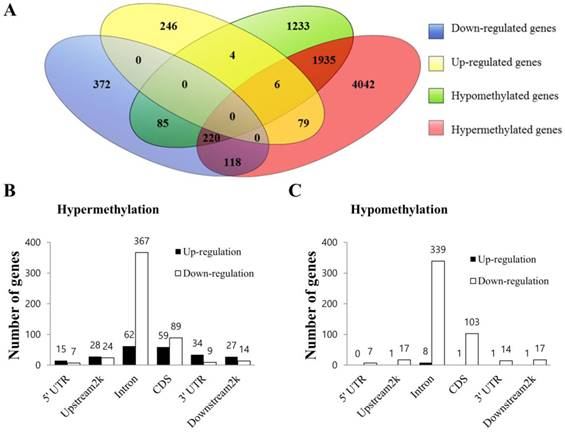
\includegraphics[width=0.8\textwidth]{journal-of-cancer_sample-result}}
% 	\caption{یک نمونه نمودار خلاصه برای نمایش نوآوری در نتایج
% 		%\cite{kim2016integrated}
% 	}
% 	\label{fig:sampleDiagram}
% \end{figure}\\
% طبیعتاً به صلاحدید نگارنده، شکل‌ها و نمودار‌ها می توانند در بخش های مختلف، خصوصا فصل
% \ref{chap:results}
% مورد استفاده قرار گیرند.

\subsection{تعریف واژه‌ها (اختیاری)}
% در این قسمت محقق باید واژه‌هایی را که ممکن است برای خواننده آشنا نباشد، تعریف کند.

\subsection{خلاصه فصل‌ها}
% در آخرین قسمتِ فصل اول پایان‌نامه، خلاصه‌ای اشاره‌وار از فصل‌های آتی آورده می‌شود تا خواننده بتواند تصویری واضح از دیگر قسمت‌های پایان‌نامه در ذهن خود ترسیم کند.

\section{جمع‌بندی}
% در این فصل به دو مقولهٔ نحوه استفاده از قالب \پ دانشگاه تهران و نیز ویژگی‌هایی که محتویات فصل اول پایان‌نامه (یعنی مقدمه) باید داشته باشند، پرداخته شد. با توجه به اینکه این راهنما نحوه استفاده از قالب را شرح داده، ملزومات محتوایی هر فصل پایان‌نامه را توضیح می‌دهد و در پیوست‌ها نیز نحوهٔ کار با لاتک را یادآوری خواهد کرد، بنابراین مطالعهٔ کامل آن مقداری وقت شما را خواهد گرفت؛ اما مطمئن باشید از اتلاف وقت شما در ادامه کارتان تا حد زیادی جلوگیری خواهد کرد. در نوشتن متن حاضر سعی شده است علاوه بر ایجاد یک قالب لاتک برای پایان‌نامه‌های دانشگاه تهران، نکات محتوایی هر فصل نیز گوشزد گردد. طبیعتاً برای نگارش پایان‌نامهٔ خود می‌بایست مطالب تمام فصل‌ها را خودتان بازنویسی کنید.

% در ادامهٔ این راهنما، تنها فصل‌هایی که یک پایان‌نامه باید داشته باشد و نیز خصوصیات یا ساختاری که محتویات هر فصل باید از آنها برخوردار باشد%
% \footnote{از روی فایل «تمپلیت نگارش و تدوین پایان‌نامه \cite{UTThesisGuide}»}،
% آورده می‌شوند. نهایتاً  در پیوست‌ها، مطالبی در باب یادآوری دستورات لاتک، نحوه نوشتن فرمول‌ها، تعاریف، قضایا، مثال‌ها، درج تصاویر، نمودارها، جداول و الگوریتم‌ها و نیز مدیریت مراجع، آمده است.

% همچنین توصیه اکید دارم که رفع خطاهایی که احتمالاً با آنها مواجه می‌شوید را به آخر موکول نفرمایید و به محض برخورد با خطا، آن را اشکال‌زدایی و برطرف نمائید.!
% و
% \verb!% !TeX root=main.tex
\chapter{مروری بر مطالعات انجام شده}
%\thispagestyle{empty} 
\section{مقدمه}
% هدف از اين فصل که با عنوان‌های  «مروری بر ادبیات موضوع%
% \LTRfootnote{Literature Review}»،
% «مروری بر منابع» و يا «مروری بر پیشینه تحقیق%
% \LTRfootnote{Background Research}»
% معرفی می‌شود، بررسی و طبقه‌بندی یافته‌های تحقیقات دیگر محققان در سطح دنیا و تعیین و شناسایی خلأهای تحقیقاتی است. آنچه را که تحقیق شما به دانش موجود اضافه می‌کند، مشخص کنید. طرح پیشینه تحقیق%
% \LTRfootnote{Background Information}
% یک مرور محققانه است و تا آنجا باید پیش برود که پیش‌زمینهٔ تاریخی مناسبی از تحقیق را بیان کند و جایگاه تحقیق فعلی را در میان آثار پیشین نشان دهد. برای این منظور منابع مرتبط با تحقیق را بررسی کنید، البته نه آنچنان گسترده که کل پیشینه تاریخی بحث را در برگیرد. برای نوشتن این بخش:
% \begin{itemize}
% 	\item
% 	دانستنی‌های موجود و پیش‌زمینهٔ تاریخی و وضعیت کنونی موضوع را چنان بیان کنید که خواننده بدون مراجعه به منابع پیشین، نتایج حاصل از مطالعات قبلی را درک و ارزیابی کند.
% 	\item
% 	نشان دهید که بر موضوع احاطه دارید. پرسش تحقیق را همراه بحث و جدل‌ها و مسائل مطرح شده بیان کنید و مهم‌ترین تحقیق‌های انجام شده در این زمینه را معرفی نمائید.
% 	\item
% 	ابتدا مطالب عمومی‌تر و سپس پژوهش‌های مشابه با کار خود را معرفی کرده و نشان دهید که تحقیق شما از چه جنبه‌ای با کار دیگران تشابه یا تفاوت دارد.
% 	\item
% 	اگر کارهای قبلی را خلاصه کرده‌اید، از پرداختن به جزئیات غیرضروری بپرهیزید. در عوض، بر یافته‌ها و مسائل روش‌شناختی مرتبط و نتایج اصلی تأکید کنید و اگر بررسی‌ها و منابع مروری عمومی دربارهٔ موضوع موجود است، خواننده را به آنها ارجاع دهید.
% \end{itemize}


% \section{مروری بر ادبیات موضوع}
% در این قسمت باید به کارهای مشابه دیگران در گذشته اشاره کرد و وزن بیشتر این قسمت بهتر است به مقالات ژورنالی سال‌های اخیر (۲ تا ۳ سال) تخصیص داده شود. به نتایج کارهای دیگران با ذکر دقیق مراجع باید اشاره شده و جایگاه و تفاوت تحقیق شما نیز با کارهای دیگران مشخص شود. استفاده از مقالات ژورنال‌های معتبر در دو یا سه سال اخیر، می‌تواند به اعتبار کار شما بیافزاید.

% \section{نتیجه‌گیری}
% ‌در نتیجه‌گیری آخر این فصل، با توجه به بررسی انجام شده بر روی مراجع تحقيق، بخش‌های قابل گسترش و تحقیق در آن حیطه و چشم‌اندازهای تحقیق مورد بررسی قرار می‌گیرند.	در برخی از تحقیقات، نتیجه نهایی فصل روش تحقیق، ارائهٔ یک چارچوب کار تحقیقی 
% \lr{(research framework)}
% است.
\ifExperimentalAuction
	تصمیم‌گیری های ما نمایشگر ارزشگذاری‌های ما هستند. اقتصاد‌دان‌ها
	\textit{ارزش اقتصادی}
	\LTRfootnote{economic value}
	این تصمیمات را با نرخی که فرد یک محصول یا دارایی را با  دیگری مبادله می کند ، بیان می‌کنند.
	این نرخ به وسیله
	\textit{تمایل به پرداخت }
	\LTRfootnote{willingness to pay}
	حداکثری فرد اندازه‌گیری می‌شود.
	\citep{luskExperimentalAuctionsMethods2007}
	\section{تعاریف، اصول و مبانی نظری}
	% این قسمت ارائهٔ خلاصه‌ای از دانش کلاسیک موضوع است. این بخش الزامی نیست و بستگی به نظر استاد راهنما دارد.

\fi

\ifTheEffectsOfDifferentPersonalData
	\textit{چاو، اوی و هربلاند}
	\LTRfootnote{Chua, H.N., J.S. Ooi, and A. Herbland}
	در سال ۲۰۲۱ اطلاعات شخصی را در ۶ دسته طبقه بندی کرده‌اند.
	\citep{chuaEffectsDifferentPersonal2021}
	جدول
	\eqref{tab:PICatAndChar}
	\begin{table}[ht]
		\caption{دسته‌ها و ویژگی‌های اطلاعت شخصی}
		\label{tab:PICatAndChar}
		\centering
		\onehalfspacing
		% \begin{tabular}{p{0.35\linewidth} | p{0.6\linewidth}}  
		\begin{tabularx}{\linewidth}{ r X }
			% \hline 
			دسته
			 &
			% درجه آزادی 
			% تبدیل مختصات &
			توضیح
			\\
			\hline
			سبک زندگی-رفتار(LB)
			 &
			% zotero://select/library/items/LCYS3GQ2
			% https://www.zotero.org/users/5038267/items/LCYS3GQ2
			%توضیح
			اطلاعت درباره ویژگی‌ها و سبک زندگی فرد که بر رابطه عاطفی یا
			اجتماعی، ترجیهات، عادات، باورها، یا دیدگاه‌های او اثر می‌گذارد.
			% مثال‌ها:
			% \lr{L1}:
			% باور
			% (
			% مانند باورهای مذهبی، باورهای فلسفی، افکار و غیره
			% )
			% % \hline 
			% \lr{L2}:
			% ترجیهات و علایق
			% (مانند نظرات، تمایلات، علایق، غذاهای مورد علاقه، رنگ‌ها، چیزهای
			% دوست‌داشتنی و دوست‌نداشتنی)
			% \lr{L3}:
			% رفتار
			% (مانند رفتار وبگردی، الگوی تماس‌ها، لینک‌های کلیک شده،
			% سبک زندگی رویکرد و غیره)
			% \lr{L4}:
			% خانواده/روابط عاطفی
			% (مانند ساختار خانواده، همشیرها، فرزندان، ازدواج‌ها، طلاق‌ها،
			% روابط عاطفی و غیره)
			\\
			اجتماعی-اقتصادی(SE)
			 &
			% ۳ & 
			% ویژگی دو &
			اطلاعاتی که سطح زندگی اقتصادی یا اجتماعی فرد را نشان می‌دهند یا
			می‌توان به وسیله این اطلاعات ویژگی‌های مزبور را استخراج کرد.
			% مثال‌ها;
			% \lr{S1}:
			% \lr{S1}:
			% \lr{S1}:
			\\
			ردیابی(T)
			 &
			اطلاعاتی که روش‌هایی را برای موقعیت‌یابی و تماس با فرد ایجاد می کند.
			% \hline 
			\\
			اقتصادی(F)
			 &
			اطلاعاتی که درآمد، حساب‌های مالی، اعتبار، توانایی خرید/خرج کردن، و
			دارایی‌های مورد تملک/اجاره شده/قرض گرفته شده را مشخص می کند.
			\\
			احراز هویت(A)
			 &
			اطلاعاتی که برای احراز هویت فرد به کار می‌روند.
			\\
			پزشکی-سلامت(MH)
			 &
			شرایط پزشکی  یا اطلاعات مرتبط با سلامت فرد.
			\\
		\end{tabularx}
	\end{table}
	% \begin{table}[ht]
	%     \caption{مدلهای تبدیل دیگر.}
	%     \label{tab:motionModelsCont}
	%     \centering
	%     \onehalfspacing
	%     \begin{tabularx}{\textwidth}{|r|c|l|X|}
	%         \hline نام مدل & درجه آزادی & تبدیل مختصات & توضیح \\ 
	%         \hline مشابهت & ۴ & $\begin{aligned} x'=sx\cos\theta - sy\sin\theta+t_x \\ y'=sx\sin\theta+sy\cos\theta+t_y  \end{aligned}$  & اقلیدسی+تغییرمقیاس \\ 		
	%         \hline آفین & ۶ & $\begin{aligned} x'=a_{11}x+a_{12}y+t_x \\ y'=a_{21}x+a_{22}y+t_y \end{aligned}$  & مشابهت+اریب‌شدگی \\
	%         \hline
	%     \end{tabularx}
	% \end{table}


	از سوی دیگر
\fi %TheEffectsOfDifferentPersonalData
\ifMultidimensionalNatureOfPrivacyRisksConceptualisationMeasurementAndImplicationsForDigitalServices
	در سال ۲۰۲۲
	\textit{
		\gls{Sabrina Karwatzki, Manuel Trenz and Daniel Veit}
	}
	 یک دسته‌بندی قاعده‌گرا
	\textit{
		\gls{Nomological}
	}
	و جامع از نگرانی‌های حریم خصوصی افراد بر اساس پژوهش های گذشته ارائه داده و اعتبار و روایی آن‌را مورد سنجش قرار‌داده‌اند
	\citep{karwatzkiMultidimensionalNaturePrivacy}
	\!.
	آنها ۷ دسته
	\textbf{
		خطر حریم خصوصی فیزیکی
		\lr{(PH)}
		\LTRfootnote{Physical privacy risk}
		،
		خطر حریم خصوصی اجتماعی
		\lr{(SO)}
		\LTRfootnote{Social privacy risk}
		،
		خطر حریم خصوصی مرتبط با منابع
		\lr{(RE)}
		\LTRfootnote{Resource-related privacy risk}
		،
		خطر حریم خصوصی روانشناختی
		\lr{(PS)}
		\LTRfootnote{Psychological privacy risk}
		،
		خطر حریم خصوصی مرتبط با تعقیب قانونی
		\lr{(PR)}
		\LTRfootnote{Prosecution-related privacy risk}
		،
		خطر حریم خصوصی مرتبط با شغل
		\lr{(CR)}
		\LTRfootnote{Career-related privacy risks}
		\textmd{و}
		خطر حریم خصوصی مرتبط با آزادی
		\lr{(FR)}
		\LTRfootnote{Freedom-related privacy risk}
	}
\fi %\ifMultidimensionalNatureOfPrivacyRisksConceptualisationMeasurementAndImplicationsForDigitalServices
را شناسایی کردند. ما
از این دسته‌بندی و توصیفاتی که در این پژوهش با دسته‌بندی‌های نامبرده مرتبط دانسته شده اند، استفاده کردیم.
!
% را در فایل 
% \lr{main.tex}،
% غیرفعال%
% \footnote{
% برای غیرفعال کردن یک دستور، کافی است در ابتدای آن، علامت درصد انگلیسی (\%) بگذارید.
% }
%  کنید. در غیر این صورت، ابتدا مطالب دو فصل اول پردازش شده و سپس مطالب فصل ۳ پردازش می‌شود که این کار باعث طولانی شدن زمان پردازش می‌گردد. هر زمان که خروجی کل \پ را خواستید، تمام فصل‌ها را دوباره در
% \lr{main.tex}
% فعال نمائید.
% بدیهتاً لازم نیست فصل‌های \پ را به ترتیب تایپ کنید. مثلاً می‌توانید ابتدا مطالب فصل ۳ را تایپ نموده و سپس مطالب فصل ۱ را تایپ کنید. 
% \subsubsection{مراجع}
% برای وارد کردن مراجع \پ کافی است فایل 
% \lr{MyReferences.bib}
% را باز کرده و مراجع خود را به شکل اقلام نمونهٔ داخل آن، وارد کنید.  سپس از \lr{bibtex} برای تولید مراجع با قالب مناسب استفاده نمائید. برای توضیحات بیشتر بخش \ref{Sec:Ref} از پیوست \ref{app:latexIntro} و نیز پیوست \ref{app:refMan} را ببینید.

% \subsubsection{واژه‌نامه فارسی به انگلیسی و برعکس}
% برای وارد کردن معادل فارسی اصطلاحات لاتین در متن و تهیه فهرست واژه‌نامه از آنها، از بستهٔ
% \lr{glossaries}
% و نرم‌افزار
% \lr{xindy}
% استفاده می‌شود. بدین منظور کافی است اصطلاحات لاتین و ترجمهٔ آنها را در فایل
% \lr{words.tex}
% وارد کرده و هر جای متن که خواستید با دستورات
% \verb|gls{label}|
% یا \verb|glspl{label}|
% معادل فارسی مفرد یا جمع یک اصطلاح را بیاورید.

% مثلا در اینجا، واژهٔ
% «\gls{Action}»
% برای بار اول و دوباره
% «\gls{Action}»
% برای بار دوم در متن ظاهر شده است.
% جهت توضیحات بیشتر به پیوست
% \ref{app:refMan}
% مراجعه کنید.
% \subsubsection{نمایه}
% برای وارد کردن نمایه، باید از 
% \lr{xindy}
% استفاده کنید. 
%زیرا 
%\lr{MakeIndex}
%با حروف «گ»، «چ»، «پ»، «ژ» و «ک» مشکل دارد و ترتیب الفبایی این حروف را رعایت نمی‌کند. همچنین، فاصله بین هر گروه از کلمات در 
%\lr{MakeIndex}،
%به درستی رعایت نمی‌شود که باعث زشت شدن حروف‌چینی این قسمت می‌شود. 
% راهنمای چگونگی کار با 
% \lr{xindy} 
% را می‌توانید در ویکی پارسی‌لاتک و یا مثالهای موجود در دی‌وی‌دی «مجموعه پارسی‌لاتک»، پیدا کنید.

% \subsection{اگر سوالی داشتم، از کی بپرسم؟}
% برای پرسیدن سوال‌های خود موقع حروف‌چینی با زی‌پرشین، می‌توانید به
% \href{http://qa.parsilatex.com}{سایت پرسش و پاسخ پارسی‌لاتک}%
% \LTRfootnote{http://qa.parsilatex.com}
% یا
% \href{http://forum.parsilatex.com}{بایگانی تالارگفتگوی قدیمی پارسی‌لاتک}%
% \mypagestye{http://forum.parsilatex.com}
% مراجعه کنید. شما هم می‌توانید روزی به سوال‌های دیگران در اینترنت جواب دهید.
% بستهٔ زی‌پرشین و بسیاری از بسته‌های مرتبط با آن مانند
% \lr{bidi} و
% \lr{Persian-bib}،
% مجموعه پارسی‌لاتک، مثالهای مختلف موجود در آن، قالب پایان‌نامه دانشگاههای مختلف و سایت پارسی‌لاتک همه به صورت داوطلبانه توسط افراد گروه پارسی‌لاتک و گروه
% \lr{Persian TeX}
% و بدون هیچ کمک مالی انجام شده‌اند. کار اصلی نوشتن و توسعه زی‌پرشین توسط آقای وفا خلیقی انجام شده است که این کار بزرگ را به انجام رساندند.
% اگر مایل به کمک به گروه پارسی‌لاتک هستید به سایت این گروه مراجعه فرمایید:
% \begin{center}
% 	\url{http://www.parsilatex.com}
% \end{center}

% \section{محتویات فصل اول یک پایان‌نامه}
% فصل اول یک پایان‌نامه باید به مقدمه یا کلیات تحقیق بپردازد.
% هدف از فصل مقدمه%
% \LTRfootnote{Introduction}،
% شرح مختصر مسأله تحقیق، اهمیت و انگیزه محقق از پرداختن به آن موضوع، بهمراه اشاره‌ای كوتاه به روش و مراحل تحقیق است. مقدمه، اولين فصل از ساختار اصلی \پ بوده و زمینه اطلاعاتی لازم را برای خواننده فراهم می‌آورد. در طول مقدمه باید سعی شود موضوع تحقیق با زبانی روشن، ساده و بطور عمیق و هدفمند به خواننده معرفی شود. این فصل باید خواننده را مجذوب و اهميت موضوع تحقيق را آشکار سازد. در مقدمه باید با ارائهٔ سوابق، شواهد تحقيقی و اطلاعات موجود (با ذکر منبع) با روشی منظم، منطقی و هدف‌دار، خواننده را جهت داد و به سوی راه حل مورد نظر هدايت کرد. مقدمه مناسب‌ترين جا برای ارائهٔ اختصارات و بعضی توضيحات کلی است، توضيحاتی که شايد نتوان در مباحث ديگر آنها را شرح داد.

% مقدمه، یکی از ارکان اساسی و اصلی پایان نامه است که مهمترین قسمت‌های آن عبارتند از: 

% \subsection{عنوان تحقیق} 
% باید شناختی دقیق و روشن از حوزهٔ موضوع تحقیق را عرضه دارد و خالی از هرگونه ابهام و پیچیدگی باشد.

% \subsection{مسأله تحقیق}
% وظیفه اصلی مقدمه بیان این مطلب به خواننده است که چرا انجام تحقیق را به عهده گرفته‌اید. اگر دلیل شما برای انجام این کار پاسخگویی به سؤال مورد علاقه‌تان است، با مشکل زیادی روبه‌رو نخواهید بود. یکی از بهترین روش‌ها برای نوشتن مقدمهٔ یک پایان‌نامه، طرح پرسش یا پرسش‌هایی مهم و اساسی است که کار تحقیقاتی شما از آغاز تا پایان قصد پاسخ دادن به آن را دارد. گاهی می‌توانید ابتدا اهمیت موضوع را بیان و سپس پرسش خود را در آن موضوع مطرح کنید.

% \subsection{تاریخچه‌ای از موضوع تحقیق}
% به طور کلی تشریح روندهای تحقیقاتی در محدودهٔ مورد مطالعه، مستلزم ارجاع به کارهای دیگران است. بعضی از نویسندگان برای کارهای دیگران هیچ اعتباری قائل نمی‌شوند و در مقابل، بعضی دیگر از نویسندگان در توصیف کارهای دیگران، بسیار زیاده‌روی می‌کنند. اکثر مواقع، ارجاع به مقالات دو سال قبل از کارتان، بهتر از نوشتن سطرهای مرجع است. در این قسمت باید به طور مختصر به نظرات و تحقیقات مربوط به موضوع و یا مسائل و مشکلات حل نشده در این حوزه و همچنین توجه و علاقه جامعه به این موضوع، اشاره شود.

% \subsection{تعریف موضوع تحقیق}
% در این قسمت محقق، موضوع مورد علاقه و یا نیاز احساس شدهٔ خود را در حوزه تحقیق بیان می‌دارد و عوامل موجود در موقعیت را تعریف و تعیین می‌کند.

% \subsection{هدف یا هدف‌های کلی و آرمانی تحقیق}
% این قسمت باید با جملات مثبت و کلی طرح شود و از طولانی شدن مطالب پرهیز شود.

% \subsection{روش انجام تحقیق}
% در این قسمت، پژوهشگر روش کاری خود را بیان می‌دارد و شیوه‌های گوناگونی را که در گردآوری مطالب خود بکار برده، ذکر می‌کند. همچنین اگر روش آماری خاصی را در تهیه و تدوین اطلاعات به کار برده است، آن شیوه را نیز اینجا بیان می‌کند.

% \subsection{نوآوری، اهمیت و ارزش تحقیق}
% در این قسمت، در مورد نوآوری علمی و عملی تحقیق که محقق به آن دست خواهد یافت، بحث می‌شود. ممکن است لازم باشد تا برخی نمودارهای خلاصه در این بخش استفاده شوند. به عنوان مثال، نموداری از مقاله
% \cite{kim2016integrated}
% در شکل
% \ref{fig:sampleDiagram}
% آمده است.
% \begin{figure}[ht]
% 	\centerline{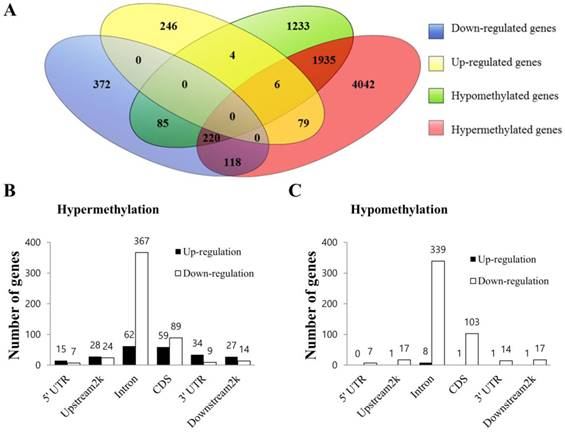
\includegraphics[width=0.8\textwidth]{journal-of-cancer_sample-result}}
% 	\caption{یک نمونه نمودار خلاصه برای نمایش نوآوری در نتایج
% 		%\cite{kim2016integrated}
% 	}
% 	\label{fig:sampleDiagram}
% \end{figure}\\
% طبیعتاً به صلاحدید نگارنده، شکل‌ها و نمودار‌ها می توانند در بخش های مختلف، خصوصا فصل
% \ref{chap:results}
% مورد استفاده قرار گیرند.

\subsection{تعریف واژه‌ها (اختیاری)}
% در این قسمت محقق باید واژه‌هایی را که ممکن است برای خواننده آشنا نباشد، تعریف کند.

\subsection{خلاصه فصل‌ها}
% در آخرین قسمتِ فصل اول پایان‌نامه، خلاصه‌ای اشاره‌وار از فصل‌های آتی آورده می‌شود تا خواننده بتواند تصویری واضح از دیگر قسمت‌های پایان‌نامه در ذهن خود ترسیم کند.

\section{جمع‌بندی}
% در این فصل به دو مقولهٔ نحوه استفاده از قالب \پ دانشگاه تهران و نیز ویژگی‌هایی که محتویات فصل اول پایان‌نامه (یعنی مقدمه) باید داشته باشند، پرداخته شد. با توجه به اینکه این راهنما نحوه استفاده از قالب را شرح داده، ملزومات محتوایی هر فصل پایان‌نامه را توضیح می‌دهد و در پیوست‌ها نیز نحوهٔ کار با لاتک را یادآوری خواهد کرد، بنابراین مطالعهٔ کامل آن مقداری وقت شما را خواهد گرفت؛ اما مطمئن باشید از اتلاف وقت شما در ادامه کارتان تا حد زیادی جلوگیری خواهد کرد. در نوشتن متن حاضر سعی شده است علاوه بر ایجاد یک قالب لاتک برای پایان‌نامه‌های دانشگاه تهران، نکات محتوایی هر فصل نیز گوشزد گردد. طبیعتاً برای نگارش پایان‌نامهٔ خود می‌بایست مطالب تمام فصل‌ها را خودتان بازنویسی کنید.

% در ادامهٔ این راهنما، تنها فصل‌هایی که یک پایان‌نامه باید داشته باشد و نیز خصوصیات یا ساختاری که محتویات هر فصل باید از آنها برخوردار باشد%
% \footnote{از روی فایل «تمپلیت نگارش و تدوین پایان‌نامه \cite{UTThesisGuide}»}،
% آورده می‌شوند. نهایتاً  در پیوست‌ها، مطالبی در باب یادآوری دستورات لاتک، نحوه نوشتن فرمول‌ها، تعاریف، قضایا، مثال‌ها، درج تصاویر، نمودارها، جداول و الگوریتم‌ها و نیز مدیریت مراجع، آمده است.

% همچنین توصیه اکید دارم که رفع خطاهایی که احتمالاً با آنها مواجه می‌شوید را به آخر موکول نفرمایید و به محض برخورد با خطا، آن را اشکال‌زدایی و برطرف نمائید.!
% و
% \verb!% !TeX root=main.tex
\chapter{مروری بر مطالعات انجام شده}
%\thispagestyle{empty} 
\section{مقدمه}
% هدف از اين فصل که با عنوان‌های  «مروری بر ادبیات موضوع%
% \LTRfootnote{Literature Review}»،
% «مروری بر منابع» و يا «مروری بر پیشینه تحقیق%
% \LTRfootnote{Background Research}»
% معرفی می‌شود، بررسی و طبقه‌بندی یافته‌های تحقیقات دیگر محققان در سطح دنیا و تعیین و شناسایی خلأهای تحقیقاتی است. آنچه را که تحقیق شما به دانش موجود اضافه می‌کند، مشخص کنید. طرح پیشینه تحقیق%
% \LTRfootnote{Background Information}
% یک مرور محققانه است و تا آنجا باید پیش برود که پیش‌زمینهٔ تاریخی مناسبی از تحقیق را بیان کند و جایگاه تحقیق فعلی را در میان آثار پیشین نشان دهد. برای این منظور منابع مرتبط با تحقیق را بررسی کنید، البته نه آنچنان گسترده که کل پیشینه تاریخی بحث را در برگیرد. برای نوشتن این بخش:
% \begin{itemize}
% 	\item
% 	دانستنی‌های موجود و پیش‌زمینهٔ تاریخی و وضعیت کنونی موضوع را چنان بیان کنید که خواننده بدون مراجعه به منابع پیشین، نتایج حاصل از مطالعات قبلی را درک و ارزیابی کند.
% 	\item
% 	نشان دهید که بر موضوع احاطه دارید. پرسش تحقیق را همراه بحث و جدل‌ها و مسائل مطرح شده بیان کنید و مهم‌ترین تحقیق‌های انجام شده در این زمینه را معرفی نمائید.
% 	\item
% 	ابتدا مطالب عمومی‌تر و سپس پژوهش‌های مشابه با کار خود را معرفی کرده و نشان دهید که تحقیق شما از چه جنبه‌ای با کار دیگران تشابه یا تفاوت دارد.
% 	\item
% 	اگر کارهای قبلی را خلاصه کرده‌اید، از پرداختن به جزئیات غیرضروری بپرهیزید. در عوض، بر یافته‌ها و مسائل روش‌شناختی مرتبط و نتایج اصلی تأکید کنید و اگر بررسی‌ها و منابع مروری عمومی دربارهٔ موضوع موجود است، خواننده را به آنها ارجاع دهید.
% \end{itemize}


% \section{مروری بر ادبیات موضوع}
% در این قسمت باید به کارهای مشابه دیگران در گذشته اشاره کرد و وزن بیشتر این قسمت بهتر است به مقالات ژورنالی سال‌های اخیر (۲ تا ۳ سال) تخصیص داده شود. به نتایج کارهای دیگران با ذکر دقیق مراجع باید اشاره شده و جایگاه و تفاوت تحقیق شما نیز با کارهای دیگران مشخص شود. استفاده از مقالات ژورنال‌های معتبر در دو یا سه سال اخیر، می‌تواند به اعتبار کار شما بیافزاید.

% \section{نتیجه‌گیری}
% ‌در نتیجه‌گیری آخر این فصل، با توجه به بررسی انجام شده بر روی مراجع تحقيق، بخش‌های قابل گسترش و تحقیق در آن حیطه و چشم‌اندازهای تحقیق مورد بررسی قرار می‌گیرند.	در برخی از تحقیقات، نتیجه نهایی فصل روش تحقیق، ارائهٔ یک چارچوب کار تحقیقی 
% \lr{(research framework)}
% است.
\ifExperimentalAuction
	تصمیم‌گیری های ما نمایشگر ارزشگذاری‌های ما هستند. اقتصاد‌دان‌ها
	\textit{ارزش اقتصادی}
	\LTRfootnote{economic value}
	این تصمیمات را با نرخی که فرد یک محصول یا دارایی را با  دیگری مبادله می کند ، بیان می‌کنند.
	این نرخ به وسیله
	\textit{تمایل به پرداخت }
	\LTRfootnote{willingness to pay}
	حداکثری فرد اندازه‌گیری می‌شود.
	\citep{luskExperimentalAuctionsMethods2007}
	\section{تعاریف، اصول و مبانی نظری}
	% این قسمت ارائهٔ خلاصه‌ای از دانش کلاسیک موضوع است. این بخش الزامی نیست و بستگی به نظر استاد راهنما دارد.

\fi

\ifTheEffectsOfDifferentPersonalData
	\textit{چاو، اوی و هربلاند}
	\LTRfootnote{Chua, H.N., J.S. Ooi, and A. Herbland}
	در سال ۲۰۲۱ اطلاعات شخصی را در ۶ دسته طبقه بندی کرده‌اند.
	\citep{chuaEffectsDifferentPersonal2021}
	جدول
	\eqref{tab:PICatAndChar}
	\begin{table}[ht]
		\caption{دسته‌ها و ویژگی‌های اطلاعت شخصی}
		\label{tab:PICatAndChar}
		\centering
		\onehalfspacing
		% \begin{tabular}{p{0.35\linewidth} | p{0.6\linewidth}}  
		\begin{tabularx}{\linewidth}{ r X }
			% \hline 
			دسته
			 &
			% درجه آزادی 
			% تبدیل مختصات &
			توضیح
			\\
			\hline
			سبک زندگی-رفتار(LB)
			 &
			% zotero://select/library/items/LCYS3GQ2
			% https://www.zotero.org/users/5038267/items/LCYS3GQ2
			%توضیح
			اطلاعت درباره ویژگی‌ها و سبک زندگی فرد که بر رابطه عاطفی یا
			اجتماعی، ترجیهات، عادات، باورها، یا دیدگاه‌های او اثر می‌گذارد.
			% مثال‌ها:
			% \lr{L1}:
			% باور
			% (
			% مانند باورهای مذهبی، باورهای فلسفی، افکار و غیره
			% )
			% % \hline 
			% \lr{L2}:
			% ترجیهات و علایق
			% (مانند نظرات، تمایلات، علایق، غذاهای مورد علاقه، رنگ‌ها، چیزهای
			% دوست‌داشتنی و دوست‌نداشتنی)
			% \lr{L3}:
			% رفتار
			% (مانند رفتار وبگردی، الگوی تماس‌ها، لینک‌های کلیک شده،
			% سبک زندگی رویکرد و غیره)
			% \lr{L4}:
			% خانواده/روابط عاطفی
			% (مانند ساختار خانواده، همشیرها، فرزندان، ازدواج‌ها، طلاق‌ها،
			% روابط عاطفی و غیره)
			\\
			اجتماعی-اقتصادی(SE)
			 &
			% ۳ & 
			% ویژگی دو &
			اطلاعاتی که سطح زندگی اقتصادی یا اجتماعی فرد را نشان می‌دهند یا
			می‌توان به وسیله این اطلاعات ویژگی‌های مزبور را استخراج کرد.
			% مثال‌ها;
			% \lr{S1}:
			% \lr{S1}:
			% \lr{S1}:
			\\
			ردیابی(T)
			 &
			اطلاعاتی که روش‌هایی را برای موقعیت‌یابی و تماس با فرد ایجاد می کند.
			% \hline 
			\\
			اقتصادی(F)
			 &
			اطلاعاتی که درآمد، حساب‌های مالی، اعتبار، توانایی خرید/خرج کردن، و
			دارایی‌های مورد تملک/اجاره شده/قرض گرفته شده را مشخص می کند.
			\\
			احراز هویت(A)
			 &
			اطلاعاتی که برای احراز هویت فرد به کار می‌روند.
			\\
			پزشکی-سلامت(MH)
			 &
			شرایط پزشکی  یا اطلاعات مرتبط با سلامت فرد.
			\\
		\end{tabularx}
	\end{table}
	% \begin{table}[ht]
	%     \caption{مدلهای تبدیل دیگر.}
	%     \label{tab:motionModelsCont}
	%     \centering
	%     \onehalfspacing
	%     \begin{tabularx}{\textwidth}{|r|c|l|X|}
	%         \hline نام مدل & درجه آزادی & تبدیل مختصات & توضیح \\ 
	%         \hline مشابهت & ۴ & $\begin{aligned} x'=sx\cos\theta - sy\sin\theta+t_x \\ y'=sx\sin\theta+sy\cos\theta+t_y  \end{aligned}$  & اقلیدسی+تغییرمقیاس \\ 		
	%         \hline آفین & ۶ & $\begin{aligned} x'=a_{11}x+a_{12}y+t_x \\ y'=a_{21}x+a_{22}y+t_y \end{aligned}$  & مشابهت+اریب‌شدگی \\
	%         \hline
	%     \end{tabularx}
	% \end{table}


	از سوی دیگر
\fi %TheEffectsOfDifferentPersonalData
\ifMultidimensionalNatureOfPrivacyRisksConceptualisationMeasurementAndImplicationsForDigitalServices
	در سال ۲۰۲۲
	\textit{
		\gls{Sabrina Karwatzki, Manuel Trenz and Daniel Veit}
	}
	 یک دسته‌بندی قاعده‌گرا
	\textit{
		\gls{Nomological}
	}
	و جامع از نگرانی‌های حریم خصوصی افراد بر اساس پژوهش های گذشته ارائه داده و اعتبار و روایی آن‌را مورد سنجش قرار‌داده‌اند
	\citep{karwatzkiMultidimensionalNaturePrivacy}
	\!.
	آنها ۷ دسته
	\textbf{
		خطر حریم خصوصی فیزیکی
		\lr{(PH)}
		\LTRfootnote{Physical privacy risk}
		،
		خطر حریم خصوصی اجتماعی
		\lr{(SO)}
		\LTRfootnote{Social privacy risk}
		،
		خطر حریم خصوصی مرتبط با منابع
		\lr{(RE)}
		\LTRfootnote{Resource-related privacy risk}
		،
		خطر حریم خصوصی روانشناختی
		\lr{(PS)}
		\LTRfootnote{Psychological privacy risk}
		،
		خطر حریم خصوصی مرتبط با تعقیب قانونی
		\lr{(PR)}
		\LTRfootnote{Prosecution-related privacy risk}
		،
		خطر حریم خصوصی مرتبط با شغل
		\lr{(CR)}
		\LTRfootnote{Career-related privacy risks}
		\textmd{و}
		خطر حریم خصوصی مرتبط با آزادی
		\lr{(FR)}
		\LTRfootnote{Freedom-related privacy risk}
	}
\fi %\ifMultidimensionalNatureOfPrivacyRisksConceptualisationMeasurementAndImplicationsForDigitalServices
را شناسایی کردند. ما
از این دسته‌بندی و توصیفاتی که در این پژوهش با دسته‌بندی‌های نامبرده مرتبط دانسته شده اند، استفاده کردیم.
!
% را در فایل 
% \lr{main.tex}،
% غیرفعال%
% \footnote{
% برای غیرفعال کردن یک دستور، کافی است در ابتدای آن، علامت درصد انگلیسی (\%) بگذارید.
% }
%  کنید. در غیر این صورت، ابتدا مطالب دو فصل اول پردازش شده و سپس مطالب فصل ۳ پردازش می‌شود که این کار باعث طولانی شدن زمان پردازش می‌گردد. هر زمان که خروجی کل \پ را خواستید، تمام فصل‌ها را دوباره در
% \lr{main.tex}
% فعال نمائید.
% بدیهتاً لازم نیست فصل‌های \پ را به ترتیب تایپ کنید. مثلاً می‌توانید ابتدا مطالب فصل ۳ را تایپ نموده و سپس مطالب فصل ۱ را تایپ کنید. 
% \subsubsection{مراجع}
% برای وارد کردن مراجع \پ کافی است فایل 
% \lr{MyReferences.bib}
% را باز کرده و مراجع خود را به شکل اقلام نمونهٔ داخل آن، وارد کنید.  سپس از \lr{bibtex} برای تولید مراجع با قالب مناسب استفاده نمائید. برای توضیحات بیشتر بخش \ref{Sec:Ref} از پیوست \ref{app:latexIntro} و نیز پیوست \ref{app:refMan} را ببینید.

% \subsubsection{واژه‌نامه فارسی به انگلیسی و برعکس}
% برای وارد کردن معادل فارسی اصطلاحات لاتین در متن و تهیه فهرست واژه‌نامه از آنها، از بستهٔ
% \lr{glossaries}
% و نرم‌افزار
% \lr{xindy}
% استفاده می‌شود. بدین منظور کافی است اصطلاحات لاتین و ترجمهٔ آنها را در فایل
% \lr{words.tex}
% وارد کرده و هر جای متن که خواستید با دستورات
% \verb|gls{label}|
% یا \verb|glspl{label}|
% معادل فارسی مفرد یا جمع یک اصطلاح را بیاورید.

% مثلا در اینجا، واژهٔ
% «\gls{Action}»
% برای بار اول و دوباره
% «\gls{Action}»
% برای بار دوم در متن ظاهر شده است.
% جهت توضیحات بیشتر به پیوست
% \ref{app:refMan}
% مراجعه کنید.
% \subsubsection{نمایه}
% برای وارد کردن نمایه، باید از 
% \lr{xindy}
% استفاده کنید. 
%زیرا 
%\lr{MakeIndex}
%با حروف «گ»، «چ»، «پ»، «ژ» و «ک» مشکل دارد و ترتیب الفبایی این حروف را رعایت نمی‌کند. همچنین، فاصله بین هر گروه از کلمات در 
%\lr{MakeIndex}،
%به درستی رعایت نمی‌شود که باعث زشت شدن حروف‌چینی این قسمت می‌شود. 
% راهنمای چگونگی کار با 
% \lr{xindy} 
% را می‌توانید در ویکی پارسی‌لاتک و یا مثالهای موجود در دی‌وی‌دی «مجموعه پارسی‌لاتک»، پیدا کنید.

% \subsection{اگر سوالی داشتم، از کی بپرسم؟}
% برای پرسیدن سوال‌های خود موقع حروف‌چینی با زی‌پرشین، می‌توانید به
% \href{http://qa.parsilatex.com}{سایت پرسش و پاسخ پارسی‌لاتک}%
% \LTRfootnote{http://qa.parsilatex.com}
% یا
% \href{http://forum.parsilatex.com}{بایگانی تالارگفتگوی قدیمی پارسی‌لاتک}%
% \mypagestye{http://forum.parsilatex.com}
% مراجعه کنید. شما هم می‌توانید روزی به سوال‌های دیگران در اینترنت جواب دهید.
% بستهٔ زی‌پرشین و بسیاری از بسته‌های مرتبط با آن مانند
% \lr{bidi} و
% \lr{Persian-bib}،
% مجموعه پارسی‌لاتک، مثالهای مختلف موجود در آن، قالب پایان‌نامه دانشگاههای مختلف و سایت پارسی‌لاتک همه به صورت داوطلبانه توسط افراد گروه پارسی‌لاتک و گروه
% \lr{Persian TeX}
% و بدون هیچ کمک مالی انجام شده‌اند. کار اصلی نوشتن و توسعه زی‌پرشین توسط آقای وفا خلیقی انجام شده است که این کار بزرگ را به انجام رساندند.
% اگر مایل به کمک به گروه پارسی‌لاتک هستید به سایت این گروه مراجعه فرمایید:
% \begin{center}
% 	\url{http://www.parsilatex.com}
% \end{center}

% \section{محتویات فصل اول یک پایان‌نامه}
% فصل اول یک پایان‌نامه باید به مقدمه یا کلیات تحقیق بپردازد.
% هدف از فصل مقدمه%
% \LTRfootnote{Introduction}،
% شرح مختصر مسأله تحقیق، اهمیت و انگیزه محقق از پرداختن به آن موضوع، بهمراه اشاره‌ای كوتاه به روش و مراحل تحقیق است. مقدمه، اولين فصل از ساختار اصلی \پ بوده و زمینه اطلاعاتی لازم را برای خواننده فراهم می‌آورد. در طول مقدمه باید سعی شود موضوع تحقیق با زبانی روشن، ساده و بطور عمیق و هدفمند به خواننده معرفی شود. این فصل باید خواننده را مجذوب و اهميت موضوع تحقيق را آشکار سازد. در مقدمه باید با ارائهٔ سوابق، شواهد تحقيقی و اطلاعات موجود (با ذکر منبع) با روشی منظم، منطقی و هدف‌دار، خواننده را جهت داد و به سوی راه حل مورد نظر هدايت کرد. مقدمه مناسب‌ترين جا برای ارائهٔ اختصارات و بعضی توضيحات کلی است، توضيحاتی که شايد نتوان در مباحث ديگر آنها را شرح داد.

% مقدمه، یکی از ارکان اساسی و اصلی پایان نامه است که مهمترین قسمت‌های آن عبارتند از: 

% \subsection{عنوان تحقیق} 
% باید شناختی دقیق و روشن از حوزهٔ موضوع تحقیق را عرضه دارد و خالی از هرگونه ابهام و پیچیدگی باشد.

% \subsection{مسأله تحقیق}
% وظیفه اصلی مقدمه بیان این مطلب به خواننده است که چرا انجام تحقیق را به عهده گرفته‌اید. اگر دلیل شما برای انجام این کار پاسخگویی به سؤال مورد علاقه‌تان است، با مشکل زیادی روبه‌رو نخواهید بود. یکی از بهترین روش‌ها برای نوشتن مقدمهٔ یک پایان‌نامه، طرح پرسش یا پرسش‌هایی مهم و اساسی است که کار تحقیقاتی شما از آغاز تا پایان قصد پاسخ دادن به آن را دارد. گاهی می‌توانید ابتدا اهمیت موضوع را بیان و سپس پرسش خود را در آن موضوع مطرح کنید.

% \subsection{تاریخچه‌ای از موضوع تحقیق}
% به طور کلی تشریح روندهای تحقیقاتی در محدودهٔ مورد مطالعه، مستلزم ارجاع به کارهای دیگران است. بعضی از نویسندگان برای کارهای دیگران هیچ اعتباری قائل نمی‌شوند و در مقابل، بعضی دیگر از نویسندگان در توصیف کارهای دیگران، بسیار زیاده‌روی می‌کنند. اکثر مواقع، ارجاع به مقالات دو سال قبل از کارتان، بهتر از نوشتن سطرهای مرجع است. در این قسمت باید به طور مختصر به نظرات و تحقیقات مربوط به موضوع و یا مسائل و مشکلات حل نشده در این حوزه و همچنین توجه و علاقه جامعه به این موضوع، اشاره شود.

% \subsection{تعریف موضوع تحقیق}
% در این قسمت محقق، موضوع مورد علاقه و یا نیاز احساس شدهٔ خود را در حوزه تحقیق بیان می‌دارد و عوامل موجود در موقعیت را تعریف و تعیین می‌کند.

% \subsection{هدف یا هدف‌های کلی و آرمانی تحقیق}
% این قسمت باید با جملات مثبت و کلی طرح شود و از طولانی شدن مطالب پرهیز شود.

% \subsection{روش انجام تحقیق}
% در این قسمت، پژوهشگر روش کاری خود را بیان می‌دارد و شیوه‌های گوناگونی را که در گردآوری مطالب خود بکار برده، ذکر می‌کند. همچنین اگر روش آماری خاصی را در تهیه و تدوین اطلاعات به کار برده است، آن شیوه را نیز اینجا بیان می‌کند.

% \subsection{نوآوری، اهمیت و ارزش تحقیق}
% در این قسمت، در مورد نوآوری علمی و عملی تحقیق که محقق به آن دست خواهد یافت، بحث می‌شود. ممکن است لازم باشد تا برخی نمودارهای خلاصه در این بخش استفاده شوند. به عنوان مثال، نموداری از مقاله
% \cite{kim2016integrated}
% در شکل
% \ref{fig:sampleDiagram}
% آمده است.
% \begin{figure}[ht]
% 	\centerline{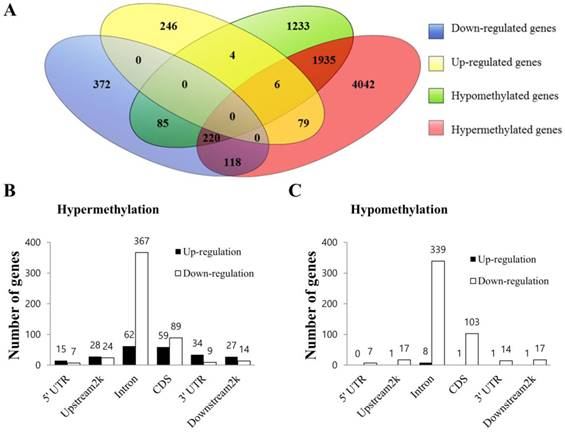
\includegraphics[width=0.8\textwidth]{journal-of-cancer_sample-result}}
% 	\caption{یک نمونه نمودار خلاصه برای نمایش نوآوری در نتایج
% 		%\cite{kim2016integrated}
% 	}
% 	\label{fig:sampleDiagram}
% \end{figure}\\
% طبیعتاً به صلاحدید نگارنده، شکل‌ها و نمودار‌ها می توانند در بخش های مختلف، خصوصا فصل
% \ref{chap:results}
% مورد استفاده قرار گیرند.

\subsection{تعریف واژه‌ها (اختیاری)}
% در این قسمت محقق باید واژه‌هایی را که ممکن است برای خواننده آشنا نباشد، تعریف کند.

\subsection{خلاصه فصل‌ها}
% در آخرین قسمتِ فصل اول پایان‌نامه، خلاصه‌ای اشاره‌وار از فصل‌های آتی آورده می‌شود تا خواننده بتواند تصویری واضح از دیگر قسمت‌های پایان‌نامه در ذهن خود ترسیم کند.

\section{جمع‌بندی}
% در این فصل به دو مقولهٔ نحوه استفاده از قالب \پ دانشگاه تهران و نیز ویژگی‌هایی که محتویات فصل اول پایان‌نامه (یعنی مقدمه) باید داشته باشند، پرداخته شد. با توجه به اینکه این راهنما نحوه استفاده از قالب را شرح داده، ملزومات محتوایی هر فصل پایان‌نامه را توضیح می‌دهد و در پیوست‌ها نیز نحوهٔ کار با لاتک را یادآوری خواهد کرد، بنابراین مطالعهٔ کامل آن مقداری وقت شما را خواهد گرفت؛ اما مطمئن باشید از اتلاف وقت شما در ادامه کارتان تا حد زیادی جلوگیری خواهد کرد. در نوشتن متن حاضر سعی شده است علاوه بر ایجاد یک قالب لاتک برای پایان‌نامه‌های دانشگاه تهران، نکات محتوایی هر فصل نیز گوشزد گردد. طبیعتاً برای نگارش پایان‌نامهٔ خود می‌بایست مطالب تمام فصل‌ها را خودتان بازنویسی کنید.

% در ادامهٔ این راهنما، تنها فصل‌هایی که یک پایان‌نامه باید داشته باشد و نیز خصوصیات یا ساختاری که محتویات هر فصل باید از آنها برخوردار باشد%
% \footnote{از روی فایل «تمپلیت نگارش و تدوین پایان‌نامه \cite{UTThesisGuide}»}،
% آورده می‌شوند. نهایتاً  در پیوست‌ها، مطالبی در باب یادآوری دستورات لاتک، نحوه نوشتن فرمول‌ها، تعاریف، قضایا، مثال‌ها، درج تصاویر، نمودارها، جداول و الگوریتم‌ها و نیز مدیریت مراجع، آمده است.

% همچنین توصیه اکید دارم که رفع خطاهایی که احتمالاً با آنها مواجه می‌شوید را به آخر موکول نفرمایید و به محض برخورد با خطا، آن را اشکال‌زدایی و برطرف نمائید.!
% و
% \verb!% !TeX root=main.tex
\chapter{مروری بر مطالعات انجام شده}
%\thispagestyle{empty} 
\section{مقدمه}
% هدف از اين فصل که با عنوان‌های  «مروری بر ادبیات موضوع%
% \LTRfootnote{Literature Review}»،
% «مروری بر منابع» و يا «مروری بر پیشینه تحقیق%
% \LTRfootnote{Background Research}»
% معرفی می‌شود، بررسی و طبقه‌بندی یافته‌های تحقیقات دیگر محققان در سطح دنیا و تعیین و شناسایی خلأهای تحقیقاتی است. آنچه را که تحقیق شما به دانش موجود اضافه می‌کند، مشخص کنید. طرح پیشینه تحقیق%
% \LTRfootnote{Background Information}
% یک مرور محققانه است و تا آنجا باید پیش برود که پیش‌زمینهٔ تاریخی مناسبی از تحقیق را بیان کند و جایگاه تحقیق فعلی را در میان آثار پیشین نشان دهد. برای این منظور منابع مرتبط با تحقیق را بررسی کنید، البته نه آنچنان گسترده که کل پیشینه تاریخی بحث را در برگیرد. برای نوشتن این بخش:
% \begin{itemize}
% 	\item
% 	دانستنی‌های موجود و پیش‌زمینهٔ تاریخی و وضعیت کنونی موضوع را چنان بیان کنید که خواننده بدون مراجعه به منابع پیشین، نتایج حاصل از مطالعات قبلی را درک و ارزیابی کند.
% 	\item
% 	نشان دهید که بر موضوع احاطه دارید. پرسش تحقیق را همراه بحث و جدل‌ها و مسائل مطرح شده بیان کنید و مهم‌ترین تحقیق‌های انجام شده در این زمینه را معرفی نمائید.
% 	\item
% 	ابتدا مطالب عمومی‌تر و سپس پژوهش‌های مشابه با کار خود را معرفی کرده و نشان دهید که تحقیق شما از چه جنبه‌ای با کار دیگران تشابه یا تفاوت دارد.
% 	\item
% 	اگر کارهای قبلی را خلاصه کرده‌اید، از پرداختن به جزئیات غیرضروری بپرهیزید. در عوض، بر یافته‌ها و مسائل روش‌شناختی مرتبط و نتایج اصلی تأکید کنید و اگر بررسی‌ها و منابع مروری عمومی دربارهٔ موضوع موجود است، خواننده را به آنها ارجاع دهید.
% \end{itemize}


% \section{مروری بر ادبیات موضوع}
% در این قسمت باید به کارهای مشابه دیگران در گذشته اشاره کرد و وزن بیشتر این قسمت بهتر است به مقالات ژورنالی سال‌های اخیر (۲ تا ۳ سال) تخصیص داده شود. به نتایج کارهای دیگران با ذکر دقیق مراجع باید اشاره شده و جایگاه و تفاوت تحقیق شما نیز با کارهای دیگران مشخص شود. استفاده از مقالات ژورنال‌های معتبر در دو یا سه سال اخیر، می‌تواند به اعتبار کار شما بیافزاید.

% \section{نتیجه‌گیری}
% ‌در نتیجه‌گیری آخر این فصل، با توجه به بررسی انجام شده بر روی مراجع تحقيق، بخش‌های قابل گسترش و تحقیق در آن حیطه و چشم‌اندازهای تحقیق مورد بررسی قرار می‌گیرند.	در برخی از تحقیقات، نتیجه نهایی فصل روش تحقیق، ارائهٔ یک چارچوب کار تحقیقی 
% \lr{(research framework)}
% است.
\ifExperimentalAuction
	تصمیم‌گیری های ما نمایشگر ارزشگذاری‌های ما هستند. اقتصاد‌دان‌ها
	\textit{ارزش اقتصادی}
	\LTRfootnote{economic value}
	این تصمیمات را با نرخی که فرد یک محصول یا دارایی را با  دیگری مبادله می کند ، بیان می‌کنند.
	این نرخ به وسیله
	\textit{تمایل به پرداخت }
	\LTRfootnote{willingness to pay}
	حداکثری فرد اندازه‌گیری می‌شود.
	\citep{luskExperimentalAuctionsMethods2007}
	\section{تعاریف، اصول و مبانی نظری}
	% این قسمت ارائهٔ خلاصه‌ای از دانش کلاسیک موضوع است. این بخش الزامی نیست و بستگی به نظر استاد راهنما دارد.

\fi

\ifTheEffectsOfDifferentPersonalData
	\textit{چاو، اوی و هربلاند}
	\LTRfootnote{Chua, H.N., J.S. Ooi, and A. Herbland}
	در سال ۲۰۲۱ اطلاعات شخصی را در ۶ دسته طبقه بندی کرده‌اند.
	\citep{chuaEffectsDifferentPersonal2021}
	جدول
	\eqref{tab:PICatAndChar}
	\begin{table}[ht]
		\caption{دسته‌ها و ویژگی‌های اطلاعت شخصی}
		\label{tab:PICatAndChar}
		\centering
		\onehalfspacing
		% \begin{tabular}{p{0.35\linewidth} | p{0.6\linewidth}}  
		\begin{tabularx}{\linewidth}{ r X }
			% \hline 
			دسته
			 &
			% درجه آزادی 
			% تبدیل مختصات &
			توضیح
			\\
			\hline
			سبک زندگی-رفتار(LB)
			 &
			% zotero://select/library/items/LCYS3GQ2
			% https://www.zotero.org/users/5038267/items/LCYS3GQ2
			%توضیح
			اطلاعت درباره ویژگی‌ها و سبک زندگی فرد که بر رابطه عاطفی یا
			اجتماعی، ترجیهات، عادات، باورها، یا دیدگاه‌های او اثر می‌گذارد.
			% مثال‌ها:
			% \lr{L1}:
			% باور
			% (
			% مانند باورهای مذهبی، باورهای فلسفی، افکار و غیره
			% )
			% % \hline 
			% \lr{L2}:
			% ترجیهات و علایق
			% (مانند نظرات، تمایلات، علایق، غذاهای مورد علاقه، رنگ‌ها، چیزهای
			% دوست‌داشتنی و دوست‌نداشتنی)
			% \lr{L3}:
			% رفتار
			% (مانند رفتار وبگردی، الگوی تماس‌ها، لینک‌های کلیک شده،
			% سبک زندگی رویکرد و غیره)
			% \lr{L4}:
			% خانواده/روابط عاطفی
			% (مانند ساختار خانواده، همشیرها، فرزندان، ازدواج‌ها، طلاق‌ها،
			% روابط عاطفی و غیره)
			\\
			اجتماعی-اقتصادی(SE)
			 &
			% ۳ & 
			% ویژگی دو &
			اطلاعاتی که سطح زندگی اقتصادی یا اجتماعی فرد را نشان می‌دهند یا
			می‌توان به وسیله این اطلاعات ویژگی‌های مزبور را استخراج کرد.
			% مثال‌ها;
			% \lr{S1}:
			% \lr{S1}:
			% \lr{S1}:
			\\
			ردیابی(T)
			 &
			اطلاعاتی که روش‌هایی را برای موقعیت‌یابی و تماس با فرد ایجاد می کند.
			% \hline 
			\\
			اقتصادی(F)
			 &
			اطلاعاتی که درآمد، حساب‌های مالی، اعتبار، توانایی خرید/خرج کردن، و
			دارایی‌های مورد تملک/اجاره شده/قرض گرفته شده را مشخص می کند.
			\\
			احراز هویت(A)
			 &
			اطلاعاتی که برای احراز هویت فرد به کار می‌روند.
			\\
			پزشکی-سلامت(MH)
			 &
			شرایط پزشکی  یا اطلاعات مرتبط با سلامت فرد.
			\\
		\end{tabularx}
	\end{table}
	% \begin{table}[ht]
	%     \caption{مدلهای تبدیل دیگر.}
	%     \label{tab:motionModelsCont}
	%     \centering
	%     \onehalfspacing
	%     \begin{tabularx}{\textwidth}{|r|c|l|X|}
	%         \hline نام مدل & درجه آزادی & تبدیل مختصات & توضیح \\ 
	%         \hline مشابهت & ۴ & $\begin{aligned} x'=sx\cos\theta - sy\sin\theta+t_x \\ y'=sx\sin\theta+sy\cos\theta+t_y  \end{aligned}$  & اقلیدسی+تغییرمقیاس \\ 		
	%         \hline آفین & ۶ & $\begin{aligned} x'=a_{11}x+a_{12}y+t_x \\ y'=a_{21}x+a_{22}y+t_y \end{aligned}$  & مشابهت+اریب‌شدگی \\
	%         \hline
	%     \end{tabularx}
	% \end{table}


	از سوی دیگر
\fi %TheEffectsOfDifferentPersonalData
\ifMultidimensionalNatureOfPrivacyRisksConceptualisationMeasurementAndImplicationsForDigitalServices
	در سال ۲۰۲۲
	\textit{
		\gls{Sabrina Karwatzki, Manuel Trenz and Daniel Veit}
	}
	 یک دسته‌بندی قاعده‌گرا
	\textit{
		\gls{Nomological}
	}
	و جامع از نگرانی‌های حریم خصوصی افراد بر اساس پژوهش های گذشته ارائه داده و اعتبار و روایی آن‌را مورد سنجش قرار‌داده‌اند
	\citep{karwatzkiMultidimensionalNaturePrivacy}
	\!.
	آنها ۷ دسته
	\textbf{
		خطر حریم خصوصی فیزیکی
		\lr{(PH)}
		\LTRfootnote{Physical privacy risk}
		،
		خطر حریم خصوصی اجتماعی
		\lr{(SO)}
		\LTRfootnote{Social privacy risk}
		،
		خطر حریم خصوصی مرتبط با منابع
		\lr{(RE)}
		\LTRfootnote{Resource-related privacy risk}
		،
		خطر حریم خصوصی روانشناختی
		\lr{(PS)}
		\LTRfootnote{Psychological privacy risk}
		،
		خطر حریم خصوصی مرتبط با تعقیب قانونی
		\lr{(PR)}
		\LTRfootnote{Prosecution-related privacy risk}
		،
		خطر حریم خصوصی مرتبط با شغل
		\lr{(CR)}
		\LTRfootnote{Career-related privacy risks}
		\textmd{و}
		خطر حریم خصوصی مرتبط با آزادی
		\lr{(FR)}
		\LTRfootnote{Freedom-related privacy risk}
	}
\fi %\ifMultidimensionalNatureOfPrivacyRisksConceptualisationMeasurementAndImplicationsForDigitalServices
را شناسایی کردند. ما
از این دسته‌بندی و توصیفاتی که در این پژوهش با دسته‌بندی‌های نامبرده مرتبط دانسته شده اند، استفاده کردیم.
!
% را در فایل 
% \lr{main.tex}،
% غیرفعال%
% \footnote{
% برای غیرفعال کردن یک دستور، کافی است در ابتدای آن، علامت درصد انگلیسی (\%) بگذارید.
% }
%  کنید. در غیر این صورت، ابتدا مطالب دو فصل اول پردازش شده و سپس مطالب فصل ۳ پردازش می‌شود که این کار باعث طولانی شدن زمان پردازش می‌گردد. هر زمان که خروجی کل \پ را خواستید، تمام فصل‌ها را دوباره در
% \lr{main.tex}
% فعال نمائید.
% بدیهتاً لازم نیست فصل‌های \پ را به ترتیب تایپ کنید. مثلاً می‌توانید ابتدا مطالب فصل ۳ را تایپ نموده و سپس مطالب فصل ۱ را تایپ کنید. 
% \subsubsection{مراجع}
% برای وارد کردن مراجع \پ کافی است فایل 
% \lr{MyReferences.bib}
% را باز کرده و مراجع خود را به شکل اقلام نمونهٔ داخل آن، وارد کنید.  سپس از \lr{bibtex} برای تولید مراجع با قالب مناسب استفاده نمائید. برای توضیحات بیشتر بخش \ref{Sec:Ref} از پیوست \ref{app:latexIntro} و نیز پیوست \ref{app:refMan} را ببینید.

% \subsubsection{واژه‌نامه فارسی به انگلیسی و برعکس}
% برای وارد کردن معادل فارسی اصطلاحات لاتین در متن و تهیه فهرست واژه‌نامه از آنها، از بستهٔ
% \lr{glossaries}
% و نرم‌افزار
% \lr{xindy}
% استفاده می‌شود. بدین منظور کافی است اصطلاحات لاتین و ترجمهٔ آنها را در فایل
% \lr{words.tex}
% وارد کرده و هر جای متن که خواستید با دستورات
% \verb|gls{label}|
% یا \verb|glspl{label}|
% معادل فارسی مفرد یا جمع یک اصطلاح را بیاورید.

% مثلا در اینجا، واژهٔ
% «\gls{Action}»
% برای بار اول و دوباره
% «\gls{Action}»
% برای بار دوم در متن ظاهر شده است.
% جهت توضیحات بیشتر به پیوست
% \ref{app:refMan}
% مراجعه کنید.
% \subsubsection{نمایه}
% برای وارد کردن نمایه، باید از 
% \lr{xindy}
% استفاده کنید. 
%زیرا 
%\lr{MakeIndex}
%با حروف «گ»، «چ»، «پ»، «ژ» و «ک» مشکل دارد و ترتیب الفبایی این حروف را رعایت نمی‌کند. همچنین، فاصله بین هر گروه از کلمات در 
%\lr{MakeIndex}،
%به درستی رعایت نمی‌شود که باعث زشت شدن حروف‌چینی این قسمت می‌شود. 
% راهنمای چگونگی کار با 
% \lr{xindy} 
% را می‌توانید در ویکی پارسی‌لاتک و یا مثالهای موجود در دی‌وی‌دی «مجموعه پارسی‌لاتک»، پیدا کنید.

% \subsection{اگر سوالی داشتم، از کی بپرسم؟}
% برای پرسیدن سوال‌های خود موقع حروف‌چینی با زی‌پرشین، می‌توانید به
% \href{http://qa.parsilatex.com}{سایت پرسش و پاسخ پارسی‌لاتک}%
% \LTRfootnote{http://qa.parsilatex.com}
% یا
% \href{http://forum.parsilatex.com}{بایگانی تالارگفتگوی قدیمی پارسی‌لاتک}%
% \mypagestye{http://forum.parsilatex.com}
% مراجعه کنید. شما هم می‌توانید روزی به سوال‌های دیگران در اینترنت جواب دهید.
% بستهٔ زی‌پرشین و بسیاری از بسته‌های مرتبط با آن مانند
% \lr{bidi} و
% \lr{Persian-bib}،
% مجموعه پارسی‌لاتک، مثالهای مختلف موجود در آن، قالب پایان‌نامه دانشگاههای مختلف و سایت پارسی‌لاتک همه به صورت داوطلبانه توسط افراد گروه پارسی‌لاتک و گروه
% \lr{Persian TeX}
% و بدون هیچ کمک مالی انجام شده‌اند. کار اصلی نوشتن و توسعه زی‌پرشین توسط آقای وفا خلیقی انجام شده است که این کار بزرگ را به انجام رساندند.
% اگر مایل به کمک به گروه پارسی‌لاتک هستید به سایت این گروه مراجعه فرمایید:
% \begin{center}
% 	\url{http://www.parsilatex.com}
% \end{center}

% \section{محتویات فصل اول یک پایان‌نامه}
% فصل اول یک پایان‌نامه باید به مقدمه یا کلیات تحقیق بپردازد.
% هدف از فصل مقدمه%
% \LTRfootnote{Introduction}،
% شرح مختصر مسأله تحقیق، اهمیت و انگیزه محقق از پرداختن به آن موضوع، بهمراه اشاره‌ای كوتاه به روش و مراحل تحقیق است. مقدمه، اولين فصل از ساختار اصلی \پ بوده و زمینه اطلاعاتی لازم را برای خواننده فراهم می‌آورد. در طول مقدمه باید سعی شود موضوع تحقیق با زبانی روشن، ساده و بطور عمیق و هدفمند به خواننده معرفی شود. این فصل باید خواننده را مجذوب و اهميت موضوع تحقيق را آشکار سازد. در مقدمه باید با ارائهٔ سوابق، شواهد تحقيقی و اطلاعات موجود (با ذکر منبع) با روشی منظم، منطقی و هدف‌دار، خواننده را جهت داد و به سوی راه حل مورد نظر هدايت کرد. مقدمه مناسب‌ترين جا برای ارائهٔ اختصارات و بعضی توضيحات کلی است، توضيحاتی که شايد نتوان در مباحث ديگر آنها را شرح داد.

% مقدمه، یکی از ارکان اساسی و اصلی پایان نامه است که مهمترین قسمت‌های آن عبارتند از: 

% \subsection{عنوان تحقیق} 
% باید شناختی دقیق و روشن از حوزهٔ موضوع تحقیق را عرضه دارد و خالی از هرگونه ابهام و پیچیدگی باشد.

% \subsection{مسأله تحقیق}
% وظیفه اصلی مقدمه بیان این مطلب به خواننده است که چرا انجام تحقیق را به عهده گرفته‌اید. اگر دلیل شما برای انجام این کار پاسخگویی به سؤال مورد علاقه‌تان است، با مشکل زیادی روبه‌رو نخواهید بود. یکی از بهترین روش‌ها برای نوشتن مقدمهٔ یک پایان‌نامه، طرح پرسش یا پرسش‌هایی مهم و اساسی است که کار تحقیقاتی شما از آغاز تا پایان قصد پاسخ دادن به آن را دارد. گاهی می‌توانید ابتدا اهمیت موضوع را بیان و سپس پرسش خود را در آن موضوع مطرح کنید.

% \subsection{تاریخچه‌ای از موضوع تحقیق}
% به طور کلی تشریح روندهای تحقیقاتی در محدودهٔ مورد مطالعه، مستلزم ارجاع به کارهای دیگران است. بعضی از نویسندگان برای کارهای دیگران هیچ اعتباری قائل نمی‌شوند و در مقابل، بعضی دیگر از نویسندگان در توصیف کارهای دیگران، بسیار زیاده‌روی می‌کنند. اکثر مواقع، ارجاع به مقالات دو سال قبل از کارتان، بهتر از نوشتن سطرهای مرجع است. در این قسمت باید به طور مختصر به نظرات و تحقیقات مربوط به موضوع و یا مسائل و مشکلات حل نشده در این حوزه و همچنین توجه و علاقه جامعه به این موضوع، اشاره شود.

% \subsection{تعریف موضوع تحقیق}
% در این قسمت محقق، موضوع مورد علاقه و یا نیاز احساس شدهٔ خود را در حوزه تحقیق بیان می‌دارد و عوامل موجود در موقعیت را تعریف و تعیین می‌کند.

% \subsection{هدف یا هدف‌های کلی و آرمانی تحقیق}
% این قسمت باید با جملات مثبت و کلی طرح شود و از طولانی شدن مطالب پرهیز شود.

% \subsection{روش انجام تحقیق}
% در این قسمت، پژوهشگر روش کاری خود را بیان می‌دارد و شیوه‌های گوناگونی را که در گردآوری مطالب خود بکار برده، ذکر می‌کند. همچنین اگر روش آماری خاصی را در تهیه و تدوین اطلاعات به کار برده است، آن شیوه را نیز اینجا بیان می‌کند.

% \subsection{نوآوری، اهمیت و ارزش تحقیق}
% در این قسمت، در مورد نوآوری علمی و عملی تحقیق که محقق به آن دست خواهد یافت، بحث می‌شود. ممکن است لازم باشد تا برخی نمودارهای خلاصه در این بخش استفاده شوند. به عنوان مثال، نموداری از مقاله
% \citep{kim2016integrated}
% در شکل
% \ref{fig:sampleDiagram}
% آمده است.
% \begin{figure}[ht]
% 	\centerline{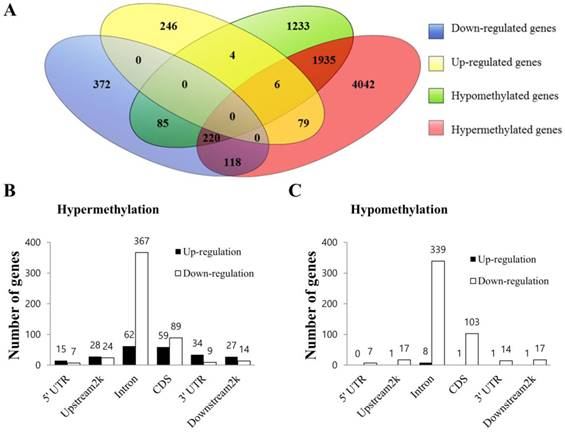
\includegraphics[width=0.8\textwidth]{journal-of-cancer_sample-result}}
% 	\caption{یک نمونه نمودار خلاصه برای نمایش نوآوری در نتایج
% 		%\citep{kim2016integrated}
% 	}
% 	\label{fig:sampleDiagram}
% \end{figure}\\
% طبیعتاً به صلاحدید نگارنده، شکل‌ها و نمودار‌ها می توانند در بخش های مختلف، خصوصا فصل
% \ref{chap:results}
% مورد استفاده قرار گیرند.

% \subsection{تعریف واژه‌ها (اختیاری)}
% در این قسمت محقق باید واژه‌هایی را که ممکن است برای خواننده آشنا نباشد، تعریف کند.

% \subsection{خلاصه فصل‌ها}
% در آخرین قسمتِ فصل اول پایان‌نامه، خلاصه‌ای اشاره‌وار از فصل‌های آتی آورده می‌شود تا خواننده بتواند تصویری واضح از دیگر قسمت‌های پایان‌نامه در ذهن خود ترسیم کند.
در ادامه این پایان‌نامه، در بخش دوم گزارشی از پژوهش‌های پیشین مربتط با موضوع این پایان‌نامه ارائه می‌شود.
در بخش سوم روش انجام تحقیق انجام شده توضیح داده می شود
\!.
تعریف عملیاتی و نظری متغیر‌های اندازه‌گیری شده در این آزمایش، روش نمونه‌گیری و معرفی ابزارها و پرسشنامه‌ها در این بخش قرار دارند
\!.
سپس در بخش چهارم نتایج کمی به دست آمده پس از انجام آزمایش از اطلاعات جمع آوری شده، ارائه می‌شوند
\!.
در این بخش  روش به کار رفته برای تحلیل داده‌ها و آزمون فرضیه‌های پژوهشی و نتایج  به دست آمده، درج  می‌شوند
\!.
نمودار‌هایی تولید شده برای نمایش کیفی نتایج نیز در بخش چهارم هستند.
در بخش پنجم با در نظر گرفتن پژوهش‌های انجام شده و نظریه‌های موجود و شرایط و محدودیت‌ای این پژوهش و ویژگی‌های نمونه، نتایج گزارش شده در بخش چهارم مورد بحث و بررسی
قرار می‌گیرند و پیشهادهایی برای پژوهش‌های آینده ارائه می‌شوند.
% \section{جمع‌بندی}

در بخش ابتدایی این پایان‌نامه تلاش کردیم تا روند شکل گیری سوال پژوهشی و اهمیت آن را توضیح دهیم.
همچنین نظریه‌هایی که برای توصیف رفتار افراد وجود دارند را معرفی کردیم و از آن‌ها به عنوان راهنمایی
برای ارائه فرضیه‌های پژوهشی مرتبط با سوال‌ مطرح شده، استفاده کردیم.
همچنین، پژوهش‌های انجام شده که مبنای نظریه‌های توصیف کننده رفتار به اشتراک گذاری اطلاعات خصوصی دیگران
بوده‌اند، به اختصار معرفی شدند. در بخش بعد، به مرور پژوهش‌هایی می‌پردازیم که با سوال پژوهشی و فرضیه‌های این پایان‌نامه مرتبط هستند.

% در این فصل به دو مقولهٔ نحوه استفاده از قالب \پ دانشگاه تهران و نیز ویژگی‌هایی که محتویات فصل اول پایان‌نامه (یعنی مقدمه) باید داشته باشند، پرداخته شد. با توجه به اینکه این راهنما نحوه استفاده از قالب را شرح داده، ملزومات محتوایی هر فصل پایان‌نامه را توضیح می‌دهد و در پیوست‌ها نیز نحوهٔ کار با لاتک را یادآوری خواهد کرد، بنابراین مطالعهٔ کامل آن مقداری وقت شما را خواهد گرفت؛ اما مطمئن باشید از اتلاف وقت شما در ادامه کارتان تا حد زیادی جلوگیری خواهد کرد. در نوشتن متن حاضر سعی شده است علاوه بر ایجاد یک قالب لاتک برای پایان‌نامه‌های دانشگاه تهران، نکات محتوایی هر فصل نیز گوشزد گردد. طبیعتاً برای نگارش پایان‌نامهٔ خود می‌بایست مطالب تمام فصل‌ها را خودتان بازنویسی کنید.

% در ادامهٔ این راهنما، تنها فصل‌هایی که یک پایان‌نامه باید داشته باشد و نیز خصوصیات یا ساختاری که محتویات هر فصل باید از آنها برخوردار باشد%
% \footnote{از روی فایل «تمپلیت نگارش و تدوین پایان‌نامه \citep{UTThesisGuide}»}،
% آورده می‌شوند. نهایتاً  در پیوست‌ها، مطالبی در باب یادآوری دستورات لاتک، نحوه نوشتن فرمول‌ها، تعاریف، قضایا، مثال‌ها، درج تصاویر، نمودارها، جداول و الگوریتم‌ها و نیز مدیریت مراجع، آمده است.

% همچنین توصیه اکید دارم که رفع خطاهایی که احتمالاً با آنها مواجه می‌شوید را به آخر موکول نفرمایید و به محض برخورد با خطا، آن را اشکال‌زدایی و برطرف نمائید.